%********************************************%
%*       Generated from PreTeXt source      *%
%*       on 2020-12-29T14:25:13-03:00       *%
%*   A recent stable commit (2020-08-09):   *%
%* 98f21740783f166a773df4dc83cab5293ab63a4a *%
%*                                          *%
%*         https://pretextbook.org          *%
%*                                          *%
%********************************************%
\documentclass[oneside,10pt,]{book}
%% Custom Preamble Entries, early (use latex.preamble.early)
%% Default LaTeX packages
%%   1.  always employed (or nearly so) for some purpose, or
%%   2.  a stylewriter may assume their presence
\usepackage{geometry}
%% Some aspects of the preamble are conditional,
%% the LaTeX engine is one such determinant
\usepackage{ifthen}
%% etoolbox has a variety of modern conveniences
\usepackage{etoolbox}
\usepackage{ifxetex,ifluatex}
%% Raster graphics inclusion
\usepackage{graphicx}
%% Color support, xcolor package
%% Always loaded, for: add/delete text, author tools
%% Here, since tcolorbox loads tikz, and tikz loads xcolor
\PassOptionsToPackage{usenames,dvipsnames,svgnames,table}{xcolor}
\usepackage{xcolor}
%% begin: defined colors, via xcolor package, for styling
%% end: defined colors, via xcolor package, for styling
%% Colored boxes, and much more, though mostly styling
%% skins library provides "enhanced" skin, employing tikzpicture
%% boxes may be configured as "breakable" or "unbreakable"
%% "raster" controls grids of boxes, aka side-by-side
\usepackage{tcolorbox}
\tcbuselibrary{skins}
\tcbuselibrary{breakable}
\tcbuselibrary{raster}
%% We load some "stock" tcolorbox styles that we use a lot
%% Placement here is provisional, there will be some color work also
%% First, black on white, no border, transparent, but no assumption about titles
\tcbset{ bwminimalstyle/.style={size=minimal, boxrule=-0.3pt, frame empty,
colback=white, colbacktitle=white, coltitle=black, opacityfill=0.0} }
%% Second, bold title, run-in to text/paragraph/heading
%% Space afterwards will be controlled by environment,
%% independent of constructions of the tcb title
%% Places \blocktitlefont onto many block titles
\tcbset{ runintitlestyle/.style={fonttitle=\blocktitlefont\upshape\bfseries, attach title to upper} }
%% Spacing prior to each exercise, anywhere
\tcbset{ exercisespacingstyle/.style={before skip={1.5ex plus 0.5ex}} }
%% Spacing prior to each block
\tcbset{ blockspacingstyle/.style={before skip={2.0ex plus 0.5ex}} }
%% xparse allows the construction of more robust commands,
%% this is a necessity for isolating styling and behavior
%% The tcolorbox library of the same name loads the base library
\tcbuselibrary{xparse}
%% Hyperref should be here, but likes to be loaded late
%%
%% Inline math delimiters, \(, \), need to be robust
%% 2016-01-31:  latexrelease.sty  supersedes  fixltx2e.sty
%% If  latexrelease.sty  exists, bugfix is in kernel
%% If not, bugfix is in  fixltx2e.sty
%% See:  https://tug.org/TUGboat/tb36-3/tb114ltnews22.pdf
%% and read "Fewer fragile commands" in distribution's  latexchanges.pdf
\IfFileExists{latexrelease.sty}{}{\usepackage{fixltx2e}}
%% Text height identically 9 inches, text width varies on point size
%% See Bringhurst 2.1.1 on measure for recommendations
%% 75 characters per line (count spaces, punctuation) is target
%% which is the upper limit of Bringhurst's recommendations
\geometry{letterpaper,total={340pt,9.0in}}
%% Custom Page Layout Adjustments (use latex.geometry)
%% This LaTeX file may be compiled with pdflatex, xelatex, or lualatex executables
%% LuaTeX is not explicitly supported, but we do accept additions from knowledgeable users
%% The conditional below provides  pdflatex  specific configuration last
%% begin: engine-specific capabilities
\ifthenelse{\boolean{xetex} \or \boolean{luatex}}{%
%% begin: xelatex and lualatex-specific default configuration
\ifxetex\usepackage{xltxtra}\fi
%% realscripts is the only part of xltxtra relevant to lualatex 
\ifluatex\usepackage{realscripts}\fi
%% end:   xelatex and lualatex-specific default configuration
}{
%% begin: pdflatex-specific default configuration
%% We assume a PreTeXt XML source file may have Unicode characters
%% and so we ask LaTeX to parse a UTF-8 encoded file
%% This may work well for accented characters in Western language,
%% but not with Greek, Asian languages, etc.
%% When this is not good enough, switch to the  xelatex  engine
%% where Unicode is better supported (encouraged, even)
\usepackage[utf8]{inputenc}
%% end: pdflatex-specific default configuration
}
%% end:   engine-specific capabilities
%%
%% Fonts.  Conditional on LaTex engine employed.
%% Default Text Font: The Latin Modern fonts are
%% "enhanced versions of the [original TeX] Computer Modern fonts."
%% We use them as the default text font for PreTeXt output.
%% Default Monospace font: Inconsolata (aka zi4)
%% Sponsored by TUG: http://levien.com/type/myfonts/inconsolata.html
%% Loaded for documents with intentional objects requiring monospace
%% See package documentation for excellent instructions
%% fontspec will work universally if we use filename to locate OTF files
%% Loads the "upquote" package as needed, so we don't have to
%% Upright quotes might come from the  textcomp  package, which we also use
%% We employ the shapely \ell to match Google Font version
%% pdflatex: "varl" package option produces shapely \ell
%% pdflatex: "var0" package option produces plain zero (not used)
%% pdflatex: "varqu" package option produces best upright quotes
%% xelatex,lualatex: add OTF StylisticSet 1 for shapely \ell
%% xelatex,lualatex: add OTF StylisticSet 2 for plain zero (not used)
%% xelatex,lualatex: add OTF StylisticSet 3 for upright quotes
%%
%% Automatic Font Control
%% Portions of a document, are, or may, be affected by defined commands
%% These are perhaps more flexible when using  xelatex  rather than  pdflatex
%% The following definitions are meant to be re-defined in a style, using \renewcommand
%% They are scoped when employed (in a TeX group), and so should not be defined with an argument
\newcommand{\divisionfont}{\relax}
\newcommand{\blocktitlefont}{\relax}
\newcommand{\contentsfont}{\relax}
\newcommand{\pagefont}{\relax}
\newcommand{\tabularfont}{\relax}
\newcommand{\xreffont}{\relax}
\newcommand{\titlepagefont}{\relax}
%%
\ifthenelse{\boolean{xetex} \or \boolean{luatex}}{%
%% begin: font setup and configuration for use with xelatex
%% Generally, xelatex is necessary for non-Western fonts
%% fontspec package provides extensive control of system fonts,
%% meaning *.otf (OpenType), and apparently *.ttf (TrueType)
%% that live *outside* your TeX/MF tree, and are controlled by your *system*
%% (it is possible that a TeX distribution will place fonts in a system location)
%%
%% The fontspec package is the best vehicle for using different fonts in  xelatex
%% So we load it always, no matter what a publisher or style might want
%%
\usepackage{fontspec}
%%
%% begin: xelatex main font ("font-xelatex-main" template)
%% Latin Modern Roman is the default font for xelatex and so is loaded with a TU encoding
%% *in the format* so we can't touch it, only perhaps adjust it later
%% in one of two ways (then known by NFSS names such as "lmr")
%% (1) via NFSS with font family names such as "lmr" and "lmss"
%% (2) via fontspec with commands like \setmainfont{Latin Modern Roman}
%% The latter requires the font to be known at the system-level by its font name,
%% but will give access to OTF font features through optional arguments
%% https://tex.stackexchange.com/questions/470008/
%% where-and-how-does-fontspec-sty-specify-the-default-font-latin-modern-roman
%% http://tex.stackexchange.com/questions/115321
%% /how-to-optimize-latin-modern-font-with-xelatex
%%
%% end:   xelatex main font ("font-xelatex-main" template)
%% begin: xelatex mono font ("font-xelatex-mono" template)
%% (conditional on non-trivial uses being present in source)
\IfFontExistsTF{Inconsolatazi4-Regular.otf}{}{\GenericError{}{The font "Inconsolatazi4-Regular.otf" requested by PreTeXt output is not available.  Either a file cannot be located in default locations via a filename, or a font is not known by its name as part of your system.}{Consult the PreTeXt Guide for help with LaTeX fonts.}{}}
\IfFontExistsTF{Inconsolatazi4-Bold.otf}{}{\GenericError{}{The font "Inconsolatazi4-Bold.otf" requested by PreTeXt output is not available.  Either a file cannot be located in default locations via a filename, or a font is not known by its name as part of your system.}{Consult the PreTeXt Guide for help with LaTeX fonts.}{}}
\usepackage{zi4}
\setmonofont[BoldFont=Inconsolatazi4-Bold.otf,StylisticSet={1,3}]{Inconsolatazi4-Regular.otf}
%% end:   xelatex mono font ("font-xelatex-mono" template)
%% begin: xelatex font adjustments ("font-xelatex-style" template)
%% end:   xelatex font adjustments ("font-xelatex-style" template)
%%
%% Extensive support for other languages
\usepackage{polyglossia}
%% Set main/default language based on pretext/@xml:lang value
%% Enable secondary languages based on discovery of @xml:lang values
%% Enable fonts/scripts based on discovery of @xml:lang values
%% Western languages should be ably covered by Latin Modern Roman
%% end:   font setup and configuration for use with xelatex
}{%
%% begin: font setup and configuration for use with pdflatex
%% begin: pdflatex main font ("font-pdflatex-main" template)
\usepackage{lmodern}
\usepackage[T1]{fontenc}
%% end:   pdflatex main font ("font-pdflatex-main" template)
%% begin: pdflatex mono font ("font-pdflatex-mono" template)
%% (conditional on non-trivial uses being present in source)
\usepackage[varqu,varl]{inconsolata}
%% end:   pdflatex mono font ("font-pdflatex-mono" template)
%% begin: pdflatex font adjustments ("font-pdflatex-style" template)
%% end:   pdflatex font adjustments ("font-pdflatex-style" template)
%% end:   font setup and configuration for use with pdflatex
}
%% Symbols, align environment, commutative diagrams, bracket-matrix
\usepackage{amsmath}
\usepackage{amscd}
\usepackage{amssymb}
%% allow page breaks within display mathematics anywhere
%% level 4 is maximally permissive
%% this is exactly the opposite of AMSmath package philosophy
%% there are per-display, and per-equation options to control this
%% split, aligned, gathered, and alignedat are not affected
\allowdisplaybreaks[4]
%% allow more columns to a matrix
%% can make this even bigger by overriding with  latex.preamble.late  processing option
\setcounter{MaxMatrixCols}{30}
%%
%%
%% Division Titles, and Page Headers/Footers
%% titlesec package, loading "titleps" package cooperatively
%% See code comments about the necessity and purpose of "explicit" option.
%% The "newparttoc" option causes a consistent entry for parts in the ToC 
%% file, but it is only effective if there is a \titleformat for \part.
%% "pagestyles" loads the  titleps  package cooperatively.
\usepackage[explicit, newparttoc, pagestyles]{titlesec}
%% The companion titletoc package for the ToC.
\usepackage{titletoc}
%% Fixes a bug with transition from chapters to appendices in a "book"
%% See generating XSL code for more details about necessity
\newtitlemark{\chaptertitlename}
%% begin: customizations of page styles via the modal "titleps-style" template
%% Designed to use commands from the LaTeX "titleps" package
%% Plain pages should have the same font for page numbers
\renewpagestyle{plain}{%
\setfoot{}{\pagefont\thepage}{}%
}%
%% Single pages as in default LaTeX
\renewpagestyle{headings}{%
\sethead{\pagefont\slshape\MakeUppercase{\ifthechapter{\chaptertitlename\space\thechapter.\space}{}\chaptertitle}}{}{\pagefont\thepage}%
}%
\pagestyle{headings}
%% end: customizations of page styles via the modal "titleps-style" template
%%
%% Create globally-available macros to be provided for style writers
%% These are redefined for each occurence of each division
\newcommand{\divisionnameptx}{\relax}%
\newcommand{\titleptx}{\relax}%
\newcommand{\subtitleptx}{\relax}%
\newcommand{\shortitleptx}{\relax}%
\newcommand{\authorsptx}{\relax}%
\newcommand{\epigraphptx}{\relax}%
%% Create environments for possible occurences of each division
%% Environment for a PTX "preface" at the level of a LaTeX "chapter"
\NewDocumentEnvironment{preface}{mmmmmm}
{%
\renewcommand{\divisionnameptx}{Prefácio}%
\renewcommand{\titleptx}{#1}%
\renewcommand{\subtitleptx}{#2}%
\renewcommand{\shortitleptx}{#3}%
\renewcommand{\authorsptx}{#4}%
\renewcommand{\epigraphptx}{#5}%
\chapter*{#1}%
\addcontentsline{toc}{chapter}{#3}
\label{#6}%
}{}%
%% Environment for a PTX "chapter" at the level of a LaTeX "chapter"
\NewDocumentEnvironment{chapterptx}{mmmmmm}
{%
\renewcommand{\divisionnameptx}{Capítulo}%
\renewcommand{\titleptx}{#1}%
\renewcommand{\subtitleptx}{#2}%
\renewcommand{\shortitleptx}{#3}%
\renewcommand{\authorsptx}{#4}%
\renewcommand{\epigraphptx}{#5}%
\chapter[{#3}]{#1}%
\label{#6}%
}{}%
%% Environment for a PTX "section" at the level of a LaTeX "section"
\NewDocumentEnvironment{sectionptx}{mmmmmm}
{%
\renewcommand{\divisionnameptx}{Seção}%
\renewcommand{\titleptx}{#1}%
\renewcommand{\subtitleptx}{#2}%
\renewcommand{\shortitleptx}{#3}%
\renewcommand{\authorsptx}{#4}%
\renewcommand{\epigraphptx}{#5}%
\section[{#3}]{#1}%
\label{#6}%
}{}%
%% Environment for a PTX "subsection" at the level of a LaTeX "subsection"
\NewDocumentEnvironment{subsectionptx}{mmmmmm}
{%
\renewcommand{\divisionnameptx}{Subseção}%
\renewcommand{\titleptx}{#1}%
\renewcommand{\subtitleptx}{#2}%
\renewcommand{\shortitleptx}{#3}%
\renewcommand{\authorsptx}{#4}%
\renewcommand{\epigraphptx}{#5}%
\subsection[{#3}]{#1}%
\label{#6}%
}{}%
%% Environment for a PTX "exercises" at the level of a LaTeX "subsection"
\NewDocumentEnvironment{exercises-subsection}{mmmmmm}
{%
\renewcommand{\divisionnameptx}{Exercícios}%
\renewcommand{\titleptx}{#1}%
\renewcommand{\subtitleptx}{#2}%
\renewcommand{\shortitleptx}{#3}%
\renewcommand{\authorsptx}{#4}%
\renewcommand{\epigraphptx}{#5}%
\subsection[{#3}]{#1}%
\label{#6}%
}{}%
%% Environment for a PTX "exercises" at the level of a LaTeX "subsection"
\NewDocumentEnvironment{exercises-subsection-numberless}{mmmmmm}
{%
\renewcommand{\divisionnameptx}{Exercícios}%
\renewcommand{\titleptx}{#1}%
\renewcommand{\subtitleptx}{#2}%
\renewcommand{\shortitleptx}{#3}%
\renewcommand{\authorsptx}{#4}%
\renewcommand{\epigraphptx}{#5}%
\subsection*{#1}%
\addcontentsline{toc}{subsection}{#3}
\label{#6}%
}{}%
%%
%% Styles for six traditional LaTeX divisions
\titleformat{\part}[display]
{\divisionfont\Huge\bfseries\centering}{\divisionnameptx\space\thepart}{30pt}{\Huge#1}
[{\Large\centering\authorsptx}]
\titleformat{\chapter}[display]
{\divisionfont\huge\bfseries}{\divisionnameptx\space\thechapter}{20pt}{\Huge#1}
[{\Large\authorsptx}]
\titleformat{name=\chapter,numberless}[display]
{\divisionfont\huge\bfseries}{}{0pt}{#1}
[{\Large\authorsptx}]
\titlespacing*{\chapter}{0pt}{50pt}{40pt}
\titleformat{\section}[hang]
{\divisionfont\Large\bfseries}{\thesection}{1ex}{#1}
[{\large\authorsptx}]
\titleformat{name=\section,numberless}[block]
{\divisionfont\Large\bfseries}{}{0pt}{#1}
[{\large\authorsptx}]
\titlespacing*{\section}{0pt}{3.5ex plus 1ex minus .2ex}{2.3ex plus .2ex}
\titleformat{\subsection}[hang]
{\divisionfont\large\bfseries}{\thesubsection}{1ex}{#1}
[{\normalsize\authorsptx}]
\titleformat{name=\subsection,numberless}[block]
{\divisionfont\large\bfseries}{}{0pt}{#1}
[{\normalsize\authorsptx}]
\titlespacing*{\subsection}{0pt}{3.25ex plus 1ex minus .2ex}{1.5ex plus .2ex}
\titleformat{\subsubsection}[hang]
{\divisionfont\normalsize\bfseries}{\thesubsubsection}{1em}{#1}
[{\small\authorsptx}]
\titleformat{name=\subsubsection,numberless}[block]
{\divisionfont\normalsize\bfseries}{}{0pt}{#1}
[{\normalsize\authorsptx}]
\titlespacing*{\subsubsection}{0pt}{3.25ex plus 1ex minus .2ex}{1.5ex plus .2ex}
\titleformat{\paragraph}[hang]
{\divisionfont\normalsize\bfseries}{\theparagraph}{1em}{#1}
[{\small\authorsptx}]
\titleformat{name=\paragraph,numberless}[block]
{\divisionfont\normalsize\bfseries}{}{0pt}{#1}
[{\normalsize\authorsptx}]
\titlespacing*{\paragraph}{0pt}{3.25ex plus 1ex minus .2ex}{1.5em}
%%
%% Styles for five traditional LaTeX divisions
\titlecontents{part}%
[0pt]{\contentsmargin{0em}\addvspace{1pc}\contentsfont\bfseries}%
{\Large\thecontentslabel\enspace}{\Large}%
{}%
[\addvspace{.5pc}]%
\titlecontents{chapter}%
[0pt]{\contentsmargin{0em}\addvspace{1pc}\contentsfont\bfseries}%
{\large\thecontentslabel\enspace}{\large}%
{\hfill\bfseries\thecontentspage}%
[\addvspace{.5pc}]%
\dottedcontents{section}[3.8em]{\contentsfont}{2.3em}{1pc}%
\dottedcontents{subsection}[6.1em]{\contentsfont}{3.2em}{1pc}%
\dottedcontents{subsubsection}[9.3em]{\contentsfont}{4.3em}{1pc}%
%%
%% Begin: Semantic Macros
%% To preserve meaning in a LaTeX file
%%
%% \mono macro for content of "c", "cd", "tag", etc elements
%% Also used automatically in other constructions
%% Simply an alias for \texttt
%% Always defined, even if there is no need, or if a specific tt font is not loaded
\newcommand{\mono}[1]{\texttt{#1}}
%%
%% Following semantic macros are only defined here if their
%% use is required only in this specific document
%%
%% Used for inline definitions of terms
\newcommand{\terminology}[1]{\textbf{#1}}
%% End: Semantic Macros
%% Division Numbering: Chapters, Sections, Subsections, etc
%% Division numbers may be turned off at some level ("depth")
%% A section *always* has depth 1, contrary to us counting from the document root
%% The latex default is 3.  If a larger number is present here, then
%% removing this command may make some cross-references ambiguous
%% The precursor variable $numbering-maxlevel is checked for consistency in the common XSL file
\setcounter{secnumdepth}{3}
%%
%% AMS "proof" environment is no longer used, but we leave previously
%% implemented \qedhere in place, should the LaTeX be recycled
\newcommand{\qedhere}{\relax}
%%
%% A faux tcolorbox whose only purpose is to provide common numbering
%% facilities for most blocks (possibly not projects, 2D displays)
%% Controlled by  numbering.theorems.level  processing parameter
\newtcolorbox[auto counter, number within=section]{block}{}
%%
%% This document is set to number PROJECT-LIKE on a separate numbering scheme
%% So, a faux tcolorbox whose only purpose is to provide this numbering
%% Controlled by  numbering.projects.level  processing parameter
\newtcolorbox[auto counter, number within=section]{project-distinct}{}
%% A faux tcolorbox whose only purpose is to provide common numbering
%% facilities for 2D displays which are subnumbered as part of a "sidebyside"
\makeatletter
\newtcolorbox[auto counter, number within=tcb@cnt@block, number freestyle={\noexpand\thetcb@cnt@block(\noexpand\alph{\tcbcounter})}]{subdisplay}{}
\makeatother
%%
%% tcolorbox, with styles, for THEOREM-LIKE
%%
%% theorem: fairly simple numbered block/structure
\tcbset{ theoremstyle/.style={bwminimalstyle, runintitlestyle, blockspacingstyle, after title={\space}, } }
\newtcolorbox[use counter from=block]{theorem}[3]{title={{Teorema~\thetcbcounter\notblank{#1#2}{\space}{}\notblank{#1}{\space#1}{}\notblank{#2}{\space(#2)}{}}}, phantomlabel={#3}, breakable, parbox=false, after={\par}, fontupper=\itshape, theoremstyle, }
%% fact: fairly simple numbered block/structure
\tcbset{ factstyle/.style={bwminimalstyle, runintitlestyle, blockspacingstyle, after title={\space}, } }
\newtcolorbox[use counter from=block]{fact}[3]{title={{Exemplo~\thetcbcounter\notblank{#1#2}{\space}{}\notblank{#1}{\space#1}{}\notblank{#2}{\space(#2)}{}}}, phantomlabel={#3}, breakable, parbox=false, after={\par}, fontupper=\itshape, factstyle, }
%% claim: fairly simple numbered block/structure
\tcbset{ claimstyle/.style={bwminimalstyle, runintitlestyle, blockspacingstyle, after title={\space}, } }
\newtcolorbox[use counter from=block]{claim}[3]{title={{Afirmação~\thetcbcounter\notblank{#1#2}{\space}{}\notblank{#1}{\space#1}{}\notblank{#2}{\space(#2)}{}}}, phantomlabel={#3}, breakable, parbox=false, after={\par}, fontupper=\itshape, claimstyle, }
%% proposition: fairly simple numbered block/structure
\tcbset{ propositionstyle/.style={bwminimalstyle, runintitlestyle, blockspacingstyle, after title={\space}, } }
\newtcolorbox[use counter from=block]{proposition}[3]{title={{Proposição~\thetcbcounter\notblank{#1#2}{\space}{}\notblank{#1}{\space#1}{}\notblank{#2}{\space(#2)}{}}}, phantomlabel={#3}, breakable, parbox=false, after={\par}, fontupper=\itshape, propositionstyle, }
%%
%% tcolorbox, with styles, for DEFINITION-LIKE
%%
%% definition: fairly simple numbered block/structure
\tcbset{ definitionstyle/.style={bwminimalstyle, runintitlestyle, blockspacingstyle, after title={\space}, after upper={\space\space\hspace*{\stretch{1}}\(\lozenge\)}, } }
\newtcolorbox[use counter from=block]{definition}[2]{title={{Definição~\thetcbcounter\notblank{#1}{\space\space#1}{}}}, phantomlabel={#2}, breakable, parbox=false, after={\par}, definitionstyle, }
%%
%% tcolorbox, with styles, for REMARK-LIKE
%%
%% remark: fairly simple numbered block/structure
\tcbset{ remarkstyle/.style={bwminimalstyle, runintitlestyle, blockspacingstyle, after title={\space}, } }
\newtcolorbox[use counter from=block]{remark}[2]{title={{Observação~\thetcbcounter\notblank{#1}{\space\space#1}{}}}, phantomlabel={#2}, breakable, parbox=false, after={\par}, remarkstyle, }
%%
%% tcolorbox, with styles, for COMPUTATION-LIKE
%%
%% technology: fairly simple numbered block/structure
\tcbset{ technologystyle/.style={bwminimalstyle, runintitlestyle, blockspacingstyle, after title={\space}, } }
\newtcolorbox[use counter from=block]{technology}[2]{title={{Tecnologia~\thetcbcounter\notblank{#1}{\space\space#1}{}}}, phantomlabel={#2}, breakable, parbox=false, after={\par}, technologystyle, }
%%
%% tcolorbox, with styles, for EXAMPLE-LIKE
%%
%% example: fairly simple numbered block/structure
\tcbset{ examplestyle/.style={bwminimalstyle, runintitlestyle, blockspacingstyle, after title={\space}, after upper={\space\space\hspace*{\stretch{1}}\(\square\)}, } }
\newtcolorbox[use counter from=block]{example}[2]{title={{Exemplo~\thetcbcounter\notblank{#1}{\space\space#1}{}}}, phantomlabel={#2}, breakable, parbox=false, after={\par}, examplestyle, }
%%
%% tcolorbox, with styles, for GOAL-LIKE
%%
%% objectives: early in a subdivision, introduction/list/conclusion
\tcbset{ objectivesstyle/.style={bwminimalstyle, blockspacingstyle, fonttitle=\blocktitlefont\large\bfseries, toprule=0.1ex, toptitle=0.5ex, top=2ex, bottom=0.5ex, bottomrule=0.1ex} }
\newtcolorbox{objectives}[2]{title={#1}, phantomlabel={#2}, breakable, parbox=false, objectivesstyle}
%%
%% tcolorbox, with styles, for FIGURE-LIKE
%%
%% figureptx: 2-D display structure
\tcbset{ figureptxstyle/.style={bwminimalstyle, middle=1ex, blockspacingstyle, fontlower=\blocktitlefont} }
\newtcolorbox[use counter from=block]{figureptx}[3]{lower separated=false, before lower={{\textbf{Figura~\thetcbcounter}\space#1}}, phantomlabel={#2}, unbreakable, parbox=false, figureptxstyle, }
%%
%% xparse environments for introductions and conclusions of divisions
%%
%% introduction: in a structured division
\NewDocumentEnvironment{introduction}{m}
{\notblank{#1}{\noindent\textbf{#1}\space}{}}{\par\medskip}
%%
%% tcolorbox, with styles, for miscellaneous environments
%%
%% proof: title is a replacement
\tcbset{ proofstyle/.style={bwminimalstyle, fonttitle=\blocktitlefont\itshape, attach title to upper, after title={\space}, after upper={\space\space\hspace*{\stretch{1}}\(\blacksquare\)},
} }
\newtcolorbox{proof}[2]{title={\notblank{#1}{#1}{Demonstração.}}, phantom={\hypertarget{#2}{}}, breakable, parbox=false, after={\par}, proofstyle }
%% Divisional exercises (and worksheet) as LaTeX environments
%% Third argument is option for extra workspace in worksheets
%% Hanging indent occupies a 5ex width slot prior to left margin
%% Experimentally this seems just barely sufficient for a bold "888."
%% Division exercises, not in exercise group
\tcbset{ divisionexercisestyle/.style={bwminimalstyle, runintitlestyle, exercisespacingstyle, left=5ex, breakable, parbox=false } }
\newtcolorbox{divisionexercise}[4]{divisionexercisestyle, before title={\hspace{-5ex}\makebox[5ex][l]{#1.}}, title={\notblank{#2}{#2\space}{}}, phantom={\hypertarget{#4}{}}, after={\notblank{#3}{\newline\rule{\workspacestrutwidth}{#3\textheight}\newline}{}}}
%% Localize LaTeX supplied names (possibly none)
\renewcommand*{\chaptername}{Capítulo}
%% Equation Numbering
%% Controlled by  numbering.equations.level  processing parameter
%% No adjustment here implies document-wide numbering
\numberwithin{equation}{section}
%% "tcolorbox" environment for a single image, occupying entire \linewidth
%% arguments are left-margin, width, right-margin, as multiples of
%% \linewidth, and are guaranteed to be positive and sum to 1.0
\tcbset{ imagestyle/.style={bwminimalstyle} }
\NewTColorBox{image}{mmm}{imagestyle,left skip=#1\linewidth,width=#2\linewidth}
%% QR Code Support
%% Videos and other interactives
\usepackage{qrcode}
\newlength{\qrsize}
\newlength{\previewwidth}
%% tcolorbox styles for interactive previews
%% changing size= and/or colback can aid in debugging
\tcbset{ previewstyle/.style={bwminimalstyle, halign=center} }
\tcbset{ qrstyle/.style={bwminimalstyle, hbox} }
\tcbset{ captionstyle/.style={bwminimalstyle, left=1em, width=\linewidth} }
%% Generic red play button (from SVG)
%% tikz package should be loaded by now
\definecolor{playred}{RGB}{230,33,23}
\newcommand{\genericpreview}{
        
\begin{tikzpicture}[y=0.80pt, x=0.80pt, yscale=-1.000000, xscale=1.000000, inner sep=0pt, outer sep=0pt]
        \path[fill=playred] (94.9800,28.8400) .. controls (94.9800,28.8400) and
        (94.0400,22.2400) .. (91.1700,19.3400) .. controls (87.5300,15.5300) and
        (83.4500,15.5100) .. (81.5800,15.2900) .. controls (68.1800,14.3200) and
        (48.0600,14.4400) .. (48.0600,14.4400) .. controls (48.0600,14.4400) and
        (27.9400,14.3200) .. (14.5400,15.2900) .. controls (12.6700,15.5100) and
        (8.5900,15.5300) .. (4.9500,19.3400) .. controls (2.0800,22.2400) and
        (1.1400,28.8400) .. (1.1400,28.8400) .. controls (1.1400,28.8400) and
        (0.1800,36.5800) .. (0.0000,44.3300) -- (0.0000,51.5900) .. controls
        (0.1800,59.3400) and (1.1400,67.0800) .. (1.1400,67.0800) .. controls
        (1.1400,67.0800) and (2.0700,73.6800) .. (4.9500,76.5800) .. controls
        (8.5900,80.3900) and (13.3800,80.2700) .. (15.5100,80.6700) .. controls
        (23.0400,81.3900) and (47.2100,81.5600) .. (48.0500,81.5700) .. controls
        (48.0600,81.5700) and (68.1900,81.6000) .. (81.5900,80.6300) .. controls
        (83.4600,80.4100) and (87.5400,80.3900) .. (91.1800,76.5800) .. controls
        (94.0500,73.6800) and (94.9900,67.0800) .. (94.9900,67.0800) .. controls
        (94.9900,67.0800) and (95.9500,59.3300) .. (96.0100,51.5900) --
        (96.0100,44.3300) .. controls (95.9400,36.5800) and (94.9800,28.8400) ..
        (94.9800,28.8400) -- cycle(38.2800,61.4100) -- (38.2800,34.4100) --
        (64.0200,47.9100) -- (38.2800,61.4100) -- cycle;
        \end{tikzpicture}
        }
%% Program listing support: for listings, programs, consoles, and Sage code
\ifthenelse{\boolean{xetex} \or \boolean{luatex}}%
  {\tcbuselibrary{listings}}%
  {\tcbuselibrary{listingsutf8}}%
%% We define the listings font style to be the default "ttfamily"
%% To fix hyphens/dashes rendered in PDF as fancy minus signs by listing
%% http://tex.stackexchange.com/questions/33185/listings-package-changes-hyphens-to-minus-signs
\makeatletter
\lst@CCPutMacro\lst@ProcessOther {"2D}{\lst@ttfamily{-{}}{-{}}}
\@empty\z@\@empty
\makeatother
%% We define a null language, free of any formatting or style
%% for use when a language is not supported, or pseudo-code, or consoles
%% Not necessary for Sage code, so in limited cases included unnecessarily
\lstdefinelanguage{none}{identifierstyle=,commentstyle=,stringstyle=,keywordstyle=}
\ifthenelse{\boolean{xetex}}{}{%
%% begin: pdflatex-specific listings configuration
%% translate U+0080 - U+00F0 to their textmode LaTeX equivalents
%% Data originally from https://www.w3.org/Math/characters/unicode.xml, 2016-07-23
%% Lines marked in XSL with "$" were converted from mathmode to textmode
\lstset{extendedchars=true}
\lstset{literate={ }{{~}}{1}{¡}{{\textexclamdown }}{1}{¢}{{\textcent }}{1}{£}{{\textsterling }}{1}{¤}{{\textcurrency }}{1}{¥}{{\textyen }}{1}{¦}{{\textbrokenbar }}{1}{§}{{\textsection }}{1}{¨}{{\textasciidieresis }}{1}{©}{{\textcopyright }}{1}{ª}{{\textordfeminine }}{1}{«}{{\guillemotleft }}{1}{¬}{{\textlnot }}{1}{­}{{\-}}{1}{®}{{\textregistered }}{1}{¯}{{\textasciimacron }}{1}{°}{{\textdegree }}{1}{±}{{\textpm }}{1}{²}{{\texttwosuperior }}{1}{³}{{\textthreesuperior }}{1}{´}{{\textasciiacute }}{1}{µ}{{\textmu }}{1}{¶}{{\textparagraph }}{1}{·}{{\textperiodcentered }}{1}{¸}{{\c{}}}{1}{¹}{{\textonesuperior }}{1}{º}{{\textordmasculine }}{1}{»}{{\guillemotright }}{1}{¼}{{\textonequarter }}{1}{½}{{\textonehalf }}{1}{¾}{{\textthreequarters }}{1}{¿}{{\textquestiondown }}{1}{À}{{\`{A}}}{1}{Á}{{\'{A}}}{1}{Â}{{\^{A}}}{1}{Ã}{{\~{A}}}{1}{Ä}{{\"{A}}}{1}{Å}{{\AA }}{1}{Æ}{{\AE }}{1}{Ç}{{\c{C}}}{1}{È}{{\`{E}}}{1}{É}{{\'{E}}}{1}{Ê}{{\^{E}}}{1}{Ë}{{\"{E}}}{1}{Ì}{{\`{I}}}{1}{Í}{{\'{I}}}{1}{Î}{{\^{I}}}{1}{Ï}{{\"{I}}}{1}{Ð}{{\DH }}{1}{Ñ}{{\~{N}}}{1}{Ò}{{\`{O}}}{1}{Ó}{{\'{O}}}{1}{Ô}{{\^{O}}}{1}{Õ}{{\~{O}}}{1}{Ö}{{\"{O}}}{1}{×}{{\texttimes }}{1}{Ø}{{\O }}{1}{Ù}{{\`{U}}}{1}{Ú}{{\'{U}}}{1}{Û}{{\^{U}}}{1}{Ü}{{\"{U}}}{1}{Ý}{{\'{Y}}}{1}{Þ}{{\TH }}{1}{ß}{{\ss }}{1}{à}{{\`{a}}}{1}{á}{{\'{a}}}{1}{â}{{\^{a}}}{1}{ã}{{\~{a}}}{1}{ä}{{\"{a}}}{1}{å}{{\aa }}{1}{æ}{{\ae }}{1}{ç}{{\c{c}}}{1}{è}{{\`{e}}}{1}{é}{{\'{e}}}{1}{ê}{{\^{e}}}{1}{ë}{{\"{e}}}{1}{ì}{{\`{\i}}}{1}{í}{{\'{\i}}}{1}{î}{{\^{\i}}}{1}{ï}{{\"{\i}}}{1}{ð}{{\dh }}{1}{ñ}{{\~{n}}}{1}{ò}{{\`{o}}}{1}{ó}{{\'{o}}}{1}{ô}{{\^{o}}}{1}{õ}{{\~{o}}}{1}{ö}{{\"{o}}}{1}{÷}{{\textdiv }}{1}{ø}{{\o }}{1}{ù}{{\`{u}}}{1}{ú}{{\'{u}}}{1}{û}{{\^{u}}}{1}{ü}{{\"{u}}}{1}{ý}{{\'{y}}}{1}{þ}{{\th }}{1}{ÿ}{{\"{y}}}{1}}
%% end: pdflatex-specific listings configuration
}
%% End of generic listing adjustments
%% The listings package as tcolorbox for Sage code
%% We do as much styling as possible with tcolorbox, not listings
%% Sage's blue is 50%, we go way lighter (blue!05 would also work)
%% Note that we defuse listings' default "aboveskip" and "belowskip"
\definecolor{sageblue}{rgb}{0.95,0.95,1}
\tcbset{ sagestyle/.style={left=0pt, right=0pt, top=0ex, bottom=0ex, middle=0pt, toptitle=0pt, bottomtitle=0pt,
boxsep=4pt, listing only, fontupper=\small\ttfamily,
breakable, parbox=false, 
listing options={language=Python,breaklines=true,breakatwhitespace=true, extendedchars=true, aboveskip=0pt, belowskip=0pt}} }
\newtcblisting{sageinput}{sagestyle, colback=sageblue, sharp corners, boxrule=0.5pt, toprule at break=-0.3pt, bottomrule at break=-0.3pt, }
\newtcblisting{sageoutput}{sagestyle, colback=white, colframe=white, frame empty, before skip=0pt, after skip=0pt, }
%% Multiple column, column-major lists
\usepackage{multicol}
%% More flexible list management, esp. for references
%% But also for specifying labels (i.e. custom order) on nested lists
\usepackage{enumitem}
%% Lists of references in their own section, maximum depth 1
\newlist{referencelist}{description}{4}
\setlist[referencelist]{leftmargin=!,labelwidth=!,labelsep=0ex,itemsep=1.0ex,topsep=1.0ex,partopsep=0pt,parsep=0pt}
%% hyperref driver does not need to be specified, it will be detected
%% Footnote marks in tcolorbox have broken linking under
%% hyperref, so it is necessary to turn off all linking
%% It *must* be given as a package option, not with \hypersetup
\usepackage[hyperfootnotes=false]{hyperref}
%% configure hyperref's  \url  to match listings' inline verbatim
\renewcommand\UrlFont{\small\ttfamily}
%% Hyperlinking active in electronic PDFs, all links solid and blue
\hypersetup{colorlinks=true,linkcolor=blue,citecolor=blue,filecolor=blue,urlcolor=blue}
\hypersetup{pdftitle={Análise Combinatória e Probabilidade}}
%% If you manually remove hyperref, leave in this next command
\providecommand\phantomsection{}
%% Graphics Preamble Entries
\usepackage{tikz}
\usetikzlibrary{backgrounds}
\usetikzlibrary{arrows,matrix}
\usetikzlibrary{snakes}
%% If tikz has been loaded, replace ampersand with \amp macro
%% extpfeil package for certain extensible arrows,
%% as also provided by MathJax extension of the same name
%% NB: this package loads mtools, which loads calc, which redefines
%%     \setlength, so it can be removed if it seems to be in the 
%%     way and your math does not use:
%%     
%%     \xtwoheadrightarrow, \xtwoheadleftarrow, \xmapsto, \xlongequal, \xtofrom
%%     
%%     we have had to be extra careful with variable thickness
%%     lines in tables, and so also load this package late
\usepackage{extpfeil}
%% Custom Preamble Entries, late (use latex.preamble.late)
%% Begin: Author-provided packages
%% (From  docinfo/latex-preamble/package  elements)
%% End: Author-provided packages
%% Begin: Author-provided macros
%% (From  docinfo/macros  element)
%% Plus three from MBX for XML characters
\newcommand{\identity}{\mathrm{id}}
\newcommand{\notdivide}{{\not{\mid}}}
\newcommand{\notsubset}{\not\subset}
\newcommand{\lcm}{\operatorname{lcm}}
\newcommand{\gf}{\operatorname{GF}}
\newcommand{\inn}{\operatorname{Inn}}
\newcommand{\aut}{\operatorname{Aut}}
\newcommand{\Hom}{\operatorname{Hom}}
\newcommand{\cis}{\operatorname{cis}}
\newcommand{\chr}{\operatorname{char}}
\newcommand{\Null}{\operatorname{Null}}
\newcommand{\lt}{<}
\newcommand{\gt}{>}
\newcommand{\amp}{&}
%% End: Author-provided macros
\begin{document}
\frontmatter
%% begin: half-title
\thispagestyle{empty}
{\titlepagefont\centering
\vspace*{0.28\textheight}
{\Huge Análise Combinatória e Probabilidade}\\[2\baselineskip]
{\LARGE Com Aplicações no SageMath}\\
}
\clearpage
%% end:   half-title
%% begin: adcard
\thispagestyle{empty}
\null%
\clearpage
%% end:   adcard
%% begin: title page
%% Inspired by Peter Wilson's "titleDB" in "titlepages" CTAN package
\thispagestyle{empty}
{\titlepagefont\centering
\vspace*{0.14\textheight}
%% Target for xref to top-level element is ToC
\addtocontents{toc}{\protect\hypertarget{x:book:part-basics}{}}
{\Huge Análise Combinatória e Probabilidade}\\[\baselineskip]
{\LARGE Com Aplicações no SageMath}\\[3\baselineskip]
{\Large Ricardo Nunes Machado Junior}\\[0.5\baselineskip]
{\Large Universidade Federal Rural de Pernambuco}\\[3\baselineskip]
{\Large Luiz Manoel de Santana Neto}\\[0.5\baselineskip]
{\Large Diferencial+ Cursos e Concursos}\\[3\baselineskip]
{\Large December 29, 2020}\\}
\clearpage
%% end:   title page
%% begin: copyright-page
\thispagestyle{empty}
\noindent\textbf{Sobre Ricardo Nunes Machado Junior}\space\space
Professor Adjunto da Universidade Federal Rural de Pernambuco, DM.%
\par
Doutor em Matemática pela Universidade Federal de Pernambuco (2009-2013).%
\par
Mestre em Matemática pela Universidade Federal de Pernambuco (2007-2009).%
\par
Bacharel em Matemática pela Universidade Federal de Pernambuco (2003-2006).%
\par
\bigskip\noindent\textbf{Sobre Luiz Manoel de Santana Neto}\space\space
Professor e Coordenador do Diferencial+ Cursos e Concursos.%
\par
Professor de Matemática da Rede Estadual de Pernambuco.%
\par
Mestre em Matemática pelo PROFMAT - Universidade Federal Rural de Pernambuco (2018-2020).%
\par
Especialista em Educação Matemática pelo Centro Universitário de Vitória do Santo Antão (2009-2010).%
\par
Licenciado em Matemática pela Universidade Federal Rural de Pernambuco (2004-2008).%
\par
\vspace*{\stretch{2}}
\vspace*{\stretch{1}}
\null\clearpage
%% end:   copyright-page
%
%
\typeout{************************************************}
\typeout{Prefácio  Prefácio}
\typeout{************************************************}
%
\begin{preface}{Prefácio}{}{Prefácio}{}{}{x:preface:preface}
Boa parte deste texto foi preparado ao mesmo tempo em que o professor Ricardo Machado estava orientando Luiz M de Santana Neto na dissertação do ProfMat \hyperlink{x:biblio:luiz}{[{\xreffont 6.9}]}.%
\par
O primeiro autor descidiu ampliar o texto e acrescentar recursos do SageMath, para usar como texto base na disciplina "Análise Combinatória" do 5º período do curso de Licenciatura em Matemática da URFPE.%
\par
Esta nota de aula ainda está em desenvolvimento.%
\par
%
\nopagebreak\par%
\hfill\begin{tabular}[t]{l@{}}
Ricardo Nunes Machado Junior\\
Luiz Manoel de Santana Neto\\
Recife, 2020
\end{tabular}\\\par
\end{preface}
%% begin: table of contents
%% Adjust Table of Contents
\setcounter{tocdepth}{1}
\renewcommand*\contentsname{Sumário}
\tableofcontents
%% end:   table of contents
\mainmatter
%
%
\typeout{************************************************}
\typeout{Capítulo 1 O básico de Conjuntos}
\typeout{************************************************}
%
\begin{chapterptx}{O básico de Conjuntos}{}{O básico de Conjuntos}{}{}{x:chapter:set1}
\begin{introduction}{}%
Neste Capítulo vamos ver um pouco da teoria dos conjutos de forma resumida, para servir de base para toda a nota de aula. Este capítulo foi elaborado a partir da dissertação do ProfMat \hyperlink{x:biblio:luiz}{[{\xreffont 6.9}]}.%
\end{introduction}%
%
%
\typeout{************************************************}
\typeout{Seção 1.1 Conjuntos}
\typeout{************************************************}
%
\begin{sectionptx}{Conjuntos}{}{Conjuntos}{}{}{g:section:idp1}
\begin{objectives}{Objetivos}{x:objectives:objetivos-conjuntos}
%
\begin{enumerate}
\item{}Mostrar as principais definições da teoria dos conjuntos.%
\item{}Mostrar os principais resultados da teoria dos conjuntos.%
\end{enumerate}
\end{objectives}
\begin{introduction}{}%
Em combinatória, estamos quase sempre contando o número de elementos de conjuntos ou número de subconjuntos com determinada propriedade. Na sequência, temos uma breve revisão da teoria dos conjuntos.%
\end{introduction}%
Utilizamos o conceito de conjunto, como no ensino médio, como uma ideia de coleção. Uma noção completa com os axiomas da teoria dos conjuntos foge do propósito desta nota de aula. A seguir há três notações básicas:%
\begin{multicols}{1}
\begin{enumerate}[label=\roman*]
\item{}letras maiúsculas indicarão conjuntos. Ex. \(A, B, \ldots, Z\)%
\item{}a letra grega \(\Omega\) representará o \emph{conjunto universo}.%
\item{}letras minúsculas indicarão elementos dos conjuntos. Ex. \(a, b, \ldots, z\).%
\end{enumerate}
\end{multicols}
%
\par
A relação de pertencer será indicada pela letra grega \(\in\) e escrevemos por exemplo, \(a\in A\). O conjunto vazio será representado pela letra \(\varnothing\). Um conjunto com um número reduzido de elementos será indicado simplesmente listando seus elementos. Por exemplo, o conjunto que consiste nos números \(1, 2\) e \(3\) será representado por%
%
\begin{equation*}
A = \{ 1, 2, 3 \} 
\end{equation*}
Um conjunto também pode ser descrito por uma propriedade \(\pi\), comum a todos os seus elementos e escrevemos%
%
\begin{equation*}
A = \{ x|x \text{ tem a propriedade } \pi \}. 
\end{equation*}
Por exemplo,%
\begin{equation*}
A = \{ x|x = 2k, k\in\mathbb{Z} \} \text{ é o conjunto dos números inteiros e pares}. 
\end{equation*}
%
\begin{definition}{}{g:definition:idp2}%
Usamos o símbolo \(\#A\) para representar o número de elementos do conjunto \(A\), isto é, a \emph{cardinalidade} de \(A\).%
\end{definition}
\begin{definition}{}{g:definition:idp3}%
Se todo elemento de um conjunto \(A\) é também elemento de um conjunto \(B\), dizemos que \(A\)  é \emph{subconjunto} de \(B\) e escrevemos simbolicamente \(A\subset B\). Se \(A\subset B\) mas existe um elemento \(b\in B\) tal que \(b\notin A\), diremos que \(A\) é um \emph{subconjunto próprio} de B.%
\end{definition}
\begin{definition}{}{g:definition:idp4}%
Sejam \(A\) e \(B\) dois conjuntos. \(A\) e \(B\) são chamados de \emph{conjuntos iguais} quando todo elemento de \(A\) pertence a \(B\) e, reciprocamente, todo elemento de \(B\) pertence a \(A\).%
%
\begin{equation*}
A=B \Leftrightarrow (\forall x)(x \in A \Leftrightarrow x \in B ).
\end{equation*}
Isto é, \(A\subset B\) e \(B\subset A\); portanto, podemos escrever:%
\begin{equation*}
A=B \Leftrightarrow  A \subset B \text{ e } B \subset A.
\end{equation*}
\end{definition}
Para ilustrar definições, resultados e demonstrações da teoria de conjuntos, é muito comum usar uma representação gráfica chamada de \emph{diagrama de Venn}.%
\begin{definition}{}{x:definition:venn}%
Os \emph{diagramas de Venn} consistem em curvas fechadas simples, tais como círculos ou ovais, desenhadas sobre um plano, de forma a simbolizar os conjuntos e permitir a representação das relações de pertinência entre conjuntos e seus elementos (por exemplo, \(A = \{1, 2, 3, 4\}\)) \begin{figureptx}{Conjunto \(A\).}{x:figure:conjA}{}%
\begin{image}{0.35}{0.3}{0.35}%
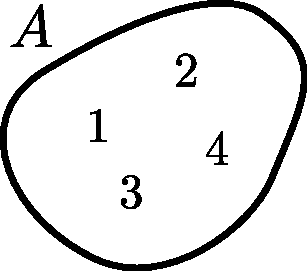
\includegraphics[width=\linewidth]{images/conjA}
\end{image}%
\tcblower
\end{figureptx}%
 e relações de continência (inclusão) entre os conjuntos (por exemplo, \(\{1, 3\} \subset \{1, 2, 3, 4\}\)). Assim, duas curvas que não se tocam e estão uma no espaço interno da outra simbolizam conjuntos que possuem continência; \begin{figureptx}{\(\{1, 3\} \subset \{1, 2, 3, 4\}\).}{x:figure:subconj}{}%
\begin{image}{0.35}{0.3}{0.35}%
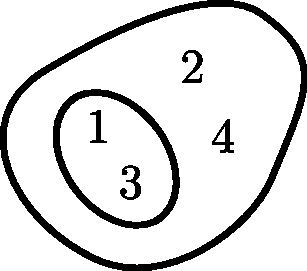
\includegraphics[width=\linewidth]{images/subconj}
\end{image}%
\tcblower
\end{figureptx}%
%
\end{definition}
\begin{definition}{}{g:definition:idp5}%
Sejam \(A_1, A_2, \ldots, A_n\), (\(n\geq 2\)) conjuntos e \(\Omega\) o conjunto universo.%
%
\begin{multicols}{1}
\begin{enumerate}
\item{}O conjunto \emph{união} de \(A_1\) e \(A_2\) é o conjunto dos elementos que pertencem a \(A_1\) ou a \(A_2\). Simbolicamente,%
\begin{equation*}
A_1\cup A_2 = \{ \omega\in\Omega| \omega\in A_1 \text{ ou } \omega\in A_2 \}. 
\end{equation*}
Mais geralmente,%
\begin{equation*}
\bigcup_{i=1}^{n}A_i = A_1\cup \cdots \cup A_n =\{ \omega\in\Omega| \omega\in A_1 \text{ ou } \omega\in A_2 \text{ ou }\cdots \text{ ou } \omega\in A_n \}. 
\end{equation*}
%
\item{}O conjunto \emph{interseção} de \(A_1\) e \(A_2\) é o conjunto dos elementos que pertencem simultaneamente a \(A_1\) e a \(A_2\). Simbolicamente,%
\begin{equation*}
A_1\cap A_2 = \{ \omega\in\Omega| \omega\in A_1 \text{ e } \omega\in A_2 \}. 
\end{equation*}
De forma geral,%
\begin{equation*}
\bigcap_{i=1}^{n}A_i = A_1\cap \cdots \cap A_n =\{ \omega\in\Omega| \omega\in A_1 \text{ e } \omega\in A_2 \text{ e }\cdots \text{ e } \omega\in A_n \}. 
\end{equation*}
%
\item{}Dizemos que \(A_1\) e \(A_2\) são \emph{disjuntos} se \(A_1\cap A_2=\varnothing\). E dizemos que \(A_1, A_2, \ldots, A_n\) são disjuntos quando forem disjuntos dois a dois, ou seja,%
\begin{equation*}
A_i\cap A_j = \varnothing, \text{ para quaisquer } i, j \in\{1, 2, \ldots n\}, \text{ com } i\neq j. 
\end{equation*}
%
\item{}O \emph{conjunto complementar} de \(A_i\) é o conjunto dos elementos de \(\Omega\) que não pertencem a \(A_i\). Simbolicamente%
\begin{equation*}
A_i^c = \{ \omega\in\Omega| \omega\notin A_i \}. 
\end{equation*}
%
\item{}O conjunto \emph{diferença} de \(A_1\) e \(A_2\) é o conjunto dos elementos que pertencem a \(A_1\) e não pertencem a \(A_2\). Simbolicamente,%
\begin{equation*}
A_1\setminus A_2 = A_1\cap A_2^c = \{ \omega\in\Omega | \omega\in A_1 \text{ e } \omega\notin A_2 \}.
\end{equation*}
%
\item{}O \emph{produto cartesiano} de \(A_1\) por \(A_2\) é o conjunto de pares ordenados \((a_1, a_2)\), na qual \(a_1\in A_1\) e \(a_2\in A_2\). Simbolicamente,%
\begin{equation*}
A_1\times A_2 = \{ (a_1, a_2)| a_1\in A_1 \text{ e } a_2\in A_2 \}. 
\end{equation*}
%
\end{enumerate}
\end{multicols}
\end{definition}
\begin{theorem}{}{}{x:theorem:distributiva}%
Sejam \(A, B\) e \(C\) conjuntos; então, valem as seguintes propriedades:%
\begin{enumerate}
\item{}\(\displaystyle A\cap (B\cup C) = (A\cap B)\cup(A\cap C);\)%
\item{}\(\displaystyle A\cup (B\cap C) = (A\cup B)\cap(A\cup C).\)%
\end{enumerate}
%
\end{theorem}
\begin{proof}{}{g:proof:idp6}
Demonstração do item 1:%
\begin{align*}
x\in A\cap(B\cup C) \amp \Leftrightarrow x\in A \text{ e } x\in B\cup C \Leftrightarrow x\in A \text{ e } (x\in B \text{ ou } x\in C) \\
\amp \Leftrightarrow (x\in A \text{ e }x\in B) \text{ ou } (x\in A\text{ e }x\in C) \\
\amp \Leftrightarrow (x\in A\cap B) \text{ ou } (x\in A\cap C) \\
\amp \Leftrightarrow x\in (A\cap B)\cup(A\cap C) 
\end{align*}
%
\par
O segundo pode ser demonstrado de forma análoga.%
\end{proof}
\begin{theorem}{}{}{x:theorem:morgan}%
\emph{(Leis de Morgan)} Sejam \(A\) e \(B\) conjuntos. São válidas as seguintes propriedades:%
\begin{enumerate}
\item{}\(\displaystyle (A \cup B)^c=A^c \cap B^c;\)%
\item{}\(\displaystyle (A \cap B)^c=A^c \cup B^c.\)%
\end{enumerate}
%
\end{theorem}
\begin{proof}{}{g:proof:idp7}
Vamos demonstrar a primeira destas propriedades. A outra é demonstrada de forma análoga. Usamos o fato de que \((A \cup B)^c=A^c \cap B^c\), se, e somente se,  \((A \cup B)^c \subset A^c \cap B^c\) e \(A^c \cap B^c \subset (A \cup B)^c\).%
\par
Seja \(x \in (A \cup B)^c\), logo \(x \notin (A \cup B)\). Sendo assim, \(x \notin A\)  e  \(x \notin B\). Portanto \(x \in A^c\)  e  \(x \in B^c\), logo \(x \in (A^c \cap B^c)\). Acabamos de mostrar que \((A \cup B)^c \subset A^c \cap B^c\).%
\par
Considere \(x \in A^c \cap B^c\), então \(x \in A^c\)  e \(x \in B^c\). Logo \(x \notin A\), \(x \notin B\)  e \(x \notin (A\cap B)\). Portanto, \(x \notin (A \cup B)\), sendo assim \(x \in (A \cup B)^c\). Acabamos de mostrar que \(A^c \cap B^c \subset  (A \cup B)^c\). Portanto%
%
\begin{equation*}
(A \cup \ B)^c=A^c \cap B^c.\qedhere
\end{equation*}
\end{proof}
\end{sectionptx}
\end{chapterptx}
%
%
\typeout{************************************************}
\typeout{Capítulo 2 Princípios de Contagem}
\typeout{************************************************}
%
\begin{chapterptx}{Princípios de Contagem}{}{Princípios de Contagem}{}{}{x:chapter:sets}
\begin{introduction}{}%
Neste Capítulo vamos ver os Princípios Aditivo e Multiplicativo. Em seguida veremos como calcular o número de Permutações e Combinações, dos tipos simples, e tambem com elementos repetidos ou em disposição circular.%
\end{introduction}%
%
%
\typeout{************************************************}
\typeout{Seção 2.1 Princípio Aditivo e Princípio Multiplicativo}
\typeout{************************************************}
%
\begin{sectionptx}{Princípio Aditivo e Princípio Multiplicativo}{}{Princípio Aditivo e Princípio Multiplicativo}{}{}{x:section:section-note-on-proofs}
\begin{objectives}{Objetivos}{x:objectives:objetivos-aditivo-multiplicativo}
%
\begin{enumerate}
\item{}Definir o Princípio Aditivo.%
\item{}Definir o Princípio Multiplicativo.%
\item{}Exemplificar.%
\end{enumerate}
\end{objectives}
\begin{introduction}{}%
\begin{remark}{}{g:remark:idp8}%
Usaremos o símbolo \(\#A\) para representar o número de elementos do conjunto \(A\), isto é, a cardinalidade de \(A\).%
\par
Dizemos que dois conjuntos \(A\) e \(B\) são disjuntos quando \(A\cap B=\emptyset\).%
\end{remark}
\end{introduction}%
%
%
\typeout{************************************************}
\typeout{Subseção 2.1.1 Princípio Aditivo}
\typeout{************************************************}
%
\begin{subsectionptx}{Princípio Aditivo}{}{Princípio Aditivo}{}{}{g:subsection:idp9}
\begin{example}{}{g:example:idp10}%
Suponha que na disciplina de análise combinatória existem três listas de exercício. A 1ª contém 15 exercícios, a 2ª contém 18 exercícios e a 3ª contém 14 exercícios. De quantas maneiras um estudante pode escolher um exercício para resolver?%
\end{example}
\textbf{\blocktitlefont Solução}.\quad{}O estudante têm 15 opções para escolher um exercício da primeira lista, 18 opções para escolher um exercício da segunda lista e 14 opções para escolher um exercício da terceira lista. Portanto o estudante têm%
\begin{equation*}
15+18+14 = 47
\end{equation*}
maneiras de escolher um exercício.%
\begin{definition}{}{g:definition:idp11}%
\terminology{(O Princípio Aditivo 1ª versão)} Se uma tarefa puder ser feita de \(n_1\) maneiras e uma segunda tarefa de \(n_2\) maneiras e se essas tarefas não puderem ser feitas ao mesmo tempo; então, existem \(n_1+n_2\) maneiras de fazer ambas as tarefas.%
\end{definition}
\begin{theorem}{}{}{g:theorem:idp12}%
\terminology{(O Princípio Aditivo 2ª versão)} Sejam \(A\) e \(B\) conjuntos finitos e disjuntos, então%
\begin{equation*}
\#(A\cup B)=\#A+ \#B
\end{equation*}
%
\end{theorem}
\begin{proof}{}{g:proof:idp13}
Sejam \(T_a\) e \(T_b\) as tarefas de escolher um elemento em \(A\) e em \(B\), respectivamente. Existem \(\#A\) maneiras de escolher um elemento em \(A\) e \(\#B\) maneiras de escolher um elemento em \(B\). Pelo Princípio Aditivo 1ª versão, como as tarefas não podem ser feitas ao mesmo tempo, o número de maneiras de escolher um elemento em cada um dos conjuntos é%
\begin{equation*}
\#(A\cup B)=\#A+ \#B.\qedhere
\end{equation*}
%
\end{proof}
\begin{technology}{}{g:technology:idp14}%
Abaixo, clique em "Evaluate (Sage)" para obter a lista com todos os elementos da união dos conjuntos \(\{a, b, c\}\) e \(\{1, 2, 3, 4\}\).%
\begin{sageinput}
['a', 'b', 'c']+[1, 2, 3, 4]
\end{sageinput}
\begin{sageoutput}
['a', 'b', 'c', 1, 2, 3, 4]
\end{sageoutput}
\end{technology}
\end{subsectionptx}
%
%
\typeout{************************************************}
\typeout{Subseção 2.1.2 Princípio Multiplicativo}
\typeout{************************************************}
%
\begin{subsectionptx}{Princípio Multiplicativo}{}{Princípio Multiplicativo}{}{}{g:subsection:idp15}
\begin{fact}{}{}{g:fact:idp16}%
Quantos números naturais de três algarismos distintos (na base 10) existem?%
\textbf{\blocktitlefont Solução}.\quad{}O procedimento de escolher um número satisfazendo estas hipóteses pode ser quebrado em três tarefas.%
\begin{enumerate}
\item{}A 1ª tarefa é escolher o primeiro dígito, (da esquerda para a direita) que pode ser feito de 9 maneiras, já que o zero não pode ser escolhido.%
\item{}A 2ª tarefa é escolher o segundo dígito, que pode ser feito de 9 maneiras, pois não pode ser igual a escolha do primeiro dígito.%
\item{}A 3ª tarefa é escolher o terceiro dígito, que pode ser feito de 8 maneiras, pois não pode ser igual aos dois primeiros dígitos.%
\end{enumerate}
A resposta é%
\begin{equation*}
9\times 9\times 8 = 648\text{.}
\end{equation*}
%
\end{fact}
\begin{definition}{}{g:definition:idp17}%
\terminology{(O Princípio Multiplicativo 1ª versão)} Suponha que um procedimento pode ser quebrado em duas tarefas. Se existem \(n_1\) maneiras de executar a primeira tarefa e \(n_2\) maneiras de executar a segunda tarefa, depois que a primeira tarefa estiver executada, então existem \(n_1\times n_2\) maneiras de executar o procedimento.%
\end{definition}
\begin{theorem}{}{}{g:theorem:idp18}%
\terminology{(Princípio Multiplicativo 2ª versão)} Sejam \(A\) e \(B\) conjuntos finitos; então,%
\begin{equation*}
\#(A\times B) = \#A\times \#B.
\end{equation*}
%
\end{theorem}
\begin{proof}{}{g:proof:idp19}
Note que a tarefa de escolher um elemento no produto cartesiano \(A\times B\) pode ser feita escolhendo um elemento em \(A\) e um elemento em \(B\), do Princípio Multiplicativo 1ª versão temos%
\begin{equation*}
\#(A\times B) = \#A\times \#B.\qedhere
\end{equation*}
%
\end{proof}
\begin{technology}{}{g:technology:idp20}%
Abaixo, clique em "Evaluate (Sage)" para obter a lista com todos os elementos do produto cartesiano \(\{a, b, c\}\times\{1, 2, 3\}\).%
\begin{sageinput}
cartesian_product([['a', 'b', 'c'],[1, 2, 3]]).list()
\end{sageinput}
\begin{sageoutput}
[('a', 1),
 ('a', 2),
 ('a', 3),
 ('b', 1),
 ('b', 2),
 ('b', 3),
 ('c', 1),
 ('c', 2),
 ('c', 3)]
\end{sageoutput}
\end{technology}
\begin{fact}{}{}{g:fact:idp21}%
A placa dos automóveis eram formadas por 3 letras (K, Y e W inclusive) seguidas por quatro algarismos. Quantas placas podiam ser formadas?%
\textbf{\blocktitlefont Solução}.\quad{}Cada letra pode ser escolhida de 26 modos e cada algarismo de 10 modos distintos. A resposta é%
\begin{equation*}
26\times26\times26\times 10\times10\times10\times10 = 26^3\times10^4 = 175760000.
\end{equation*}
%
\end{fact}
\begin{fact}{}{}{g:fact:idp22}%
Sejam \(A\) e \(B\) dois conjuntos com \(\#A=m\) e \(\#B=n\).%
\begin{enumerate}
\item{}Quantas são as funções \(f:A\rightarrow B?\)%
\item{}Quantas são as funções injetoras \(f:A\rightarrow B?\)%
\end{enumerate}
%
\textbf{\blocktitlefont Solução}.\quad{}\terminology{Solução} 1. Devemos escolher a imagem de cada elemento de \(A\). Existem \(n\) modos de escolher a imagem do "primeiro" elemento de \(A\), \(n\) modos de escolher a imagem do "segundo" elemento de \(A\) \(\ldots\) até \(n\) modos de escolher a imagem do "m-ésimo" elemento de \(A\). Pelo princípio multiplicativo, temos%
\begin{equation*}
\overbrace{n\times n \times n \cdots \times n}^{m \text{ termos}} = n^m. 
\end{equation*}
2. Primeiramente, para existir solução precisamos que \(n\geq m\), pois a função precisa ser injetora. Neste caso, existem \(n\) modos de escolher a imagem do "primeiro" elemento de \(A\), \(n-1\) modos de escolher a imagem do "segundo" elemento de \(A\) \(\ldots\) até \(n-m+1\) modos de escolher a imagem do "m-ésimo" elemento de \(A\). A resposta é%
\begin{equation*}
(n-0)\times(n-1)\times(n-2)\times \cdots \times(n-(m-1))  
\end{equation*}
%
\end{fact}
\begin{fact}{}{}{g:fact:idp23}%
Quantos são os números naturais pares que se escrevem (na base 10) com três algarismos distintos?%
\textbf{\blocktitlefont Solução}.\quad{}Já sabemos que o número total de números naturais com três algarismos distintos é%
\begin{equation*}
9\times 9\times 8 = 648. 
\end{equation*}
Podemos contar dentre estes, os que são ímpares, a diferença será a resposta deste problema. O último algarismo pode ser escolhido de 5 maneiras (1, 3, 5, 7 ou 9). O primeiro algarismo pode ser escolhido de 8 maneiras (não pode ser o zero, nem o que foi escolhido para o último algarismo) e o segundo algarismo pode ser escolhido de 8 maneiras (nem pode ser igual ao primeiro nem ao último). Portanto a resposta é%
%
\begin{equation*}
648 - 5\times 8\times 8=328. 
\end{equation*}
%
\end{fact}
\end{subsectionptx}
%
%
\typeout{************************************************}
\typeout{Exercícios 2.1.3 Exercícios}
\typeout{************************************************}
%
\begin{exercises-subsection}{Exercícios}{}{Exercícios}{}{}{g:exercises:idp24}
\begin{divisionexercise}{1}{}{}{g:exercise:idp25}%
Quantas palavras contendo 5 letras diferentes podem ser formadas com um alfabeto de 26 letras?%
\par\smallskip%
\noindent\textbf{\blocktitlefont Resposta}.\hypertarget{g:answer:idp26}{}\quad{}26×25×24×23×22=7893600%
\end{divisionexercise}%
\begin{divisionexercise}{2}{}{}{g:exercise:idp27}%
Quantos são os gabaritos possíveis de um teste de 25 questões de múltipla-escolha, com cinco alternativas por questão?%
\par\smallskip%
\noindent\textbf{\blocktitlefont Resposta}.\hypertarget{g:answer:idp28}{}\quad{}\(5^{25}=298023223876953125\)%
\end{divisionexercise}%
\begin{divisionexercise}{3}{}{}{g:exercise:idp29}%
Quantos divisores naturais possui o número 600?%
\par\smallskip%
\noindent\textbf{\blocktitlefont Resposta}.\hypertarget{g:answer:idp30}{}\quad{}4×2×3=24%
\end{divisionexercise}%
\begin{divisionexercise}{4}{}{}{g:exercise:idp31}%
Em uma banca há 7 exemplares iguais da revista A, 4 exemplares iguais da revista B e 15 exemplares igauis da revista C. Quantas coleções não vazias de revistas dessa banca é possível formar?%
\par\smallskip%
\noindent\textbf{\blocktitlefont Resposta}.\hypertarget{g:answer:idp32}{}\quad{}8×5×16−1=639%
\end{divisionexercise}%
\begin{divisionexercise}{5}{}{}{g:exercise:idp33}%
Quantos números inteiros entre 1000 e 9999 são ímpares e possuem quatro dígitos distintos?%
\par\smallskip%
\noindent\textbf{\blocktitlefont Resposta}.\hypertarget{g:answer:idp34}{}\quad{}5×8×8×7=2240%
\end{divisionexercise}%
\end{exercises-subsection}
\end{sectionptx}
%
%
\typeout{************************************************}
\typeout{Seção 2.2 Permutações Simples}
\typeout{************************************************}
%
\begin{sectionptx}{Permutações Simples}{}{Permutações Simples}{}{}{x:section:section-permutacoes-simples}
\begin{objectives}{Objetivos}{x:objectives:objetivos-permutacoes-simples}
%
\begin{enumerate}
\item{}Nota histórica%
\item{}Definir Permutação Simples.%
\item{}Mostrar como obter a lista com todas as permutações de \(n\) elementos distintos no Sage.%
\item{}Mostrar como calcular o número de permutações com \(n\) elementos distintos.%
\item{}Exemplificar.%
\end{enumerate}
\end{objectives}
%
%
\typeout{************************************************}
\typeout{Subseção 2.2.1 Nota Histórica}
\typeout{************************************************}
%
\begin{subsectionptx}{Nota Histórica}{}{Nota Histórica}{}{}{g:subsection:idp35}
Al-Khalil (717-786), um matemático e criptógrafo árabe, escreveu o Livro de Mensagens Criptográficas. Ele contém o primeiro uso de permutações e combinações, para listar todas as palavras árabes possíveis com e sem vogais.%
\par
A regra para determinar o número de permutações de \(n\) objetos era conhecida na cultura indiana por volta de 1150. O Lilavati, do matemático indiano Bhaskara II, contém uma passagem que se traduz em:%
\begin{quote}%
\emph{O produto da multiplicação da série aritmética começando e aumentando pela unidade e continuando até o número de casas, serão as variações do número com algarismos específicos.}\end{quote}
Fonte: \href{https://en.wikipedia.org/wiki/Permutation}{\terminology{en.wikipedia.org\slash{}wiki\slash{}Permutation}}.%
\end{subsectionptx}
%
%
\typeout{************************************************}
\typeout{Subseção 2.2.2 Permutações}
\typeout{************************************************}
%
\begin{subsectionptx}{Permutações}{}{Permutações}{}{}{g:subsection:idp36}
Permutar uma lista de objetos é mudar a ordem em que os objetos da lista aparecem originalmente.%
\par
Abaixo, temos uma lista com todas as permutações dos elementos: 1, 2, 3.%
\par
[[1, 2, 3], [1, 3, 2], [2, 1, 3], [2, 3, 1], [3, 1, 2], [3, 2, 1]]%
\begin{technology}{}{g:technology:idp37}%
Abaixo, clique em "Evaluate (Sage)" para obter a lista com todas as permutações dos elementos: 1, 2, 3, 4.%
\begin{sageinput}
Permutations([1, 2, 3, 4]).list()
\end{sageinput}
\begin{sageoutput}
[[1, 2, 3, 4],
 [1, 2, 4, 3],
 [1, 3, 2, 4],
 [1, 3, 4, 2],
 [1, 4, 2, 3],
 [1, 4, 3, 2],
 [2, 1, 3, 4],
 [2, 1, 4, 3],
 [2, 3, 1, 4],
 [2, 3, 4, 1],
 [2, 4, 1, 3],
 [2, 4, 3, 1],
 [3, 1, 2, 4],
 [3, 1, 4, 2],
 [3, 2, 1, 4],
 [3, 2, 4, 1],
 [3, 4, 1, 2],
 [3, 4, 2, 1],
 [4, 1, 2, 3],
 [4, 1, 3, 2],
 [4, 2, 1, 3],
 [4, 2, 3, 1],
 [4, 3, 1, 2],
 [4, 3, 2, 1]]
\end{sageoutput}
Os números podem ser alterados, ao executar o código, a lista das permutações será atualizada.%
\end{technology}
Para descrever o \emph{número de permutações} de \(n\) objetos distintos usamos a notação: \(P_n\) ou \(P(n)\).%
\begin{theorem}{}{}{g:theorem:idp38}%
O número de permutações de \(n \) objetos distintos é%
\begin{equation*}
P_n = P(n) = n\times (n-1) \times (n-2)\times \cdots \times 1. 
\end{equation*}
\end{theorem}
\begin{proof}{}{g:proof:idp39}
Pelo princípio multiplicativo, temos \(n\) modos de escolher o elemento que ocupará o primeiro lugar, uma vez tomada essa decisão, teremos \(n-1\) modos de se escolher o segundo, e assim por diante, até que haja apenas um único modo de se escolher o último elemento. Portanto%
\begin{equation*}
P(n) = n\times (n-1) \times \cdots \times 1. \qedhere
\end{equation*}
%
\end{proof}
\begin{fact}{}{}{g:fact:idp40}%
Quantos são os anagramas da palavra SAGE?%
\textbf{\blocktitlefont Solução}.\quad{}A palavra SAGE possui quatro letras distintas, potanto o número de anagramas é%
\begin{equation*}
P(4) = 24. 
\end{equation*}
%
\end{fact}
\begin{fact}{}{}{g:fact:idp41}%
Quantos são os anagramas da palavra XADREZ que começam e terminam por consoante?%
\textbf{\blocktitlefont Solução}.\quad{}A consoante inicial pode ser escolhida de 4 maneiras e a consoante final de 3 maneiras e as 4 letras restantes podem ser escolhidas de \(P(4)\) maneiras. A resposta é%
\begin{equation*}
4\times 3\times P(4). 
\end{equation*}
%
\begin{sageinput}
4*3*factorial(4)
\end{sageinput}
\begin{sageoutput}
288
\end{sageoutput}
\end{fact}
\begin{fact}{}{}{g:fact:idp42}%
De quantos modos podemos dividir 12 pessoas em três grupos de quatro pessoas cada?%
\textbf{\blocktitlefont Solução}.\quad{}Podemos colocar as 12 pessoas em uma fila. O primeiro grupo será formado pelas 4 primeiras pessoas, o segundo grupo, pelas 4 pessoas seguintes e o terceiro grupo pelas quatro últimas pessoas. O número total de formas de ordenar as 12 pessoas é P(12). Como a separação em grupos%
\begin{equation*}
[1, 2, 3, 4], [5, 6, 7, 8], [9, 10, 11, 12]
\end{equation*}
é idêntica a separação%
\begin{equation*}
[9, 10, 11, 12], [1, 2, 3, 4], [5, 6, 7, 8]
\end{equation*}
A contagem P(12) foi contada como se fossem distintas, precismos dividir pelo número de formas de ordenar os três grupos e precisamos dividir também pelo número de formas de ordenar cada grupo. Portanto a resposta é%
\begin{equation*}
\frac{P(12)}{P(3)\times P(4)\times P(4)\times P(4)}.
\end{equation*}
%
\begin{sageinput}
P(n) = factorial(n)
P(12)/(P(3)*P(4)*P(4)*P(4))
\end{sageinput}
\begin{sageoutput}
5775
\end{sageoutput}
\end{fact}
\begin{fact}{}{}{g:fact:idp43}%
Permutam-se de todos os modos possíveis os algarismos 2, 3, 5, 6, 8, 9 e escrevem-se os números assim formados em ordem crescente.%
%
\begin{enumerate}
\item{}Que lugar ocupa o número 653289?%
\item{}Qual o número que ocupa o 500º lugar?%
\end{enumerate}
\textbf{\blocktitlefont Solução}.\quad{}\terminology{item 1.}%
\par
Os números que começam com 2, 3 e 5 aparecem antes do número 653289. Existem \(5!\) números que começam com cada um destes algarismos, ou seja \(3\times 5!\) números.%
\par
Existem \(4!\) números que começam com 62 e a mesma quantidade que começam com 63, ou seja \(2\times 4!\) números.%
\par
Existem \(3!\) números que começam com 652.%
\par
O próximo números já que o que queremos. Portanto a resposta é%
\begin{equation*}
3\times 5! + 2\times 4! +3! +1 = 415.
\end{equation*}
%
\par
\terminology{item 2.}%
\par
Os números que começam com 2, 3, 5 e 6 dão um total de \(4\times 5! = 480\) números. Se considerarmos também, todos que começam com 8, teremos mais 120 números, ultrapassando a posição 500.%
\par
Já sabemos que o número que ocupa a posição 500 começa com o algarismo 8 e que o primeiro número com o algarismo 8 ocupa a posição 481. Precisamos encontrar o número que começa com o algarismo 8 e está na posição 20, dentre estes números que começam com 8.%
\par
Começando com 823, 825 e 826, temos \(3\times 3! = 6\) números. Dessa forma o número seguinte está na posição 19, começando com o algarismo 8. Então o número 829356 está na posição 499 e o número 829365 está na posição 500.%
\par
\terminology{(Usando o Sage)}%
\par
Quando calculamos todas as permutações no Sage, a saída é exibida em ordem crescente. Como as listas no Sage\slash{}Python começam a ser contadas a partir do zero, podemos consultar a permutação de posição 500 com o comando abaixo:%
\begin{sageinput}
Permutations([2, 3, 5, 6, 8, 9]).list()[499]
\end{sageinput}
\begin{sageoutput}
[8, 2, 9, 3, 6, 5]
\end{sageoutput}
\end{fact}
\end{subsectionptx}
%
%
\typeout{************************************************}
\typeout{Exercícios 2.2.3 Exercícios}
\typeout{************************************************}
%
\begin{exercises-subsection}{Exercícios}{}{Exercícios}{}{}{g:exercises:idp44}
\begin{divisionexercise}{1}{}{}{g:exercise:idp45}%
Quantos são os anagramas da palavra SINGULAR:%
%
\begin{multicols}{1}
\begin{enumerate}[label=(\alph*)]
\item{}Que começam por consoante e terminam por vogal?%
\item{}Que têm as letras S,I,N juntas em qualquer ordem?%
\item{}Que têm as vogais e as consoantes intercaladas?%
\end{enumerate}
\end{multicols}
\par\smallskip%
\noindent\textbf{\blocktitlefont Resposta}.\hypertarget{g:answer:idp46}{}\quad{}a) 5×3×6!=10800, b) \(3!\times 6!=4320\), c) 0%
\end{divisionexercise}%
\begin{divisionexercise}{2}{}{}{g:exercise:idp47}%
De quantos modos é possível sentar 12 pessoas em cadeiras em fila de modo que três determinadas pessoas dessas 12 não fiquem juntas?%
\par\smallskip%
\noindent\textbf{\blocktitlefont Resposta}.\hypertarget{g:answer:idp48}{}\quad{}12!−3!×10!%
\end{divisionexercise}%
\begin{divisionexercise}{3}{}{}{g:exercise:idp49}%
Quantos dados diferentes podemos formar gravando números de 1 a 6 sobre as faces indistinguíveis de um cubo?%
\par\smallskip%
\noindent\textbf{\blocktitlefont Resposta}.\hypertarget{g:answer:idp50}{}\quad{}\(\frac{6!}{6\times 4} = 30 \)%
\end{divisionexercise}%
\begin{divisionexercise}{4}{}{}{g:exercise:idp51}%
Permutam-se de todos os modos possíveis os algarismos 1, 2, 3, 5, 6, 8 e escrevem-se os números assim formados em ordem crescente.%
\par
a) Que lugar ocupa o número 653812?%
\par
b) Qual o número que ocupa o 110º lugar?%
\par
c) Qual a soma dos números assim formados?%
\par\smallskip%
\noindent\textbf{\blocktitlefont Resposta}.\hypertarget{g:answer:idp52}{}\quad{}a) 569, b) 185263, c) 356000040%
\end{divisionexercise}%
\begin{divisionexercise}{5}{}{}{g:exercise:idp53}%
\terminology{(OPEMAT - 2019 - nível 1)} Em uma viagem a Recife, o grupo formado pelos números 1, 2, 3, 4 e 5, resolveu tirar fotos próximo ao monumento do Parque das Esculturas do artista Pernambucano Francisco Brennand. Indecisos pela escolha da disposição na foto, eles concordaram em tirar várias fotos em todas as disposições possíveis, permutando os lugares entre si conforme as imagens abaixo (\hyperref[x:figure:Brennand]{Figura~{\xreffont\ref{x:figure:Brennand}}}):%
\begin{figureptx}{}{x:figure:Brennand}{}%
\begin{image}{0.05}{0.9}{0.05}%
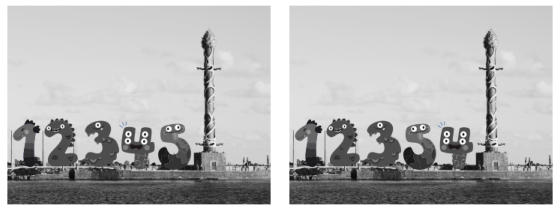
\includegraphics[width=\linewidth]{images/Brennand}
\end{image}%
\tcblower
\end{figureptx}%
Por fim, eles colocaram as fotos em ordem crescente de numeração formando a seguinte lista:%
%
\begin{equation*}
1 2 3 4 5 , 1 2 3 5 4 , 1 2 4 3 5 , \ldots , 5 4 3 1 2 , 5 4 3 2 1
\end{equation*}
Julgue as afirmações a seguir atribuindo (V) se a afirmação for verdadeira e (F) se a afirmação for falsa.%
\par
\terminology{A} – (V) (F) Quem ocupa a última posição da vigésima foto é o 3.%
\par
\terminology{B} – (V) (F) A foto em que os números aparecem na disposição 32541, ocupa o 59º lugar desta lista.%
\par
\terminology{C} – (V) (F) A quantidade de fotos em que os números 1 e 2 aparecem separados é 96.%
\par
\terminology{D} – (V) (F) A quantidade de fotos em que a disposição dos números é maior do que a foto com disposição 25413 é 73.%
\par
\terminology{E} – (V) (F) A soma de todos os números de cinco dígitos representados pelas fotos é 3999960.%
\par\smallskip%
\noindent\textbf{\blocktitlefont Resposta}.\hypertarget{g:answer:idp54}{}\quad{}A) V, B) F, C) F, D) V, E) V%
\end{divisionexercise}%
\end{exercises-subsection}
\end{sectionptx}
%
%
\typeout{************************************************}
\typeout{Seção 2.3 Combinações Simples}
\typeout{************************************************}
%
\begin{sectionptx}{Combinações Simples}{}{Combinações Simples}{}{}{x:section:section-combinacoes-simples}
\begin{objectives}{Objetivos}{x:objectives:objetivos-combinacao-simples}
%
\begin{enumerate}
\item{}Definir combinação simples.%
\item{}Mostrar como obter a lista com todas as combinações simples de \(n\) elementos distintos, tomados \(p\) a \(p\) no Sage.%
\item{}Mostrar como calcular o número de combinações simples de \(n\) elementos distintos, tomados \(p\) a \(p\).%
\item{}Exemplificar.%
\end{enumerate}
\end{objectives}
%
%
\typeout{************************************************}
\typeout{Subseção 2.3.1 Combinações}
\typeout{************************************************}
%
\begin{subsectionptx}{Combinações}{}{Combinações}{}{}{g:subsection:idp55}
\begin{fact}{}{}{g:fact:idp56}%
Quantas saladas contendo exatamente 7 frutas podemos formar se dispomos de 12 frutas diferentes?%
\textbf{\blocktitlefont Solução}.\quad{}Para a 1ª fruta, temos 12 opções de escolha, para a 2ª fruta, temos 11 opções de escolha, \(\dots\) para a 7ª fruta temos, 6 opções de escolha. Como a ordem não importa, precisamos dividir pelo número de maneiras de ordenar estas frutas. Portanto a resposta é%
\begin{equation*}
\frac{12\times 11\times 10\times \cdots \times 6}{P(7)}.
\end{equation*}
%
\begin{sageinput}
(12*11*10*9*8*7*6)/factorial(7)
\end{sageinput}
\begin{sageoutput}
792
\end{sageoutput}
\end{fact}
\begin{definition}{}{g:definition:idp57}%
O número de \emph{combinações simples} de \(n\) objetos, tomados \(p\) a \(p\) é o número de modos de escolher \(p\) objetos distintos entre \(n\) objetos distintos dados.%
\par
Outra forma de definir \emph{combinações simples} de \(n\), \(p\) a \(p\) é como o número de subconjuntos com \(p\) elementos de um conjunto com \(n\) elementos. A notação para combinação simples é dada por%
\begin{equation*}
C_n^p, C_{n, p} ~~\text{ ou }~~ C(n, p).
\end{equation*}
%
\end{definition}
\begin{technology}{}{g:technology:idp58}%
No Sage, podemos obter uma lista com todos os subconjuntos de \textbraceleft{}1, 2, 3, 4, 5\textbraceright{}, tomados 3 a 3. Basta usar o seguinte código:%
\begin{sageinput}
Combinations([1, 2, 3, 4, 5], 3).list()
\end{sageinput}
\begin{sageoutput}
[[1, 2, 3],
 [1, 2, 4],
 [1, 2, 5],
 [1, 3, 4],
 [1, 3, 5],
 [1, 4, 5],
 [2, 3, 4],
 [2, 3, 5],
 [2, 4, 5],
 [3, 4, 5]]
\end{sageoutput}
\end{technology}
\begin{theorem}{}{}{g:theorem:idp59}%
O número de combinações de \(n\) objetos distintos, tomados \(p \) a \(p \) é%
\begin{equation*}
C_n^p = \frac{n!}{p!\times(n-p)!}. 
\end{equation*}
\end{theorem}
\begin{proof}{}{g:proof:idp60}
Temos \(n\) modos de escolher o primeiro elemento, \(n-1\) modos de escolher o segundo elemento, e assim sucessivamente, até \(n-p+1\) modos de escolher o \(p\)-ésimo elemento.%
\par
Agora observe que contamos muito mais agrupamentos do que deveríamos, pois para conjuntos, a ordem não importa, portanto precisamos dividir pelo número de formas de ordenar estes \(p\) elementos que escolhemos de forma ordenada, ou seja, por \(p!\). Assim:%
\par
%
\begin{equation*}
C(n,p)  = \frac{n(n-1)\cdots(n-p+1)}{p!} = \frac{n(n-1)\cdots(n-p+1)}{p!} \cdot \frac{(n-p)!}{(n-p)!}
\end{equation*}
%
\par
Fazendo as contas concluímos que%
\begin{equation*}
C(n,p) = \frac{n!}{p!(n-p)!}.\qedhere
\end{equation*}
%
\end{proof}
\begin{technology}{}{g:technology:idp61}%
Para obter o número de \emph{combinações simples} de \(n\), tomados \(p\) a \(p\),usamos o código binomial(n, p). Teste o código abaixo, para o caso \(n=8\), \(p=3\).%
\begin{sageinput}
binomial(8,3)
\end{sageinput}
\begin{sageoutput}
56
\end{sageoutput}
\end{technology}
\begin{fact}{}{}{g:fact:idp62}%
Sobre uma reta, marcam-se 10 pontos e sobre outra reta paralela a primeira marcam-se 15 pontos. Quantos triângulos podemos obter unindo 3 desses 25 pontos?%
\textbf{\blocktitlefont Solução}.\quad{}Para formar um triângulo precisamos escolher dois vértices em uma das retas e um vértice na outra reta.%
\par
O número de formas de escolher dois vértices na primeira reta é \(C(10, 2)\) uma vez tomada esta decisão precisamos escolher um vértice na segunda reta, isto pode ser feito de 15 maneiras. O total de formas de formar um triângulo com dois vértices na primeira reta é:%
\begin{equation*}
15\times C(10, 2). 
\end{equation*}
%
\par
Com a mesma ideia, o número de formas de formar um triângulo com dois vértices na segunda reta é%
\begin{equation*}
10\times C(15, 2). 
\end{equation*}
%
\par
Portanto, pelo princípio aditivo, o número total de soluções é:%
\begin{equation*}
15\times C(10, 2) + 10\times C(15, 2). 
\end{equation*}
%
\begin{sageinput}
C(n, p) = binomial(n, p)
15*C(10, 2) + 10*C(15, 2)
\end{sageinput}
\begin{sageoutput}
1725
\end{sageoutput}
\end{fact}
\begin{fact}{}{}{g:fact:idp63}%
Um Juiz dispõe de 11 pessoas, das quais somente 4 são advogados.%
\par
a) Para formar um único júri com 9 jurados. Qual é o número de formas de compor o júri, com pelo menos 2 advogados?%
\par
b) Para formar um único júri com 6 jurados. Qual é o número de formas de compor o júri, com pelo menos 2 advogados?%
\textbf{\blocktitlefont Solução}.\quad{}\terminology{a)} Basta escolher 9 jurados, pois pelo menos duas serão advogados. O que pode ser feito de%
\begin{equation*}
C(11,9)=55. 
\end{equation*}
%
\par
\terminology{b)} Se escolhermos diretamente 6 jurados, dentre as 11 pessoas disponíveis, pode aconteder de não termos pelo menos dois advogados. Precisamos contornar este problema.%
\par
Precisamos escolher 2 advogados e 4 não advogados, depois 3 advogados e 3 não advogados e por último, precisamos escolher 4 advogados e 2 não advogados. O que pode ser feito de%
\begin{equation*}
C(4,2)\times C(7, 4) + C(4,3)\times C(7, 3) + C(4,4)\times C(7, 2). 
\end{equation*}
maneiras.%
\begin{sageinput}
C(n, p) = binomial(n, p)
C(4,2)*C(7, 4) + C(4,3)*C(7, 3) + C(4,4)*C(7, 2)
\end{sageinput}
\begin{sageoutput}
371
\end{sageoutput}
\end{fact}
\begin{fact}{}{}{g:fact:idp64}%
De quantos modos podemos dividir 12 pessoas em três grupos de quatro pessoas cada?%
\textbf{\blocktitlefont Solução}.\quad{}Para o primeiro grupo, temos um total de%
\begin{equation*}
C(12, 4) 
\end{equation*}
maneiras de selecionar as 4 pessoas. Para o segundo grupo temos um total de%
\begin{equation*}
C(8, 4) 
\end{equation*}
maneiras de selecionar as 4 pessoas. Para o terceiro grupo temos um total de%
\begin{equation*}
C(4,4) 
\end{equation*}
maneiras de selecionar as 4 pessoas. Como a ordem dos grupos não importa, precisamos dividir por \(3!\) Portanto a resposta é%
\begin{equation*}
\frac{C(12, 4)\times C(8, 4)\times C(4, 4)}{3!}.
\end{equation*}
%
\begin{sageinput}
C(n, p) = binomial(n, p)
P(n) = factorial(n)
C(12, 4)*C(8,4)*C(4, 4)/P(3)
\end{sageinput}
\begin{sageoutput}
5775
\end{sageoutput}
\end{fact}
\end{subsectionptx}
%
%
\typeout{************************************************}
\typeout{Exercícios 2.3.2 Exercícios}
\typeout{************************************************}
%
\begin{exercises-subsection}{Exercícios}{}{Exercícios}{}{}{g:exercises:idp65}
\begin{divisionexercise}{1}{}{}{g:exercise:idp66}%
Quantas diagonais possuem um polígono de \(n\) lados?%
\par\smallskip%
\noindent\textbf{\blocktitlefont Resposta}.\hypertarget{g:answer:idp67}{}\quad{}\(\frac{n(n-3)}{2} \)%
\end{divisionexercise}%
\begin{divisionexercise}{2}{}{}{g:exercise:idp68}%
De quantos modos 20 jogados podem ser divididos em 4 times de futsal de 5 jogadores cada, denomidados Sport, Náutico, Santa Cruz e Salgueiro?%
\par\smallskip%
\noindent\textbf{\blocktitlefont Resposta}.\hypertarget{g:answer:idp69}{}\quad{}\(C_{20}^5\times C_{15}^5\times C_{10}^5\times 1 = 11732745024 \)%
\end{divisionexercise}%
\begin{divisionexercise}{3}{}{}{g:exercise:idp70}%
De uma turma formada por 12 homens e 8 mulheres, dentre eles Ana e Bruno, deseja-se formar uma comissão de 10 membros. Quantas são as opções que temos de escolher os membros para formar esta comissão:%
%
\begin{multicols}{1}
\begin{enumerate}[label=(\alph*)]
\item{}sem restrições?%
\item{}de modo que sejam escolhidas 5 pessoas de cada sexo?%
\item{}de modo que sejam escolhidas 5 pessoas de escolhidas?%
\item{}escolhendo-se 5 pessoas de cada sexo, dentre elas Ana e Bruno?%
\item{}de modo que sejam escolhidas 5 pessoas de cada sexo, sendo que Ana e Bruno não sejam escolhidos?%
\item{}de modo que sejam escolhidas 5 pessoas de cada sexo, sendo que se Ana for escolhida, então Bruno não deverá participar?%
\end{enumerate}
\end{multicols}
\par\smallskip%
\noindent\textbf{\blocktitlefont Resposta}.\hypertarget{g:answer:idp71}{}\quad{}%
\begin{multicols}{1}
\begin{enumerate}[label=(\alph*)]
\item{}\(\displaystyle C_{20}^{10} = 184756\)%
\item{}\(\displaystyle C_8^5\times C_{12}^5 = 44352 \)%
\item{}\(\displaystyle C_1^1\times C_7^4\times C_12^5 = 27720 \)%
\item{}\(\displaystyle 1\times 25\times 1\times 330 = 11550 \)%
\item{}\(\displaystyle C_7^5\times C_11^5 = 21\times 462 = 9702 \)%
\item{}\(\displaystyle 32802 \)%
\end{enumerate}
\end{multicols}
\end{divisionexercise}%
\end{exercises-subsection}
\end{sectionptx}
%
%
\typeout{************************************************}
\typeout{Seção 2.4 Permutações Circulares}
\typeout{************************************************}
%
\begin{sectionptx}{Permutações Circulares}{}{Permutações Circulares}{}{}{x:section:section-permutacoes-circulares}
\begin{objectives}{Objetivos}{x:objectives:objetivos-permutacoes-circulares}
%
\begin{enumerate}
\item{}Definir Permutação Circular.%
\item{}Mostrar como obter a lista com todas as permutações circulares com \(n\) elementos distintos no Sage.%
\item{}Mostrar como calcular o número de permutações circulares de \(n\) elementos distintos.%
\item{}Exemplificar.%
\end{enumerate}
\end{objectives}
\begin{definition}{}{g:definition:idp72}%
O número de \emph{permutações circulares} de \(n\) elementos, é o número de maneiras de organizar \(n\) objetos distintos ao longo de um círculo fixo (isto é, não pode ser retirado do plano e virado). Notação:%
\begin{equation*}
PC_n ~~\text{ ou }~~ PC(n). 
\end{equation*}
%
\end{definition}
\begin{remark}{}{g:remark:idp73}%
Observe que os três circulos da  (\hyperref[x:figure:circ-equiv]{Figura~{\xreffont\ref{x:figure:circ-equiv}}}) são equivalentes, ou seja, representam a mesma permutação circular, pois o segundo círculo pode ser obtido a partir do primeiro por uma rotação de \(-\frac{2\pi}{3}\) e o terceiro círculo pode ser obtido a partir do primeiro por uma rotação de \(-2\times\frac{2\pi}{3}\).%
\begin{figureptx}{Três circulos que representam a mesma permutação circular.}{x:figure:circ-equiv}{}%
\begin{image}{0}{1}{0}%
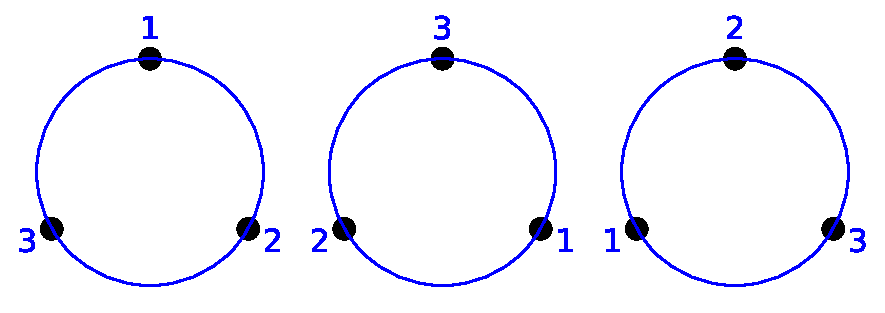
\includegraphics[width=\linewidth]{images/circequiv}
\end{image}%
\tcblower
\end{figureptx}%
\end{remark}
\begin{claim}{}{}{g:claim:idp74}%
O número total de permutações circulares com 3 elementos distintos é 2.%
\end{claim}
\begin{proof}{}{g:proof:idp75}
Observe que as permutações simples (1, 2, 3), (3, 1, 2) e (2, 3 ,1) podem ser identificadas com os círculos da (\hyperref[x:figure:circ-equiv]{Figura~{\xreffont\ref{x:figure:circ-equiv}}}), colocando o primeiro elemento na parte mais alta do círculo, o segundo elemento do lado direito e o terceiro elemento do lado esquerdo. Portanto essas três permutações simples, correspondem a apenas uma permutação circular.%
\par
Observe que as permutações simples (1, 3, 2), (2, 1, 3) e (3, 2 ,1) podem ser identificadas com os círculos da (\hyperref[x:figure:circ-equiv2]{Figura~{\xreffont\ref{x:figure:circ-equiv2}}}), da mesma forma que foi feito no caso anterior. Portanto essas três permutações simples, correspondem a apenas uma permutação circular.%
\begin{figureptx}{Três circulos que representam a mesma permutação circular.}{x:figure:circ-equiv2}{}%
\begin{image}{0}{1}{0}%
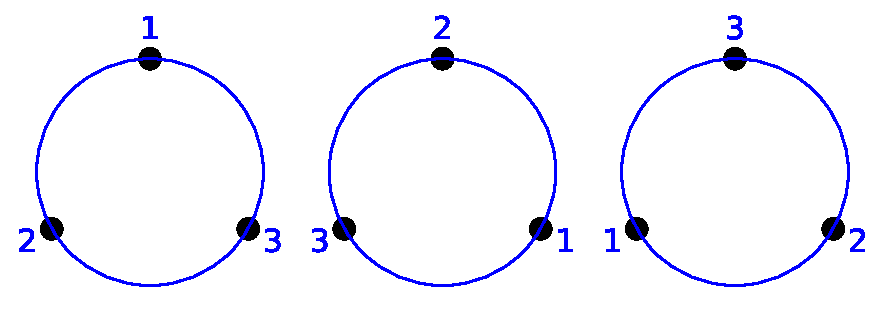
\includegraphics[width=\linewidth]{images/circequiv2}
\end{image}%
\tcblower
\end{figureptx}%
 Como não temos mais casos, o número total de permutações circulares com três elementos é 2.\end{proof}
\begin{theorem}{}{}{g:theorem:idp76}%
O número de permutações circulares com \(n\) elementos distintos é%
\begin{equation*}
PC_n = (n-1)! 
\end{equation*}
%
\end{theorem}
\begin{proof}{}{g:proof:idp77}
Se não considerássemos equivalentes disposições que possam coincidir por rotação, teríamos \(n!\) disposições.%
\par
Como para cada disposição, temos \(n\) disposições equivalentes, dividindo o total de permutações por \(n\), obtemos%
\begin{equation*}
PC(n) = \frac{n!}{n} = (n-1)! \qedhere
\end{equation*}
%
\end{proof}
\begin{technology}{}{g:technology:idp78}%
A lista com todas as permutações circulares, pode ser obtida com o seguinte comando: \leavevmode%
\begin{sageinput}
CyclicPermutations([1, 2, 3, 4]).list()
\end{sageinput}
\begin{sageoutput}
[[1, 2, 3, 4],
 [1, 2, 4, 3],
 [1, 3, 2, 4],
 [1, 3, 4, 2],
 [1, 4, 2, 3],
 [1, 4, 3, 2]]
\end{sageoutput}
%
\par
O número de permutações circulares com 10 elementos pode ser calculado da seguinte forma: \leavevmode%
\begin{sageinput}
PC(n) = factorial(n-1)
PC(10)
\end{sageinput}
\begin{sageoutput}
362880
\end{sageoutput}
%
\end{technology}
\begin{fact}{}{}{g:fact:idp79}%
Quantas rodas de ciranda podem ser formadas com 8 pessoas?%
\textbf{\blocktitlefont Solução}.\quad{}Basta calcular o número de permutações circulares de 8 elementos.%
\begin{equation*}
PC(8). 
\end{equation*}
\begin{sageinput}
PC(n) = factorial(n-1)
PC(8)
\end{sageinput}
\begin{sageoutput}
5040
\end{sageoutput}
\end{fact}
\begin{fact}{}{}{g:fact:idp80}%
Quantas rodas de ciranda podem ser formadas com 8 pessoas, se duas determinadas pessoas não podem ficar juntas?%
\textbf{\blocktitlefont Solução}.\quad{}Calculamos o número de permutações circulares com 8 elementos, \(PC(8)\). Agora, subtraimos desse total, o número de permutações de 8 elementos, na qual, dois deles estão juntos.%
\begin{figureptx}{Duas formas de organizar os elementos 1 e 2.}{x:figure:circequiv3}{}%
\begin{image}{0.1}{0.8}{0.1}%
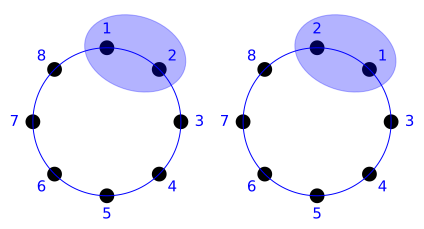
\includegraphics[width=\linewidth]{images/circ-equiv3}
\end{image}%
\tcblower
\end{figureptx}%
O que dá um total de \(PC(7)\times 2\) permutações circulares, pois temos duas formas de permutar os dois elementos que estão juntos, depois disso, olhamos para a roda de ciranda como se tivesse apenas 7 elementos. Portanto a resposta é%
\begin{equation*}
PC(8)-PC(7)\times2. 
\end{equation*}
%
\begin{sageinput}
PC(n) = factorial(n-1)
PC(8)-PC(7)*2
\end{sageinput}
\begin{sageoutput}
3600
\end{sageoutput}
\end{fact}
%
%
\typeout{************************************************}
\typeout{Exercícios 2.4.1 Exercícios}
\typeout{************************************************}
%
\begin{exercises-subsection}{Exercícios}{}{Exercícios}{}{}{g:exercises:idp81}
\begin{divisionexercise}{1}{}{}{g:exercise:idp82}%
De quantos modos 7 meninos e 7 meninas podem formar uma roda de ciranda de modo que pessoas de mesmo sexo não fiquem juntas?%
\par\smallskip%
\noindent\textbf{\blocktitlefont Resposta}.\hypertarget{g:answer:idp83}{}\quad{}3628800%
\end{divisionexercise}%
\begin{divisionexercise}{2}{}{}{g:exercise:idp84}%
De quantos modos 18 casais podem formar uma roda de ciranda de modo que cada homem permaneça ao lado de sua mulher?%
\par\smallskip%
\noindent\textbf{\blocktitlefont Resposta}.\hypertarget{g:answer:idp85}{}\quad{}93241325150797824000%
\end{divisionexercise}%
\end{exercises-subsection}
\end{sectionptx}
%
%
\typeout{************************************************}
\typeout{Seção 2.5 Permutações com Repetições}
\typeout{************************************************}
%
\begin{sectionptx}{Permutações com Repetições}{}{Permutações com Repetições}{}{}{x:section:section-permutacoes-com-repeticoes}
\begin{objectives}{Objetivos}{x:objectives:objetivos-permutacoes-repeticao}
%
\begin{enumerate}
\item{}Definir Permutação com Repetição.%
\item{}Mostrar como obter a lista com todas as permutações com repetições de \(n\) elementos no Sage.%
\item{}Mostrar como calcular o número de permutações com repetições de \(n\) elementos.%
\item{}Exemplificar.%
\end{enumerate}
\end{objectives}
\begin{fact}{}{}{g:fact:idp86}%
Quantos são os anagramas da palavra SAGEMATH?%
\textbf{\blocktitlefont Solução}.\quad{}Observe que a palavra SAGEMATH possui 8 letras, mas a letra A aparece duas vezes, o restante aparece apenas uma vez. Podemos imaginar, por enquanto, que a palavra é assim%
\begin{equation*}
SA_1GEMA_2TH
\end{equation*}
com \(A_1\neq A_2\), nesse caso teríamos um total de%
\begin{equation*}
P(8) = 8! 
\end{equation*}
permutações.%
\par
Agora vamos resolver o problema das repetições. Observe que para cada permutação, trocar os A's de lugar não muda o anagrama, portanto, precisamos dividir do total de permutações a quantidade de reordenar os A's. Dessa forma a resposta é%
\begin{equation*}
\frac{P(8)}{P(2)}=20160.
\end{equation*}
%
\end{fact}
\begin{definition}{}{g:definition:idp87}%
Quando permutamos uma lista de objetos, na qual, nem todos os elementos são distintos, precisamos considerar que permutar dois elementos idênticos não gera uma nova permutação. Este tipo de permutação é chamado de \emph{permutação com repetição}.%
\end{definition}
\begin{technology}{}{g:technology:idp88}%
Obtendo a lista com todas as permutações com repetições dos elementos \(1, 1, 1, 2, 2\): \begin{sageinput}
Permutations([1, 1, 1, 2, 2]).list()
\end{sageinput}
\begin{sageoutput}
[[1, 1, 1, 2, 2],
 [1, 1, 2, 1, 2],
 [1, 1, 2, 2, 1],
 [1, 2, 1, 1, 2],
 [1, 2, 1, 2, 1],
 [1, 2, 2, 1, 1],
 [2, 1, 1, 1, 2],
 [2, 1, 1, 2, 1],
 [2, 1, 2, 1, 1],
 [2, 2, 1, 1, 1]]
\end{sageoutput}
\end{technology}
\begin{definition}{}{g:definition:idp89}%
O número de permutações de \(n\) objetos, com um objeto repetido \(r_1\) vezes, outro objeto repetido \(r_2\) vezes, até o "último" objeto repetido \(r_k\) vezes, com%
\begin{equation*}
r_1+r_2+\cdots+r_k=n
\end{equation*}
é denotado por:%
\begin{equation*}
PR_n^{r_1, r_2, \ldots, r_k}. 
\end{equation*}
\end{definition}
\begin{theorem}{}{}{g:theorem:idp90}%
%
\begin{equation*}
PR_n^{r_1, r_2, \ldots, r_k} = \frac{n!}{r_1!\times r_2!\times\cdots\times r_k!}. 
\end{equation*}
%
\end{theorem}
\begin{proof}{}{g:proof:idp91}
Considere os \(n\) objetos da seguinte forma:%
\begin{equation*}
\underbrace{A_1A_1\ldots A_1}_{r_1  \text{ vezes}} \underbrace{A_2A_2\ldots A_2}_{r_2  \text{ vezes}}\ldots\underbrace{A_kA_k\ldots A_k}_{r_k  \text{ vezes}} 
\end{equation*}
observe que \(r_1+r_2+\cdots+ r_k = n.\) Para encontrar o número de formas de permutar esses elementos, vamos quebrar em \(k\) etapas. Na primeira etapa, vamos escolher \(r_1\) posições, dentre \(n\), para colocar \(A_1: C_n^{r_1}\). Na segunda etapa, vamos escolher \(r_2\) posições, dentre \(n-r_1\), para colocar \(A_2: C_{n-r_1}^{r_2}\). \(\ldots\) Na \(k\)-ésima etapa, vamos escolher \(r_k\) posições, dentre \(n-r_1-r_2-\cdots-r_{k-1}=r_k\), para colocar \(A_k: C_{r_k}^{r_k}\). Portanto,%
\begin{equation*}
PR_n^{r_1, r_2, \ldots, r_k} =~ C_n^{r_1}\times C_{n-r_1}^{r_2} \times \cdots \times C_{r_k}^{r_k} \\
\end{equation*}
Calculando cada \(C_x^y\)%
\begin{equation*}
PR_n^{r_1, r_2, \ldots, r_k} = \frac{n!}{r_1!\underbrace{(n-r_1)!}_{x_1}}\cdot\frac{\overbrace{(n-r_1)!}^{x_1}}{r_2!\underbrace{(n-r_1-r_2)!}_{x_2}}\cdots\frac{\overbrace{n_k!}^{x_k}}{n_k!\underbrace{(n_k-n_k)!}_{=1}}
\end{equation*}
E cancelando os \(x_i's\), obtemos%
\begin{equation*}
PR_n^{r_1, r_2, \ldots, r_k}= \frac{n!}{r_1!\times r_2!\times\cdots\times r_k!}.\qedhere
\end{equation*}
\end{proof}
\begin{technology}{}{g:technology:idp92}%
Obtendo o número de permutações com repetições no Sage, para \(n=10, r_1 = 3, r_2=2, r_3=2, r_4=1, r_5=1\) e \(r_6=1\): \begin{sageinput}
def PR(*lista):
    p = factorial(lista[0])
    for i in lista[1:]:
        p = p/factorial(i)
    return p
PR(10, 3, 2, 2)
\end{sageinput}
\begin{sageoutput}
151200
\end{sageoutput}
\end{technology}
\begin{fact}{}{}{g:fact:idp93}%
Quantos são os anagramas da palavra MATEMATICA?%
\textbf{\blocktitlefont Solução}.\quad{}Temos uma palavra com 10 letras. Das 10 letras, temos 3 A's, 2 M's e 2 T's e as outras aparecem uma única vez, portanto o número de anagramas desta palavra é%
\begin{equation*}
PR_{10}^{3, 2, 2} = 151200. 
\end{equation*}
%
\end{fact}
\begin{fact}{}{}{g:fact:idp94}%
Quantos são os anagramas da palavra MATEMATICA que começam por vogal?%
\textbf{\blocktitlefont Solução}.\quad{}Se o anagrama começa por vogal, temos as possibilidades, A ou E ou I.%
\par
Começando com A, temos um total de \(PR_9^{2, 2, 2}\), começando com E, temos um total de \(PR_9^{3, 2, 2}\) e começando com I, temos um total de \(PR_9^{3, 2, 2}\) Portanto a resposta é%
\begin{equation*}
PR_9^{2, 2, 2} + 2\times PR_9^{3, 2, 2} = 75600. 
\end{equation*}
%
\end{fact}
%
%
\typeout{************************************************}
\typeout{Exercícios 2.5.1 Exercícios}
\typeout{************************************************}
%
\begin{exercises-subsection}{Exercícios}{}{Exercícios}{}{}{g:exercises:idp95}
\begin{divisionexercise}{1}{}{}{g:exercise:idp96}%
\terminology{(OPEMAT - 2016 - nível 2)} A figura abaixo representa o mapa de uma cidade. Cada aresta representa uma rua e cada vértice representa um cruzamento. Quantos são os trajetos de comprimento mínimo ligando o ponto A ao ponto B?%
\begin{figureptx}{Mapa da cidade.}{x:figure:mapa}{}%
\begin{image}{0.275}{0.45}{0.275}%
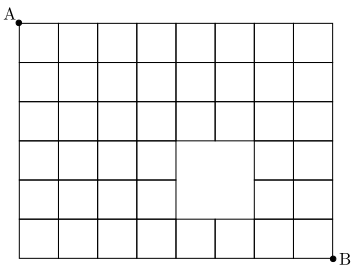
\includegraphics[width=\linewidth]{images/permut}
\end{image}%
\tcblower
\end{figureptx}%
\par\smallskip%
\noindent\textbf{\blocktitlefont Resposta}.\hypertarget{g:answer:idp97}{}\quad{}1743%
\end{divisionexercise}%
\begin{divisionexercise}{2}{}{}{g:exercise:idp98}%
Quantos números de 8 dígitos, maiores que 50.000.000, podem ser formados usando apenas os algarismos 1, 2, 5, 5, 5, 7, 7, 7?%
\par\smallskip%
\noindent\textbf{\blocktitlefont Resposta}.\hypertarget{g:answer:idp99}{}\quad{}840%
\end{divisionexercise}%
\begin{divisionexercise}{3}{}{}{g:exercise:idp100}%
De quantos modos podemos colocar em fila 6 letras A, 6 letras B, 5 letras C e 4 letras D, de modo que não haja duas letras C juntas?%
\par\smallskip%
\noindent\textbf{\blocktitlefont Resposta}.\hypertarget{g:answer:idp101}{}\quad{}10406235840%
\end{divisionexercise}%
\begin{divisionexercise}{4}{}{}{g:exercise:idp102}%
De quantos modos podem ser pintados 15 objetos iguais usando 6 cores diferentes?%
\par\smallskip%
\noindent\textbf{\blocktitlefont Resposta}.\hypertarget{g:answer:idp103}{}\quad{}15504%
\end{divisionexercise}%
\begin{divisionexercise}{5}{}{}{g:exercise:idp104}%
Quantas são as opções que temos de colocar 10 bolinhas \((\bullet)\) e 7 barras \((~|~)\) em sequência?%
\par\smallskip%
\noindent\textbf{\blocktitlefont Resposta}.\hypertarget{g:answer:idp105}{}\quad{}19448%
\end{divisionexercise}%
\end{exercises-subsection}
\end{sectionptx}
%
%
\typeout{************************************************}
\typeout{Seção 2.6 Combinações Completas}
\typeout{************************************************}
%
\begin{sectionptx}{Combinações Completas}{}{Combinações Completas}{}{}{x:section:section-combinacoes-completas}
\begin{objectives}{Objetivos}{x:objectives:objetivos-combinacoes-completas}
%
\begin{enumerate}
\item{}Definir combinação completa.%
\item{}Mostrar como obter a lista com todas as permutações com repetições de \(n\) elementos.%
\item{}Mostrar como calcular o número de permutações com repetições de \(n\) elementos.%
\item{}Exemplificar.%
\end{enumerate}
\end{objectives}
Vamos começar com um exemplo que ilustra bem a noção de \emph{Combinação Completa}.%
\begin{fact}{}{}{x:fact:exem-com-completa}%
De quantos modos é possível comprar 3 sorvetes em uma loja que oferece 6 sabores? Obs. Supondo que de cada sabor estejam disponíveis pelo menos 3 unidades.%
\textbf{\blocktitlefont Solução}.\quad{}Resolver este problema é o mesmo que encontrar o número de soluções da equação:%
\begin{equation}
x_1 + x_2 + x_3 + x_4 + x_5 + x_6  = 3, ~~~ \text{ com }  x_i \geq 0 \label{x:men:eq-comb-completa}
\end{equation}
na qual, cada \(x_i, i\in\{1, 2, 3, 4, 5, 6\}\) representa a quantidade de sorvetes do sabor \(i\). Claramente, temos a restrição \(x_i\geq 0\), pois não podemos pegar uma quantidade negativa de sorvetes.%
\par
A equação \hyperref[x:men:eq-comb-completa]{({\xreffont\ref{x:men:eq-comb-completa}})} pode ser interpretada de tal forma que, encontrar o número de soluções será o mesmo que calcular o número de permutações com repetições de uma sequência de dois tipos de elementos. Vamos explicar esta interpretação:%
\par
Coloque um traço separando uma incógnita da outra. Para representar a quantidade de sorvetes de um tipo \(i\), coloque a quantidade de bolas entre os traços que representam o sabor \(i\). Assim a solução%
\begin{equation*}
x_1=1, ~ x_5=2, ~ x_i=0, ~~ i\in \{2, 3, 4, 6\} 
\end{equation*}
é representada por:%
\begin{figureptx}{Representação de uma das soluções.}{x:figure:combinacao-completa}{}%
\begin{image}{0.3}{0.4}{0.3}%
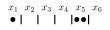
\includegraphics[width=\linewidth]{images/combinacaocompleta}
\end{image}%
\tcblower
\end{figureptx}%
Observe que cada permutação dessa representação de traços e bolas é uma solução da Equação \hyperref[x:men:eq-comb-completa]{({\xreffont\ref{x:men:eq-comb-completa}})} e que cada solução da Equação \hyperref[x:men:eq-comb-completa]{({\xreffont\ref{x:men:eq-comb-completa}})} pode ser representada com traços de bolas (Existe uma bijeção entre as duas coisas).%
\par
Portanto para encontrar o número de soluções da Equação \hyperref[x:men:eq-comb-completa]{({\xreffont\ref{x:men:eq-comb-completa}})}, basta calcular%
\begin{equation*}
PR_8^{5, 3} = 56 
\end{equation*}
Pois, temos 5 traços e 3 bolas, então estamos permutando um total de 8 elementos, sendo 5 de um tipo e 3 de outro tipo.%
\end{fact}
\begin{definition}{}{g:definition:idp106}%
O número de \emph{combinações completas} de \(n\) elementos, tomados \(p\) a \(p\) é o número de formas de escolher \(p\) elementos dentre \(n\) disponíveis, podendo escolher repetidamente os objetos, até obter a quantidade \(p\).%
\par
O número de combinações completas de \(n\) elementos, tomados \(p\) a \(p\) é denotado por:%
\begin{equation*}
CR_n^{p} 
\end{equation*}
%
\end{definition}
\begin{remark}{}{g:remark:idp107}%
As combinações completas dos objetos \(1, 2, 3, 4\) tomados 3 a 3 são: \begin{sageinput}
Combinations([1, 1, 1, 2, 2, 2, 3, 3, 3, 4, 4, 4], 3).list()
\end{sageinput}
\begin{sageoutput}
[[1, 1, 1],
 [1, 1, 2],
 [1, 1, 3],
 [1, 1, 4],
 [1, 2, 2],
 [1, 2, 3],
 [1, 2, 4],
 [1, 3, 3],
 [1, 3, 4],
 [1, 4, 4],
 [2, 2, 2],
 [2, 2, 3],
 [2, 2, 4],
 [2, 3, 3],
 [2, 3, 4],
 [2, 4, 4],
 [3, 3, 3],
 [3, 3, 4],
 [3, 4, 4],
 [4, 4, 4]]
\end{sageoutput}
\end{remark}
\begin{theorem}{}{}{g:theorem:idp108}%
%
\begin{equation*}
CR_n^p = PR_{p+n-1}^{p, n-1} = C_{p+n-1}^p
\end{equation*}
%
\end{theorem}
\begin{proof}{}{g:proof:idp109}
Calcular \(CR_n^p\) é o mesmo que encontrar o número de soluções da equação:%
\begin{equation*}
x_1 + x_2 + x_3 + \ldots + x_n  = p, ~~~ \text{ com }  x_i \geq 0 
\end{equation*}
Usando a ideia da representação de "bolas e traços" da Solução do (\hyperref[x:fact:exem-com-completa]{Exemplo~{\xreffont\ref{x:fact:exem-com-completa}}}) vamos ficar com \(p\) bolas e \(n-1\) traços. O cálculo do número de permutações destes \(p+n-1\) objetos com \(p\) objetos de um tipo e \(n-1\) objetos de outro tipo é dado por:%
\begin{equation*}
PR_{p+n-1}^{p, n-1} = C_{p+n-1}^p \qedhere
\end{equation*}
\end{proof}
\begin{technology}{}{g:technology:idp110}%
Para obter o número de combinações completas de \(n\),tomados \(p\) a \(p\), usamos o código binomial(p+n-1, p).%
\begin{sageinput}
CR(n, p) = binomial(p+n-1, p)
CR(6, 3)
\end{sageinput}
\begin{sageoutput}
56
\end{sageoutput}
\end{technology}
\begin{fact}{}{}{g:fact:idp111}%
Quantas são as soluções inteiras e não negativas de%
\begin{equation*}
x_1 + x_2 + x_3 + \ldots + x_{10}  = 20?
\end{equation*}
%
\textbf{\blocktitlefont Solução}.\quad{}O número de soluções desta equação, com \(x_i\in \mathbb{Z} \text{ e } x_i\geq 0, i\in\{1, 2, \ldots, 10\}\)  é o  número de combinações completas de 10 elementos, tomandos 20 a 20:%
\begin{equation*}
CR_{10}^{20}
\end{equation*}
%
\begin{sageinput}
CR(n, p) = binomial(p+n-1, p) 
CR(10, 20)
\end{sageinput}
\begin{sageoutput}
10015005
\end{sageoutput}
\end{fact}
\begin{fact}{}{}{g:fact:idp112}%
Quantas são as soluções inteiras da equação%
\begin{equation*}
x_1 + x_2 + x_3 = 15
\end{equation*}
com \(x_1>0\), \(x_2\geq 2\) e \(x_3 \geq 4\)?%
\textbf{\blocktitlefont Solução}.\quad{}Defina%
\begin{equation*}
x_1 = x+1, 
\end{equation*}
%
\begin{equation*}
x_2 = y+2 
\end{equation*}
%
\begin{equation*}
x_3 = z+4 
\end{equation*}
Substituindo, temos%
\begin{equation*}
(x+1) + (y+2) + (z+4) = 15 
\end{equation*}
ou seja%
\begin{equation*}
x + y + z = 8 ~~~~ (\clubsuit) 
\end{equation*}
Desta forma, o número de soluções de \((\clubsuit)\) será a solução do problema, pois, quando \(x=0\) teremos \(x_1=1\), quando \(y=0\) teremos \(x_2=2\) e quando \(z=0\) teremos \(x_3=4\). Portanto a resposta é%
\begin{equation*}
CR_3^{8} = 45. 
\end{equation*}
%
\end{fact}
\begin{fact}{}{}{g:fact:idp113}%
Quantas são as soluções inteiras e não negativas de%
\begin{equation}
x_1 + x_2 + x_3 + x_4  \leq 50?\label{x:men:sol-desi}
\end{equation}
%
\textbf{\blocktitlefont Solução}.\quad{}Observe que uma possibilidade seria calcular o número de soluções de cada um dos casos:%
\begin{equation}
\begin{cases} x_1 + x_2 + x_3 + x_4  = 0,\\
x_1 + x_2 + x_3 + x_4  = 1\\
\vdots \\
x_1 + x_2 + x_3 + x_4  = 50.\end{cases}\label{x:men:sol-igual}
\end{equation}
A soma do número de soluções de cada um dos casos é a resposta, no entanto, é inviável fazer tal cálculo. Felizmente temos outra forma de resolver este problema.%
\par
Observe que existe uma bijeção entre o conjunto das soluções de \hyperref[x:men:sol-desi]{({\xreffont\ref{x:men:sol-desi}})} com o conjunto das soluções da equação \hyperref[x:men:sol-desi2]{({\xreffont\ref{x:men:sol-desi2}})}:%
%
\begin{equation}
x_1 + x_2 + x_3 + x_4 + y  = 50.\label{x:men:sol-desi2}
\end{equation}
Para entender a bijeção, observe o seguinte. Somando \(50-i, i\in \{0, 1, 2, \ldots, 50\}\), nos dois lados da igualdade, na linha \(i, i\in \{0, 1, 2, \ldots, 50\}\) de \hyperref[x:men:sol-igual]{({\xreffont\ref{x:men:sol-igual}})}, não mudamos absolutamente nada e ficamos com:%
%
\begin{equation}
\begin{cases} x_1 + x_2 + x_3 + x_4 + 50 = 0 + 50,\\
x_1 + x_2 + x_3 + x_4 + 49  = 1 +49 \\
\vdots \\
x_1 + x_2 + x_3 + x_4 + 0  = 50+0.\end{cases}\label{g:men:idp114}
\end{equation}
Cada solução da linha \(i\), é uma solução de \hyperref[x:men:sol-desi2]{({\xreffont\ref{x:men:sol-desi2}})} com o valor de \(y\) igual a \(50-i\). E para cada \(y\in \{0, 1, 2, \ldots, 50\}\) a solução de \hyperref[x:men:sol-desi2]{({\xreffont\ref{x:men:sol-desi2}})} vai ser a solução da linha \(y\) de \hyperref[x:men:sol-igual]{({\xreffont\ref{x:men:sol-igual}})} .%
\par
Portanto a resposta é o número de solução da equação \hyperref[x:men:sol-desi2]{({\xreffont\ref{x:men:sol-desi2}})} que é dado por:%
%
\begin{equation*}
CR_5^{50} = 316251. 
\end{equation*}
\end{fact}
\begin{fact}{}{}{g:fact:idp115}%
\terminology{(VESTIBULAR UFPE – UFRPE \slash{} 1998 2ª ETAPA)}Semelhante ao dominó, mas feito de pedras triangulares equiláteras, o jogo de trominó apresenta na face triangular superior um certo número de pontos com repetições, escolhidos de 1 a n, dispostos ao longo de cada aresta (ver figura).%
\begin{figureptx}{Uma das peças com os valores 1, 2 e 4.}{x:figure:tro}{}%
\begin{image}{0.375}{0.25}{0.375}%
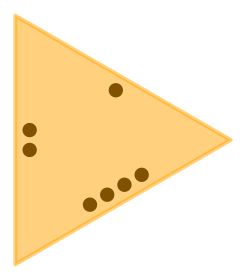
\includegraphics[width=\linewidth]{images/tro}
\end{image}%
\tcblower
\end{figureptx}%
Quantas peças há no trominó, supondo n = 6?%
\textbf{\blocktitlefont Solução}.\quad{}Observe que os números estão em disposição circular, então vamos separar as peças em três tipos:%
%
\begin{enumerate}
\item{}Todos os lados com o mesmo valor. Cada peça pode ser formada de uma única forma.%
\item{}Dois lados possuem um valor e o terceiro lado possui um valor diferente. Cada peça pode ser formada de uma única forma, pois o número de permutações circulares com 3 elementos é 2, mas como temos duas entradas iguais, precisamos dividir por 2.%
\item{}Cada lado possui um valor diferente. Cada peça pode ser formada de duas formas, pois o número de permutações circulares com 3 elementos é 2.%
\end{enumerate}
Inicialmente, vamos contar como se em cada tipo, as peças só pudessem ser formadas de uma forma, depois vamos acrescentar a quantidade de peças do terceiro tipo, que fica faltando nessa contagem inicial.%
\par
Temos que escolher os valores de cada um dos 3 lados de cada peça do trominó. Como os valores vão de 1 até 6 e são 3 lados, o número de peças do trominó (sem contar as permutações circulares) para \(n=6\) é o número de soluções inteiras não negativas da equação:%
\begin{equation*}
x_1 + x_2 + x_3 + x_4 + x_ 5 + x_ 6 = 3, 
\end{equation*}
que é dado por \(CR_6^3\).%
\par
Agora precisamos contar as peças, do terceiro tipo, que estão faltando. Como os três valores são diferentes, temos 6 opções de valores para escolher 3 e para cada escolha, temos duas formas de organizar na peça do trominó, portanto o número de peças desse tipo é:%
\begin{equation*}
2\times C_6^3 =40. 
\end{equation*}
Já que, a metade das peças do terceiro tipo foram contadas uma vez pela combinação completa, \(CR_6^3\), a quantidade total de peças é:%
\begin{equation*}
CR_6^{3} + C_6^3 = 56+20 = 76. 
\end{equation*}
%
\end{fact}
%
%
\typeout{************************************************}
\typeout{Exercícios 2.6.1 Exercícios}
\typeout{************************************************}
%
\begin{exercises-subsection}{Exercícios}{}{Exercícios}{}{}{g:exercises:idp116}
\begin{divisionexercise}{1}{}{}{g:exercise:idp117}%
Quantas são as soluções inteiras positivas de \(x+y+z+w = 15\)?%
\par\smallskip%
\noindent\textbf{\blocktitlefont Resposta}.\hypertarget{g:answer:idp118}{}\quad{}816%
\end{divisionexercise}%
\begin{divisionexercise}{2}{}{}{g:exercise:idp119}%
Quantas são as peças de um dominó comum?%
\par\smallskip%
\noindent\textbf{\blocktitlefont Resposta}.\hypertarget{g:answer:idp120}{}\quad{}28%
\end{divisionexercise}%
\begin{divisionexercise}{3}{}{}{g:exercise:idp121}%
Quantas são as soluções inteiras não-negativas de \(x_1+x_2+x_3+x_4+x_5 = 8\) nas quais \(x_1>x_2\)?%
\par\smallskip%
\noindent\textbf{\blocktitlefont Resposta}.\hypertarget{g:answer:idp122}{}\quad{}200%
\end{divisionexercise}%
\begin{divisionexercise}{4}{}{}{g:exercise:idp123}%
Quantos inteiros entre \(1\) e \(100.000.000\), inclusive, possui a propriedade: "cada dígito é menor ou igual ao seu sucessor"?%
\par\smallskip%
\noindent\textbf{\blocktitlefont Resposta}.\hypertarget{g:answer:idp124}{}\quad{}24309%
\end{divisionexercise}%
\begin{divisionexercise}{5}{}{}{g:exercise:idp125}%
De quantas maneiras é possível colocar 10 anéis diferentes em 8 dedos?%
\par\smallskip%
\noindent\textbf{\blocktitlefont Resposta}.\hypertarget{g:answer:idp126}{}\quad{}70572902400%
\end{divisionexercise}%
\end{exercises-subsection}
\end{sectionptx}
\end{chapterptx}
%
%
\typeout{************************************************}
\typeout{Capítulo 3 Outros Métodos de Contagem}
\typeout{************************************************}
%
\begin{chapterptx}{Outros Métodos de Contagem}{}{Outros Métodos de Contagem}{}{}{x:chapter:contagem2}
\begin{introduction}{}%
As Seções: Princípio da Inclusão-Exclusão, Permutações Caóticas e Os Lemas de Kaplansky, foram elaborados a partir da dissertação do ProfMat \hyperlink{x:biblio:luiz}{[{\xreffont 6.9}]}. Nas duas últimas destas três Seções, estão disponíveis formas interativas de gerar o número de soluções e as soluções explicitamente.%
\par
A Seção sobre o Princípio da Casa dos Pombos, foi feita com o conteúdo do artigo \hyperlink{x:biblio:oxente01}{[{\xreffont 6.8}]} do jornal \href{http://ematematicaoxente.com.br/}{\terminology{É matemática, oxente!}}.%
\end{introduction}%
%
%
\typeout{************************************************}
\typeout{Seção 3.1 Princípio da Inclusão-Exclusão}
\typeout{************************************************}
%
\begin{sectionptx}{Princípio da Inclusão-Exclusão}{}{Princípio da Inclusão-Exclusão}{}{}{x:section:section-inclusao-exclusao}
\begin{objectives}{Objetivos}{x:objectives:objetivos-aditivo-multiplicativo}
%
\begin{enumerate}
\item{}Enunciar e demonstrar o Princípio da Inclusão-Exclusão, para 2, 3 e \(n\) conjuntos.%
\item{}Exemplificar.%
\item{}Resolver um exemplo no Sage.%
\end{enumerate}
\end{objectives}
%
%
\typeout{************************************************}
\typeout{Subseção 3.1.1 O Princípio da Inclusão-Exclusão para 2 e 3 conjuntos}
\typeout{************************************************}
%
\begin{subsectionptx}{O Princípio da Inclusão-Exclusão para 2 e 3 conjuntos}{}{O Princípio da Inclusão-Exclusão para 2 e 3 conjuntos}{}{}{g:subsection:idp127}
\begin{theorem}{}{}{x:theorem:teo-inclusao-exclusao-2}%
Sejam  \(A\)  e  \(B\)  conjuntos finitos, então%
\begin{equation*}
\#(A\cup B) = \#A + \# B - \#(A\cap B). 
\end{equation*}
%
\begin{figureptx}{Diagrama de Venn para \((A\cup B)\).}{x:figure:inclusao-exclusao-2}{}%
\begin{image}{0.35}{0.3}{0.35}%
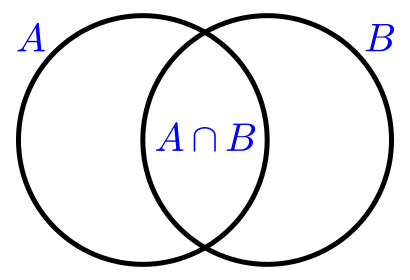
\includegraphics[width=\linewidth]{images/inclusaoexclusao2}
\end{image}%
\tcblower
\end{figureptx}%
Ou seja, a cardinalidade de \(A\cup B\) é igual a cardinalidade de \(A\) mais a cardinalidade de \(B\) menos a cardinalidade de \(A\cap B\).%
\end{theorem}
\begin{proof}{}{g:proof:idp128}
Sejam \(A\) e \(B\) conjuntos finitos, \(T_1\) a tarefa de selecionar um elemento de \(A\) e \(T_2\) a tarefa de selecionar um elemento de \(B\).%
\par
Existem \(\#A\) maneiras de realizar \(T_1\) e \(\#B\) maneiras de realizar \(T_2\). O número de maneiras de executar \(T_1\) ou \(T_2\) é a soma do número de maneiras de executar \(T_1\) com o número de maneiras de executar \(T_2\) menos o número  de maneiras de  executar ambos \(T_1\) e \(T_2\), pois esta quantidade já foi contada duas vezes.%
\par
Como existem \(\#(A\cup B)\) maneiras de realizar \(T_1\) ou \(T_2\) e \(\#(A\cap B)\) maneiras de realizar \(T_1\) e \(T_2\), temos:%
\begin{equation*}
\#(A\cup B)=\#A+\#B-\#(A\cap B).\qedhere
\end{equation*}
%
\end{proof}
\begin{fact}{}{}{g:fact:idp129}%
Numa pesquisa com jovens foram feitas as seguintes perguntas para que respondessem sim ou não. Gosta de exatas? Gosta de humanas? Responderam sim a primeira pergunta 80 jovens, 60 reponderam sim a segunda e 15 responderam sim a ambas. Quantos jovens foram entrevistados?%
\textbf{\blocktitlefont Solução}.\quad{}Defina \(E\) como o conjunto dos alunos entrevistados que gostam de exatas e defina \(H\) como o conjunto dos alunos entrevistados que gostam de humanas, assim%
\begin{equation*}
\#E=80, \#H = 60 \text{ e }\#(E\cap H) = 15.
\end{equation*}
Dessa forma, calculando \(\#E+\#H\) o número de alunos que gostam de ambas as áreas é contado duas vezes. Portanto, para determinar o número de alunos entrevistados, retira-se o número de alunos que foi contado duas vezes, ou seja%
\begin{equation*}
\#(E\cup H)= \#E+\#H-\#(E\cap H) = 80 + 60-15 = 125.
\end{equation*}
%
\end{fact}
\begin{theorem}{}{}{g:theorem:idp130}%
Sejam  \(A, B\) e  \(C\)  conjuntos finitos, então%
%
\begin{align*}
\#(A\cup B\cup C) = \amp ~\#(A)+\#(B)+\#(C) \\
\amp ~ -\#(A\cap B)-\#(A\cap C)-\#(B\cap C) \\
\amp ~ +\#(A\cap B\cap C). 
\end{align*}
\begin{figureptx}{Diagrama de Venn para \((A\cup B\cup C)\).}{x:figure:inclusao-exclusao-3}{}%
\begin{image}{0.15}{0.7}{0.15}%
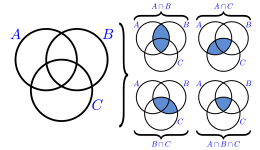
\includegraphics[width=\linewidth]{images/inclusaoexclusao3novo}
\end{image}%
\tcblower
\end{figureptx}%
\end{theorem}
\begin{proof}{}{g:proof:idp131}
Considere \((A\cup B)\) como um conjunto, usando o (\hyperref[x:theorem:teo-inclusao-exclusao-2]{Teorema~{\xreffont\ref{x:theorem:teo-inclusao-exclusao-2}}}) temos:%
\begin{align*}
\#[A\cup B\cup C] = \amp~\#[(A\cup B)\cup C] \\
= \amp ~\#(A\cup B)+\#C-\#[(A\cup B)\cap C] \\
= \amp ~ \#A+\#B-\#(A\cap B)+\#C-\#[(A\cup B)\cap C]. 
\end{align*}
Usando a igualdade:%
\begin{equation*}
(A\cup B)\cap C = (A\cap C)\cup (B\cap C), 
\end{equation*}
temos%
\begin{equation*}
\#[A\cup B\cup C] = \#A+\#B-\#(A\cap B)+\#C-\#[(A\cap C)\cup (B\cap C)]. 
\end{equation*}
Aplicando o (\hyperref[x:theorem:teo-inclusao-exclusao-2]{Teorema~{\xreffont\ref{x:theorem:teo-inclusao-exclusao-2}}}) na união \([(A\cap C)\cup (B\cap C)]\), concluímos a demonstração:%
\begin{align*}
\#(A\cup B\cup C) = \amp ~\#A+\#B-\#(A\cap B)+\#C \\
\amp ~ -\#(A\cap C)-\#(B\cap C) \\
\amp ~ +\#(A\cap B\cap C). \qedhere
\end{align*}
%
\end{proof}
\end{subsectionptx}
%
%
\typeout{************************************************}
\typeout{Subseção 3.1.2 O Princípio da Inclusão-Exclusão para \(n\) conjuntos}
\typeout{************************************************}
%
\begin{subsectionptx}{O Princípio da Inclusão-Exclusão para \(n\) conjuntos}{}{O Princípio da Inclusão-Exclusão para \(n\) conjuntos}{}{}{g:subsection:idp132}
\begin{theorem}{}{}{x:theorem:teo-inclusao-exclusao-n}%
Sejam \(A_1,A_2,\cdots,A_n\) conjuntos finitos. A cardinalidade de%
\begin{equation*}
\bigcup_{i=1}^{n}A_i =  A_1 \cup A_2 \cup \cdots \cup A_n ~~~~ (\blacklozenge)
\end{equation*}
é dada por:%
\begin{equation*}
(\bigstar)  \begin{cases} \displaystyle\#\bigcup_{i=1}^{n}A_i \amp \displaystyle=  \sum_{i=1}^{n}\#A_i-\sum_{0 \lt  i \lt j   \leq n}\#(A_i\cap A_j)+\cdots\\
\amp ~~~~~ \displaystyle\cdots  +(-1)^{n-1}\#(A_1\cap A_2\cap \cdots\cap A_n) \end{cases}
\end{equation*}
%
\end{theorem}
\begin{proof}{}{g:proof:idp133}
Vamos verificar que a fórmula é verdadeira mostrando que um elemento da união \((\blacklozenge)\) é contada exatamente uma vez pelo lado direito da Expressão \((\bigstar)\).%
\par
Suponha que o elemento \(a\) pertence a exatamente \(r\) (\(1\leq r\leq n\)) dos conjuntos \(A_1, A_2, \ldots, A_n\).%
\par
O elemento \(a\) é contado \(C_r^1\) vezes por \(\sum_{i=1}^{n}\#A_i, C_r^2\) vezes por \(\sum_{0\lt i \lt j\leq n}\#(A_i\cap A_j)\), e de forma geral \(C_r^m\) vezes, pelo somatório envolvendo \(m\) dos conjuntos \(A_i\). Assim, este elemento será contado exatamente%
\begin{equation*}
C_r^1-C_r^2+C_r^3-\cdots+(-1)^{r+1}C_r^r
\end{equation*}
vezes pelo lado direito de \((\bigstar)\). Usando a Expansão do Binômio de Newton, temos%
\begin{equation*}
0 = (1-1)^p = C_r^0 -(C_r^1-C_r^2+C_r^3-\cdots+(-1)^{r+1}C_r^r). 
\end{equation*}
Portanto%
\begin{equation*}
C_r^1-C_r^2+C_r^3-\cdots+(-1)^{r+1}C_r^r = C_r^0 = 1. 
\end{equation*}
Isto mostra que o elemento \(a\) é contado exatamente uma vez pelo lado direito de \((\bigstar)\).%
\end{proof}
\begin{fact}{}{}{g:fact:idp134}%
Quantos são os anagramas da palavra COMPLEXA que tem C em 1º lugar, ou O em 2º lugar, ou M em 3º lugar ou P em 4º lugar?%
\textbf{\blocktitlefont Solução}.\quad{}Sejam%
\begin{equation*}
\bullet A_1 \text{o conjunto dos anagramas de COMPLEXA que tem C em 1º lugar}
\end{equation*}
%
\begin{equation*}
\bullet A_2 \text{o conjunto dos anagramas de COMPLEXA que tem O em 2º lugar}
\end{equation*}
%
\begin{equation*}
\bullet A_3 \text{o conjunto dos anagramas de COMPLEXA que tem M em 3º lugar}
\end{equation*}
%
\begin{equation*}
\bullet A_4 \text{o conjunto dos anagramas de COMPLEXA que tem P em 4º lugar}
\end{equation*}
Assim, \(\#A_i = 7!,\) para  \(i\in \{1, 2, 3, 4\}\).%
\par
Observe que \(\#(A_i\cap A_j), 1\leq i\lt j\leq 4\) é o número de anagramas da palavra COMPLEXA que estão em dois dos conjuntos \(A_i's, i\in\{1, 2, 3, 4\}\), logo%
\begin{equation*}
\#(A_i\cap A_j) = 6!
\end{equation*}
%
\par
Observe que \(\#(A_i\cap A_j\cap A_k), 1\leq i\lt j\leq 4\) é o número de anagramas da palavra COMPLEXA que estão em três dos conjuntos \(A_i's, i\in\{1, 2, 3, 4\}\), logo%
\begin{equation*}
\#(A_i\cap A_j\cap A_k) = 5!
\end{equation*}
%
\par
Observe que \(\#(A_1\cap A_2\cap A_3\cap A_4)\) é o número de anagramas da palavra COMPLEXA que tem as letras C, O, M e P  nas posições \(1, 2, 3, 4\) fixas, logo%
\begin{equation*}
\#(A_1\cap A_2\cap A_3\cap A_4) = 4!
\end{equation*}
Pelo Princípio da Inclusão-Exclusão (\hyperref[x:theorem:teo-inclusao-exclusao-n]{Teorema~{\xreffont\ref{x:theorem:teo-inclusao-exclusao-n}}}),%
\begin{align*}
\#(A_1\cup A_2\cup A_3\cup A_4) = \amp ~\sum_{i=1}^{4} \#A_i - \sum_{1\leq i\lt j\leq 4} \#(A_i\cap A_j) \\
\amp ~ +\sum_{1\leq i\lt j\lt k \leq 4} \#(A_i\cap A_j\cap A_k) \\
\amp ~ -\#(A_1\cap A_2\cap A_3\cap A_4). 
\end{align*}
Organizando, temos%
\begin{align*}
\#(A_1\cup A_2\cup A_3\cup A_4) = \amp ~ 4\times\#A_1 - C_4^2\times\#(A_1\cap A_2) \\
\amp ~ +C_4^3\times\#(A_1\cap A_2\cap A_3) \\
\amp ~ -\#(A_1\cap A_2\cap A_3\cap A_4). 
\end{align*}
Substituindo, temos%
\begin{align*}
\#(A_1\cup A_2\cup A_3\cup A_4) = \amp ~ 4\times 7! - C_4^2\times 6! +C_4^3\times 5! -4! \\
=\amp ~ 16296. 
\end{align*}
%
\end{fact}
\begin{fact}{}{}{g:fact:idp135}%
Qual é o número de elementos do conjunto: a)%
%
\begin{equation*}
A = \{ a\in \mathbb{N}~|~ a \text{ é múltiplo de } 2, 3 \text{ ou } 5 \text{ menor que } 10000\}; 
\end{equation*}
b)%
%
\begin{equation*}
B = \{ b\in \mathbb{N}~|~ b \text{ é múltiplo de } 2, 3, 5, 7, 11, 13, 17 \text{ ou } 19 \text{ menor que } 10000\}. 
\end{equation*}
%
\textbf{\blocktitlefont Solução 1}.\quad{}\terminology{item a)} Sejam%
\begin{equation*}
\bullet A_2=\{n\in\mathbb{N}~|~ 1\leq n\leq 10000 \text{ e } n \text{ é múltiplo de 2}\}
\end{equation*}
%
\begin{equation*}
\bullet A_3=\{n\in\mathbb{N}~|~ 1\leq n\leq 10000 \text{ e } n \text{ é múltiplo de 3}\}
\end{equation*}
%
\begin{equation*}
\bullet A_5=\{n\in\mathbb{N}~|~ 1\leq n\leq 10000 \text{ e } n \text{ é múltiplo de 5}\}
\end{equation*}
A resposta do item a) é a cardinalidade do conjunto:%
\begin{equation*}
A_2\cup A_3\cup A_5. 
\end{equation*}
Pelo Princípio da Inclusão-Exclusão (\hyperref[x:theorem:teo-inclusao-exclusao-n]{Teorema~{\xreffont\ref{x:theorem:teo-inclusao-exclusao-n}}}):%
\begin{align*}
\#(A_2\cup A_3\cup A_5) = \amp ~  \#A_2+\#A_3+\#A_5 \\
\amp ~ - \#(A_2\cap A_3) - \#(A_2\cap A_5) - \#(A_3\cap A_5) \\
\amp ~ +\#(A_2\cap A_3\cap A_5). 
\end{align*}
Para obter a cardinalidade de cada um dos conjuntos \(A_i's\), vamos dividir 10000 por \(i\), pois se obtermos \(10000 = p\times i + r\), na divisão Euclideana, significa que \(1\times i, 2\times i, \ldots, p\times i \) são todos múltiplos de \(i\) e são menores que 10000. Fazendo as divisões obtemos:%
\begin{align*}
10000 \amp =  ~ 5000\times 2 + 0 \Rightarrow \#A_2 = 5000 \\
10000 \amp =  ~ 3333\times 3 + 1 \Rightarrow \#A_3 = 3333 \\
10000 \amp =  ~ 2000\times 5 + 0 \Rightarrow \#A_5 = 2000. 
\end{align*}
Para obter a cardinalidade de cada uma das interseções \(A_i\cap A_j\), vamos dividir 10000 por \(i\times j\):%
\begin{align*}
10000 \amp =  ~ 1666\times 6 + 4 \Rightarrow \#(A_2\cap A_3) = 1666 \\
10000 \amp =  ~ 1000\times 10 + 0 \Rightarrow \#(A_2\cap A_5) = 1000 \\
10000 \amp =  ~ 666\times 15 + 10 \Rightarrow \#(A_3\cap A_5) = 666. 
\end{align*}
Para obter a cardinalidade de \(A_2\cap A_3\cap A_5\), vamos dividir 10000 por \(2\times 3\times 5\):%
\begin{align*}
10000 \amp =  ~ 333\times 30 + 10 \Rightarrow \#(A_2\cap A_3\cap A_5) = 333. 
\end{align*}
Portanto, pelo Princípio Inclusão-Exclusão temos:%
\begin{align*}
\#(A_2\cup A_3\cup A_5) \amp =  5000+3333+2000-1666-1000-666+333 \\
\amp =  ~ 7334 
\end{align*}
%
\par\smallskip%
\noindent\textbf{\blocktitlefont Solução 2}.\quad{}\terminology{item b)} Não é viável fazer as contas "na mão" para calcular a cardinalidade da união de 8 conjuntos, vamos usar o SageMath para contar a quantidade de elementos da união:%
\begin{equation*}
A_2\cup A_3\cup A_5\cup A_7\cup A_{11}\cup A_{13}\cup A_{17}\cup A_{19}.
\end{equation*}
%
\par
Clique em "Evaluate (Sage)" para obter a resposta do problema, depois troque os valores da lista e execute o código novamente, para obter a resposta do item a).%
\begin{sageinput}
def numeros_de_multiplos(lista, num):
    l=[]
    for i in lista:
        l = l+[x for x in [1..num] if x%i == 0]   
    return len(set(l))
numeros_de_multiplos([2,3,5,7,11,13,17,19], 10000)
\end{sageinput}
\begin{sageoutput}
8289
\end{sageoutput}
\end{fact}
\end{subsectionptx}
%
%
\typeout{************************************************}
\typeout{Exercícios 3.1.3 Exercícios}
\typeout{************************************************}
%
\begin{exercises-subsection}{Exercícios}{}{Exercícios}{}{}{g:exercises:idp136}
\begin{divisionexercise}{1}{}{}{g:exercise:idp137}%
\terminology{(OBM)} Três polı́gonos regulares, de 8, 12 e 18 lados respectivamente, estão inscritos em uma mesma circunferência e têm um vértice em comum. Os vértices dos três polı́gonos são marcados na circunferência. Quantos vértices distintos foram marcados?%
\par\smallskip%
\noindent\textbf{\blocktitlefont Dica}.\hypertarget{g:hint:idp138}{}\quad{}Sendo \(A_k\) a quantidade de pontos do polı́gono de \(k\) vértices, queremos calcular \(\#(A_8 \cup A_{12} \cup A_{18})\). Note que \(\#(A_{i_1} \cap A_{i_2} \cap\ldots \cap A_{i_n}) = mdc(i_1 , i_2 , \ldots , i_n)\).%
\par\smallskip%
\noindent\textbf{\blocktitlefont Resposta}.\hypertarget{g:answer:idp139}{}\quad{}28%
\end{divisionexercise}%
\begin{divisionexercise}{2}{}{}{g:exercise:idp140}%
Determine o número de permutações de \((1, 2, 3, 4, 5, 6, 7, 8)\) nas quais nem o 2 ocupa o 2ª lugar nem o 3 ocupa o 3º lugar nem o 4 ocupa o 4º lugar?%
\par\smallskip%
\noindent\textbf{\blocktitlefont Resposta}.\hypertarget{g:answer:idp141}{}\quad{}27240%
\end{divisionexercise}%
\begin{divisionexercise}{3}{}{}{g:exercise:idp142}%
Quantos são os inteiros de \(n\) dígitos, que têm todos os dígitos pertencentes ao conjunto \(\{1, 2, 3\}\)? Em quantos deles os inteiros \(1, 2\) e \(3\) figuram todos?%
\par\smallskip%
\noindent\textbf{\blocktitlefont Resposta}.\hypertarget{g:answer:idp143}{}\quad{}a) \(3^n\) , b) \(3^n-3\cdot 2^n+3\).%
\end{divisionexercise}%
\begin{divisionexercise}{4}{}{}{g:exercise:idp144}%
Considere o conjunto \(A=\{1, 2, 3, 4, 5\}\), determine o número de funções bijetoras \(f:A\rightarrow A\), nas quais \(f(i)\neq i\), para \(i=1, 2, \ldots, 5\).%
\par\smallskip%
\noindent\textbf{\blocktitlefont Resposta}.\hypertarget{g:answer:idp145}{}\quad{}44%
\end{divisionexercise}%
\begin{divisionexercise}{5}{}{}{g:exercise:idp146}%
\terminology{(IME)} Cinco equipes concorrem numa competição automobilı́stica, em que cada equipe possui dois carros. Para a largada são formadas duas colunas de carros lado a lado, de tal forma que cada carro da coluna da direita tenha ao seu lado, na coluna da esquerda, um carro de outra equipe. Determine o número de formações possı́veis para a largada.%
\par\smallskip%
\noindent\textbf{\blocktitlefont Dica}.\hypertarget{g:hint:idp147}{}\quad{}Seja \(A_k, k\in\{1, 2, \ldots, 5\} \), o conjunto das possibilidades, na qual, temos no mínimo \(k\) equipes com pilotos ocupando a mesma linha. Queremos calcular o seguinte:%
%
\begin{equation*}
10! - \#(A_1\cup A_2\cup A_3\cup A_4\cup A_5).
\end{equation*}
Pelo Princípio da Inclusão-Exclusão temos%
%
\begin{align*}
10! - \#(A_1\cup A_2\cup A_3\cup A_4\cup A_5) \amp =  ~ 10! - 5\times 5\times 2\times 8!   \\
\amp   ~~~~~~ + C_5^2\times 5\times 4\times 2^2\times 6!\\
\amp   ~~~~~~ -C_5^3\times 5\times 4\times 3\times2^3\times 4!  \\
\amp   ~~~~~~ +C_5^4\times 5\times 4\times 3\times 2\times 2^4\times 2!   \\
\amp   ~~~~~~ - 5!\times 2^5\\
\amp ~ = 2088960. 
\end{align*}
\par\smallskip%
\noindent\textbf{\blocktitlefont Resposta}.\hypertarget{g:answer:idp148}{}\quad{}2088960%
\end{divisionexercise}%
\end{exercises-subsection}
\end{sectionptx}
%
%
\typeout{************************************************}
\typeout{Seção 3.2 Permutações Caóticas}
\typeout{************************************************}
%
\begin{sectionptx}{Permutações Caóticas}{}{Permutações Caóticas}{}{}{x:section:section-permutacao-caotica}
\begin{objectives}{Objetivos}{x:objectives:objetivos-permutacao-caotica}
%
\begin{enumerate}
\item{}Nota Histórica.%
\item{}Definir Permutação Caótica.%
\item{}Exemplificar.%
\item{}Definir uma função no Sage para calcular o número de permutações caóticas.%
\end{enumerate}
\end{objectives}
%
%
\typeout{************************************************}
\typeout{Subseção 3.2.1 Nota Histórica}
\typeout{************************************************}
%
\begin{subsectionptx}{Nota Histórica}{}{Nota Histórica}{}{}{g:subsection:idp149}
O célebre matemático e físico suiço, Leonhard Paul Euler (1707-1783), empenhou-se em resolver uma questão, um tanto quanto curiosa, proposta por Nicolaus Bernoulli (1687-1759), conhecida como "O PROBLEMA DAS CARTAS MAL ENDEREÇADAS"  que se fundamenta em esclarecer de quantas formas distintas pode-se colocar \(n\) cartas em \(n\) envelopes, endereçados a \(n\) destinatários diferentes, de modo que nenhuma das cartas seja colocada no envelope correto.%
\par
Nessas condições, estamos perante um problema de análise combinatória, intitulado por Permutações Caóticas, também conhecida como Desarranjos ou Desordenamentos, uma Permutação em que nenhum de seus elementos estará presente no seu lugar de origem.%
\begin{figureptx}{Leonarhd Euler, fonte: https:\slash{}\slash{}www.phylos.net}{x:figure:figura-euler}{}%
\begin{image}{0.35}{0.3}{0.35}%
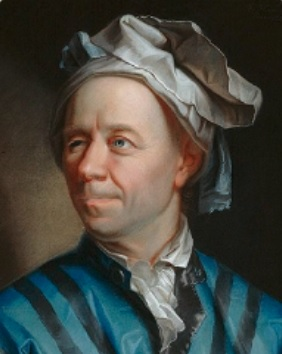
\includegraphics[width=\linewidth]{images/Euler.jpg}
\end{image}%
\tcblower
\end{figureptx}%
\end{subsectionptx}
%
%
\typeout{************************************************}
\typeout{Subseção 3.2.2 Exemplos introdutórios}
\typeout{************************************************}
%
\begin{subsectionptx}{Exemplos introdutórios}{}{Exemplos introdutórios}{}{}{g:subsection:idp150}
Vamos iniciar este tópico com dois exemplos para facilitar o entendimento do conceito de permutação caótica e também da demonstração.%
\begin{fact}{}{}{g:fact:idp151}%
Determine o número de permutações simples dos elementos \(a_1, a_2, . . . , a_n\), nas quais \(a_2\) está na segunda posição ou \(a_3\) está em terceira posição.%
\textbf{\blocktitlefont Solução}.\quad{}Definindo \(A_2\) como o conjunto das permutações em que \(a_2\) está em segunda posição e \(A_3\) como o conjunto das permutações em que \(a_3\) está em terceira posição, é fácil ver que%
\begin{equation*}
\#(A_{2})=\#(A_{3})=(n-1)!
\end{equation*}
e que%
\begin{equation*}
\#(A_{2}\cap A_{3})=(n-2)!.
\end{equation*}
Assim o número procurado nada mais é do que \(\#(A_{2} \cup A_{3})\) que é igual a:%
\begin{align*}
\#(A_2\cup A_3) = \amp ~ \#(A_2) + \#(A_3) - \#(A_2\cap A_3) \\
= \amp ~ (n-1)! + (n-1)!-(n-2)! \\
= \amp ~ 2\cdot(n-1)! - (n-2)! \\
= \amp ~ 2\cdot(n - 1)\cdot(n - 2)! - (n - 2)! \\
= \amp ~ (n-2)!\cdot(2n-2-1) \\
= \amp ~ (2n-3)\cdot(n-2)! 
\end{align*}
%
\end{fact}
\begin{fact}{}{}{x:fact:exem-antes-permut-cao}%
Dentre as permutações simples dos \(n\) elementos \(a_1, a_2, . . . , a_n\) determine o número daquelas em que \(a_2\) não está na segunda posição, \(a_3\) não está na terceira posição e nem \(a_4\) está na quarta posição.%
\textbf{\blocktitlefont Solução}.\quad{}Definimos \(A_i\), para \(i = 2, 3, 4\), como o conjunto das permutações em que \(a_i\) está no \(i\)-ésima posição, para \(i = 2, 3, 4\). Queremos encontrar o número de elementos no complementar de \(A_2\cup A_3\cup A_4\).%
\par
As cardinalidade dos conjuntos \(A_i's\) e das interseções dos \(A_i's\), dois a dois e três a três são:%
\par
\(\#(A_2) = \#(A_3) = \#(A_4) = (n-1)!;\)%
\par
\(\#(A_2\cap A_3) = \#(A_2\cap A_4) = \#(A_3\cap A_4) = (n-2)!;\)%
\par
\(\#(A_2\cap A_3\cap A_4) = (n-3)!.\)%
\par
Sabendo que o número total de permutações é \(n!\), a solução para o questionamento é%
\begin{gather*}
n!-\#(A_2)-\#(A_3)-\#(A_4)+\#(A_2\cap A_3)+  \\
~~~~~~~~~~~~~ +\#(A_2\cap A_4)+\#(A_3\cap A_4)-\#(A_2\cap A_3\cap A_4)
\end{gather*}
Que é igual a:%
\begin{equation*}
n!-3\times (n-1)!+3 \times (n-2)!-(n-3)! 
\end{equation*}
%
\end{fact}
\end{subsectionptx}
%
%
\typeout{************************************************}
\typeout{Subseção 3.2.3 Permutações Caóticas}
\typeout{************************************************}
%
\begin{subsectionptx}{Permutações Caóticas}{}{Permutações Caóticas}{}{}{g:subsection:idp152}
\begin{definition}{}{g:definition:idp153}%
Uma permutação de uma lista de \(n\) elementos é chamada de \emph{permutação caótica}, quando nenhum dos elementos da permutação está na posição original, ou seja, uma permutação de \(a_1,a_2, ...,a_n\)  é chamada de caótica quando nenhum dos \(a'_{i}s\) se encontra na \(i\)-ésima posição.%
\par
Notação:%
\begin{equation*}
D_n \text{ ou } D(n) 
\end{equation*}
%
\end{definition}
\begin{technology}{}{g:technology:idp154}%
As permutações caóticas dos elementos \(1, 2, 3, 4\) podem ser geradas no Sage, com o seguinte comando: \begin{sageinput}
Derangements(4).list()
\end{sageinput}
\begin{sageoutput}
[[2, 3, 4, 1],
 [4, 3, 1, 2],
 [2, 4, 1, 3],
 [3, 4, 2, 1],
 [3, 1, 4, 2],
 [4, 1, 2, 3],
 [4, 3, 2, 1],
 [3, 4, 1, 2],
 [2, 1, 4, 3]]
\end{sageoutput}
\end{technology}
\begin{technology}{}{x:technology:tec-caotica-r-sage}%
Todos os anagramas de AMOR, de forma que nenhuma letra fique na posição original. Troque as informações da lista para obter o número de permutações caóticas e as permutações caóticas da sua lista.%
\begin{sageinput}
D = Derangements(['A', 'M', 'O', 'R'])
print('número de permutações caóticas:', len(D))
print('todas as permutações caóticas:')
D.list()
\end{sageinput}
\begin{sageoutput}
número de permutações caóticas: 9
todas as permutações caóticas:
[['M', 'O', 'R', 'A'],
 ['R', 'O', 'A', 'M'],
 ['M', 'R', 'A', 'O'],
 ['O', 'R', 'M', 'A'],
 ['O', 'A', 'R', 'M'],
 ['R', 'A', 'M', 'O'],
 ['R', 'O', 'M', 'A'],
 ['O', 'R', 'A', 'M'],
 ['M', 'A', 'R', 'O']]
\end{sageoutput}
\end{technology}
\begin{theorem}{}{}{g:theorem:idp155}%
A quantidade de permutações caóticas de um conjunto com \(n\) elementos distintos, pode ser calculada da seguinte maneira:%
\begin{equation*}
D_n=n!\cdot\sum_{i=0}^{n}\dfrac{(-1)^i}{i!}.
\end{equation*}
%
\end{theorem}
\begin{proof}{}{g:proof:idp156}
Considere todas as permutações dos elementos \(a_1 , a_2 , \ldots , a_n\). Indicando por \(A_i\) todas as permutações formadas pelos elementos \(a_1 , a_2 , \ldots , a_n\) com \(a_i\) no \(i\)-ésimo lugar, calcularemos \(D_n\), usando a ideia do exemplo (\hyperref[x:fact:exem-antes-permut-cao]{Exemplo~{\xreffont\ref{x:fact:exem-antes-permut-cao}}}):%
\begin{align*}
D_n = \amp ~  n! - \sum_{i=1}^{n}\#A_i + \sum_{0\lt i\lt j\leq n}\#(A_i\cap A_j)+\cdots \\
\amp ~  \cdots  +(-1)^{n-1}\#(A_1\cap A_2\cap \cdots\cap A_n). 
\end{align*}
Visto que existem \(n\) termos no primeiro somatório, \(C_n^2\) termos no segundo, \(C_n^3\) termos no terceiro,\(\cdots\), \(C_n^n=1\) no último e%
\begin{align*}
\#(A_i) \amp =  (n-1)! \\
\#(A_i\cap A_j) \amp =  (n-2)! \\
\#(A_i\cap A_j\cap A_k) \amp =  (n-3)! \\
\vdots ~~~~~ \amp = ~~ \vdots \\
\#(A_1\cap A_2\cap\cdots\cap A_n) \amp =  1 
\end{align*}
temos%
\begin{align*}
D_n \amp = ~ n!-n\cdot(n-1)!+C_n^2\cdot(n-2)!-C_n^3\cdot(n-3)!+\cdots +(-1)^n\cdot 1 \\
\amp = ~ n!-\dfrac{n!}{1!}+\dfrac{n!}{2!}-\dfrac{n!}{3!}+\cdots
+(-1)^n\cdot \dfrac{n!}{n!} 
\end{align*}
evidenciando \(n!\), obtém-se:%
\begin{align*}
D_n \amp = ~ n!\cdot\left(1-\dfrac{1}{1!}+\dfrac{1}{2!}-\dfrac{1}{3!}+\cdots+(-1)^n\cdot \dfrac{1}{n!}\right) \\
\amp = ~ n!\cdot\sum_{i=0}^{n}\dfrac{(-1)^i}{i!} \qedhere
\end{align*}
%
\end{proof}
\begin{remark}{}{g:remark:idp157}%
Calculando o número de permutações caóticas no Sage: \leavevmode%
\begin{sageinput}
def D(n):
    d = 0
    for i in range(n+1):
        d = d + (-1)^(i)*(factorial(n)/factorial(i))
    return d
D(8)
\end{sageinput}
\begin{sageoutput}
14833
\end{sageoutput}
\end{remark}
\begin{fact}{}{}{g:fact:idp158}%
Luiz, Cláudia, Paulo, Rodrigo e Ana brincam entre si de amigo-secreto (ou amigo-oculto). O nome de cada um é escrito em um pedaço de papel, que é colocado em uma urna. Em seguida, cada participante da brincadeira retira da urna um dos pedaços de papel, ao acaso. De quantas formas pode ocorrer a distribuição dos papéis de modo que nenhum dos participantes retire seu próprio nome?%
\textbf{\blocktitlefont Solução}.\quad{}Uma clássica questão de permutação caótica, visto que durante a distribuição dos papéis nenhum dos participantes poderá retirar seu próprio nome. Assim o número de maneiras de ocorrer tal evento, é dado por:%
\begin{align*}
D_5 \amp = ~5!\cdot\left(1-\frac{1}{1!}+\frac{1}{2!}-\frac{1}{3!}+\frac{1}{4!}-\frac{1}{5!}\right) \\
\amp =  ~5!-5! + \frac{5!}{2!} -\frac{5!}{3!} + \frac{5!}{4!}-\frac{5!}{5!} \\
\amp =  ~5\cdot 4 \cdot 3 -5\cdot 4 + 5 - 1 \\
\amp = ~60-20+5-1 \\
\amp =  ~44 
\end{align*}
%
\end{fact}
\begin{fact}{}{}{g:fact:idp159}%
Quantas são as permutações de \((1, 2, 3, 4, 5, 6, 7, 8, 9, 10)\) que têm exatamente 4 elementos no seu lugar primitivo?%
\textbf{\blocktitlefont Solução}.\quad{}O número de modos de escolher os quatro elementos que ocuparão o seu lugar primitivo é \(C_{10}^4\).%
\par
Com estes elementos em seus lugares, os outros seis elementos devem ser arrumados de forma caótica. o que pode ser feito de \(D_6\) formas. A resposta é%
\begin{equation*}
C_{10}^4\times D_6 = 55650.
\end{equation*}
%
\end{fact}
\end{subsectionptx}
%
%
\typeout{************************************************}
\typeout{Subseção 3.2.4 Permutações Caóticas com Repetições}
\typeout{************************************************}
%
\begin{subsectionptx}{Permutações Caóticas com Repetições}{}{Permutações Caóticas com Repetições}{}{}{g:subsection:idp160}
Observe que a \hyperref[x:technology:tec-caotica-r-sage]{Tecnologia~{\xreffont\ref{x:technology:tec-caotica-r-sage}}} também faz o cálculo no caso de existirem elementos  repetidos, mas precisa listar todas as possibilidades, dependendo da quantidade de permutações o cálculo pode demorar.%
\par
Esta seção ainda não está pronta, mas a \hyperref[x:technology:tec-caotica-r]{Tecnologia~{\xreffont\ref{x:technology:tec-caotica-r}}} já está funcionando e usa um algoritmo eficiente, fazendo o cálculo via polinômios de torre.%
\begin{technology}{Faça você mesmo.}{x:technology:tec-caotica-r}%
\begin{figureptx}{Número de Permutações Caóticas podendo ter elementos repetidos.}{x:figure:interactive-caotica-r}{}%
\centering
O número de anagramas da palavra MATEMATICA, de forma que nenhuma letra fique na posição original, ou seja, o número de permutações caóticas. Troque as informações da lista para obter o número de permutações caóticas da sua lista.%
\setlength{\qrsize}{9em}
\setlength{\previewwidth}{\linewidth}
\addtolength{\previewwidth}{-\qrsize}
\begin{tcbraster}[raster columns=2, raster column skip=1pt, raster halign=center, raster force size=false, raster left skip=0pt, raster right skip=0pt]%
\begin{tcolorbox}[previewstyle, width=\previewwidth]%
\IfFileExists{images/interactive-caotica-r-preview.png}%
{\includegraphics[width=0.80\linewidth,height=\qrsize,keepaspectratio]{images/interactive-caotica-r-preview.png}}%
{\small{}Specify static image with \mono{@preview} attribute,\\Or create and provide automatic screenshot as \mono{images/interactive-caotica-r-preview.png} via the \mono{mbx} script}%
\end{tcolorbox}%
\begin{tcolorbox}[qrstyle]%
{\hypersetup{urlcolor=black}\qrcode[height=\qrsize]{/interactive-caotica-r.html}}%
\end{tcolorbox}%
\end{tcbraster}%
\tcblower
\end{figureptx}%
\end{technology}
\end{subsectionptx}
%
%
\typeout{************************************************}
\typeout{Exercícios 3.2.5 Exercícios}
\typeout{************************************************}
%
\begin{exercises-subsection}{Exercícios}{}{Exercícios}{}{}{g:exercises:idp161}
\begin{divisionexercise}{1}{}{}{g:exercise:idp162}%
Suponha que \(\#A=n\). Quantas são as funções \(f:A\rightarrow A\) para as quais a equação \(f(x)=x\) não possui solução? Quantas são as funções \(f:A\rightarrow A\) \terminology{bijetoras} para as quais a equação \(f(x)=x\) não possui solução?%
\par\smallskip%
\noindent\textbf{\blocktitlefont Resposta}.\hypertarget{g:answer:idp163}{}\quad{}a) \((n-1)^n\), b) \(D_n\).%
\end{divisionexercise}%
\begin{divisionexercise}{2}{}{}{g:exercise:idp164}%
Quantas são as permutações de \((1, 2, 3, 4, 5, 6, 7, 8, 9, 10, 11, 12)\) que têm exatamente 5 elementos no seu lugar primitivo?%
\par\smallskip%
\noindent\textbf{\blocktitlefont Resposta}.\hypertarget{g:answer:idp165}{}\quad{}1468368%
\end{divisionexercise}%
\begin{divisionexercise}{3}{}{}{g:exercise:idp166}%
Determine o número de permutações caóticas de \((1, 2, 3, 4, 5, 6, 7, 8, 9, 10, 11, 12)\) nas quais os números \(1, 2, 3, 4, 5\) ocupam, em alguma ordem, os cinco primeiro lugares.%
\par\smallskip%
\noindent\textbf{\blocktitlefont Resposta}.\hypertarget{g:answer:idp167}{}\quad{}81576%
\end{divisionexercise}%
\begin{divisionexercise}{4}{}{}{g:exercise:idp168}%
Uma empresa tem sete estagiárias. Cada uma delas deve cumprir três horas de trabalho semanais, sendo duas horas no turno da manhã e uma no turno da tarde. De quantas maneiras o Recursos Humanos pode montar a agenda de trabalho semanal (segunda a domingo) desses estagiárias, de modo que todas cumpram as três horas semanais, trabalhando diariamente apenas em um turno?%
\par\smallskip%
\noindent\textbf{\blocktitlefont Resposta}.\hypertarget{g:answer:idp169}{}\quad{}9344160%
\end{divisionexercise}%
\end{exercises-subsection}
\end{sectionptx}
%
%
\typeout{************************************************}
\typeout{Seção 3.3 Os Lemas de Kaplansky}
\typeout{************************************************}
%
\begin{sectionptx}{Os Lemas de Kaplansky}{}{Os Lemas de Kaplansky}{}{}{x:section:section-lemas-kaplansky}
\begin{objectives}{Objetivos}{x:objectives:objetivos-permutacao-caotica}
%
\begin{enumerate}
\item{}Nota Histórica.%
\item{}Enunciar e demonstrar os lemas de Kaplansky.%
\item{}Exemplificar.%
\item{}Calcular no Sage, o número de subconjuntos satisfazendo os Lemas de Kaplansky.%
\end{enumerate}
\end{objectives}
%
%
\typeout{************************************************}
\typeout{Subseção 3.3.1 Nota Histórica}
\typeout{************************************************}
%
\begin{subsectionptx}{Nota Histórica}{}{Nota Histórica}{}{}{g:subsection:idp170}
Irving Kaplansky, matemático americano, nasceu em 22 de março de 1917 em Toronto e faleceu em 25 de junho de 2006. O talentoso matemático publicou o artigo "Solution of the problème des ménages"  no Boletim da Sociedade Americana de Matemática em 1943, com uma solução para o afamado Problema de Lucas.%
\par
Kaplansky foi para a Universidade de Harvard e recebeu seu Ph.D. lá em 1941, trabalhando com Saunders MacLane. Ele foi instrutor de Benjamin Peirce em Harvard de 1941 a 1944 e, em seguida, ingressou no Grupo de Matemática Aplicada fazendo trabalhos de guerra na Universidade de Columbia de 1944 a 1945.%
\par
Seu trabalho foi bastante extenso na matemática, incluindo desde áreas da álgebra até grandes contribuições na Teoria dos Anéis, Teoria dos Grupos e Teoria dos Corpos. Publicou muitos artigos e trabalhou com diversos coautores.%
\begin{figureptx}{Irving Kaplansky, fonte: www.ams.org}{x:figure:figura-kaplansky}{}%
\begin{image}{0.35}{0.3}{0.35}%
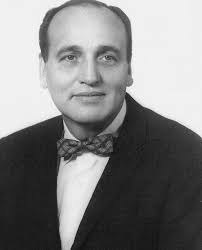
\includegraphics[width=\linewidth]{images/Kaplansky.jpg}
\end{image}%
\tcblower
\end{figureptx}%
\end{subsectionptx}
%
%
\typeout{************************************************}
\typeout{Subseção 3.3.2 O 1º Lema de Kaplansky}
\typeout{************************************************}
%
\begin{subsectionptx}{O 1º Lema de Kaplansky}{}{O 1º Lema de Kaplansky}{}{}{g:subsection:idp171}
\begin{introduction}{}%
Para mostrar os benefícios dos Lemas de Kaplansky, iniciaremos a seção com o exemplo a seguir:%
\end{introduction}%
\begin{fact}{}{}{g:fact:idp172}%
De quantos maneiras podemos formar um subconjunto com 4 elementos, do conjunto%
\begin{equation*}
A=\{a,b,c,d,e,f,g,h\},
\end{equation*}
de modo que não possuam duas letras que ocupem posições consecutivas no alfabeto?%
\textbf{\blocktitlefont Solução}.\quad{}Esse problema será resolvido criando uma forma alternativa de representar os subconjuntos onde marcaremos com o sinal \((+)\) os elementos pertencente ao subconjunto e com o sinal \((-)\) os elementos que não pertencentes ao subconjunto.%
\begin{equation*}
\{a,c,e,h\} \text{ será representado  por } +-+-+--+
\end{equation*}
%
\begin{equation*}
\{b,d,f,h\} \text{ será representado  por } -+-+-+-+
\end{equation*}
%
\begin{equation*}
\{b,e,g,h\} \text{ será representado  por } -+--+-++
\end{equation*}
O terceiro caso não satisfaz as condições do enunciado, pois 2 \((+)\) juntos significa que teremos letras consecutivas (do alfabeto).%
\par
Assim, compreendendo o problema observa-se que para soluciona-lo devemos calcular o número de formas distintas de permutar 8 símbolos, onde \(4\) são \((-)\) e 4 são \((+)\) de modo que não tenha 2 símbolos \((+)\) juntos.%
\begin{equation*}
\LARGE \bigcirc-\bigcirc-\bigcirc-\bigcirc-\bigcirc
\end{equation*}
Veja que de acordo com  o esquema, de círculos e traços, podem-se colocar 4 símbolos \((+)\) em quaisquer dos cinco lugares, ou seja, é possível escolher 4 dos 5 lugares disponíveis (representados pelas circunferências) para por os símbolos \((+)\) o que pode ser realizado de%
\begin{equation*}
C_5^4=5 \text{ modos distintos}.
\end{equation*}
Dessa forma 5 subconjuntos podem ser formados, os quais estão listados abaixo:%
\begin{equation*}
\{ a, c, e, g \}, \{ a, c, e, h \}, \{ a, c, f, h \}, \{ a, d, f, h \}, \{ b, d, f, h \} 
\end{equation*}
%
\end{fact}
\begin{theorem}{}{}{g:theorem:idp173}%
\terminology{(1º Lema de Kaplansky)} O número de subconjuntos com \(p\) elementos de \(\{1,2,3,\cdots,n\}\) nos quais não há números consecutivos é:%
\begin{equation*}
K(n,p)=C_{n-p+1}^p.
\end{equation*}
%
\end{theorem}
\begin{proof}{}{g:proof:idp174}
Deseja-se formar subconjuntos formados por \(p\) elementos não consecutivos. De acordo com o exemplo anterior, os elementos desse subconjunto serão representados com o símbolo \((+)\).%
\par
Assim teremos \((n-p)\) elementos que serão apresentados com o símbolo \((-)\), que retratam os números que não estarão no subconjunto. Entre os símbolos \((-)\) existirão \((n-p+1)\) espaços vazios disponíveis. Desta forma resta escolher entre os \((n-p+1)\) espaços vazios aqueles que serão ocupados pelos símbolos \((+)\). Logo,%
\begin{equation*}
K(n,p)=C_{n-p+1}^p.\qedhere
\end{equation*}
%
\end{proof}
\begin{remark}{}{g:remark:idp175}%
Calculando \(K(8, 5)\) no Sage:%
\begin{sageinput}
K(n, p) = binomial(n-p+1, p) 
K(8, 4)
\end{sageinput}
\begin{sageoutput}
5
\end{sageoutput}
\end{remark}
\begin{technology}{Faça você mesmo.}{g:technology:idp176}%
\begin{figureptx}{Todos os subconjuntos com \(p\) elementos.}{x:figure:interactive-kaplansky2}{}%
\centering
Escolha uma lista de letras ou números e \(p\) para obter os subconjuntos da lista com \(p\) elementos, nos quais não há elementos, da lista, consecutivos.%
\setlength{\qrsize}{9em}
\setlength{\previewwidth}{\linewidth}
\addtolength{\previewwidth}{-\qrsize}
\begin{tcbraster}[raster columns=2, raster column skip=1pt, raster halign=center, raster force size=false, raster left skip=0pt, raster right skip=0pt]%
\begin{tcolorbox}[previewstyle, width=\previewwidth]%
\IfFileExists{images/interactive-kaplansky2-preview.png}%
{\includegraphics[width=0.80\linewidth,height=\qrsize,keepaspectratio]{images/interactive-kaplansky2-preview.png}}%
{\small{}Specify static image with \mono{@preview} attribute,\\Or create and provide automatic screenshot as \mono{images/interactive-kaplansky2-preview.png} via the \mono{mbx} script}%
\end{tcolorbox}%
\begin{tcolorbox}[qrstyle]%
{\hypersetup{urlcolor=black}\qrcode[height=\qrsize]{/interactive-kaplansky2.html}}%
\end{tcolorbox}%
\end{tcbraster}%
\tcblower
\end{figureptx}%
\end{technology}
\begin{fact}{}{}{g:fact:idp177}%
Um exame vestibular se constitui de 10 questões distintas, 3 das quais da área de Matemática. Determine de quantas formas é possível programar a sequência das 10 questões, de maneira que duas questões da área de Matemática não se sucedam.%
\textbf{\blocktitlefont Solução}.\quad{}São 3 questões de Matemática e 7 questões de outras áreas \((Q_1, Q_2,\cdots, Q_7)\). Inicialmente, iremos dispor as provas que não sofrem restrições.%
\begin{equation*}
\large\bigcirc \ Q_1\ \bigcirc \ Q_2 \ \bigcirc \ Q_3 \ \bigcirc \ Q_4 \ \bigcirc \ Q_5 \ \bigcirc \ Q_6 \  \bigcirc \ Q_7 \ \bigcirc
\end{equation*}
%
\par
Temos 8 lugares \(\bigcirc\) para colocar as 3 provas de Matemática e o número de formas de calcular isso, pode ser feito utilizando o 1º Lema de Kaplansky:%
\begin{equation*}
K(10,3).
\end{equation*}
Devemos, agora, permutar a ordem das 7 provas das outras áreas e as 3 de Matemática. Assim, temos%
\begin{equation*}
7! \times 3! \text{ possibilidades.}
\end{equation*}
E o total de formas de programar a sequência dessas 10 provas é:%
\begin{equation*}
K(10, 3)\times 7! \times 3! = 1693440. 
\end{equation*}
%
\end{fact}
\end{subsectionptx}
%
%
\typeout{************************************************}
\typeout{Subseção 3.3.3 O 2º Lema de Kaplansky}
\typeout{************************************************}
%
\begin{subsectionptx}{O 2º Lema de Kaplansky}{}{O 2º Lema de Kaplansky}{}{}{g:subsection:idp178}
\begin{theorem}{}{}{g:theorem:idp179}%
\terminology{(2º Lema de Kaplansky)} O número de subconjuntos com \(p\) elementos de \(\{1,2,3,\cdots,n\}\) nos quais não há números consecutivos e, 1 e \(n\) são consecutivos, é :%
\begin{equation*}
KC(n,p)=\frac{n}{n-p}\times C_{n-p}^p.
\end{equation*}
%
\end{theorem}
\begin{proof}{}{g:proof:idp180}
O problema será dividido em dois casos:%
\par
\terminology{1º Caso:} O elemento 1 pertencendo ao subconjunto composto por \(p\) elementos. Neste caso, será feito a análise de quantos formas poderá serão escolhidos os outros \(p-1\) elementos do conjunto \(\{3,4,5,\cdots,n-1\}\), pois os elementos 1 e \(n\) não podem pertencer ao conjunto. Dessa forma, utilizando o 1º lema de Kaplansky, o número de maneiras que isso pode ocorrer é:%
\begin{equation*}
K(n-3,p-1)=C^{p-1}_{n-p-1}=\dfrac{(n-p-1)!}{(n-2p)!\cdot(p-1)!}.
\end{equation*}
%
\par
\terminology{2º Caso:} O elemento 1 não pertencendo ao subconjunto composto por \(p\) elementos. Nesse caso a escolha de \(p\) elementos será realizado entre os elementos do conjunto \(\{2,3,4,...n\}\). No entanto pelo primeiro lema de Kaplansky a escolha será determinada por%
\begin{equation*}
K(n-1,p)=C^p_{n-p}=\dfrac{(n-p)!}{(n-2p)!\cdot p!}
\end{equation*}
%
\par
Pelo Princípio Aditivo, somando os resultados do 1º e do 2º caso, a solução do problema será dado por:%
\begin{align*}
KC(n,p) = \amp ~\dfrac{(n-p-1)!}{(n-2p)!\cdot(p-1)!}+\dfrac{(n-p)!}{(n-2p)!\cdot p!} \\
=\amp ~ \dfrac{p\cdot (n-p-1)!+(n-p)\cdot(n-p-1)!}{{(n-2p)!\cdot p!}} \\
=\amp ~ \dfrac{(n-p-1)!n}{{(n-2p)!\cdot p!}} \\
=\amp ~ \dfrac{n-p}{n-p}\cdot\dfrac{(n-p-1)!n}{(n-2p)!\cdot p!} \\
=\amp ~ \dfrac{n}{n-p}\cdot\dfrac{(n-p)!}{(n-2p)!\cdot p!} 
\end{align*}
finalmente,%
\begin{equation*}
KC(n,p)=\dfrac{n}{n-p}\cdot C^p_{n-p}.\qedhere
\end{equation*}
%
\end{proof}
\begin{fact}{}{}{g:fact:idp181}%
Débora deseja correr 3 vezes por semana durante esse bimestre. De quantas formas ela poderá escolher os dias da corrida, se Débora não deseja correr em dias consecutivos?%
\textbf{\blocktitlefont Solução}.\quad{}Nesta  questão observa-se que a disposição dos dias da semana geram um sistema cíclico, ou seja, o início de uma semana dá continuação ao fim da semana anterior a ela e assim sucessivamente, como pode ser verificado na figura abaixo:%
\begin{figureptx}{Dias da semana.}{x:figure:semana}{}%
\begin{image}{0.3}{0.4}{0.3}%
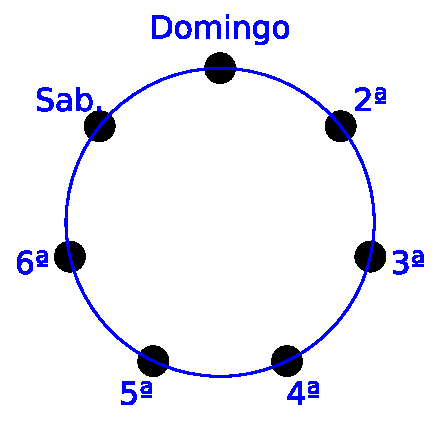
\includegraphics[width=\linewidth]{images/semana}
\end{image}%
\tcblower
\end{figureptx}%
Desta forma, Débora deve escolher 3 dias entre: domingo, segunda, terça, quarta, quinta, sexta e sábado de maneira que não apareçam dois dias consecutivos. O número de maneiras que Débora pode escolher os 3 dias é:%
\begin{equation*}
KC(7, 3) = 7.
\end{equation*}
%
\end{fact}
\begin{fact}{}{}{g:fact:idp182}%
Dado um decágono, quantos são os triângulos cujos vértices são vértices não consecutivos do decágono?%
\textbf{\blocktitlefont Solução}.\quad{}O resultado esperado corresponde a escolha de 3 elementos não consecutivos de um conjunto de 10 elementos (vértices), como eles estão organizados de forma circular, tem-se:%
\begin{equation*}
KC(10, 3) = 50.
\end{equation*}
%
\end{fact}
\begin{remark}{}{g:remark:idp183}%
Calculando \(KC(7, 3)\) no Sage:%
\begin{sageinput}
KC(n, p) = (n/(n-p))*binomial(n-p, p) 
KC(7, 3)
\end{sageinput}
\begin{sageoutput}
7
\end{sageoutput}
\end{remark}
\begin{technology}{Faça você mesmo.}{g:technology:idp184}%
\begin{figureptx}{Todos os subconjuntos com \(p\) elementos.}{x:figure:interactive-kaplansky4}{}%
\centering
Escolha uma lista de letras ou números e \(p\) para obter os subconjuntos da lista com \(p\) elementos, nos quais não há elementos, da lista, consecutivos, considerando o primeiro e o último consecutivos.%
\setlength{\qrsize}{9em}
\setlength{\previewwidth}{\linewidth}
\addtolength{\previewwidth}{-\qrsize}
\begin{tcbraster}[raster columns=2, raster column skip=1pt, raster halign=center, raster force size=false, raster left skip=0pt, raster right skip=0pt]%
\begin{tcolorbox}[previewstyle, width=\previewwidth]%
\IfFileExists{images/interactive-kaplansky4-preview.png}%
{\includegraphics[width=0.80\linewidth,height=\qrsize,keepaspectratio]{images/interactive-kaplansky4-preview.png}}%
{\small{}Specify static image with \mono{@preview} attribute,\\Or create and provide automatic screenshot as \mono{images/interactive-kaplansky4-preview.png} via the \mono{mbx} script}%
\end{tcolorbox}%
\begin{tcolorbox}[qrstyle]%
{\hypersetup{urlcolor=black}\qrcode[height=\qrsize]{/interactive-kaplansky4.html}}%
\end{tcolorbox}%
\end{tcbraster}%
\tcblower
\end{figureptx}%
\end{technology}
\end{subsectionptx}
%
%
\typeout{************************************************}
\typeout{Exercícios 3.3.4 Exercícios}
\typeout{************************************************}
%
\begin{exercises-subsection}{Exercícios}{}{Exercícios}{}{}{g:exercises:idp185}
\begin{divisionexercise}{1}{}{}{g:exercise:idp186}%
Um estacionamento tem 10 vagas, uma ao lado da outra, inicialmente todas livres. Um carro preto, um carro rosa e um carro branco chegam a esse estacionamento. De quantas maneiras diferentes esses carros podem ocupar três vagas de forma que haja pelo menos uma vaga livre entre eles?%
\par\smallskip%
\noindent\textbf{\blocktitlefont Resposta}.\hypertarget{g:answer:idp187}{}\quad{}336%
\end{divisionexercise}%
\begin{divisionexercise}{2}{}{}{g:exercise:idp188}%
De quantos modos podemos formar uma sequência de 9 elementos iguais a 1 e 6 elementos iguais a 0 se dois elementos iguais a 0 não podem ser adjacentes?%
\par\smallskip%
\noindent\textbf{\blocktitlefont Resposta}.\hypertarget{g:answer:idp189}{}\quad{}210%
\end{divisionexercise}%
\begin{divisionexercise}{3}{}{}{g:exercise:idp190}%
(ITA) 12 cavaleiros estão sentados em torno de uma mesa redonda. Cada um dos 12 cavaleiros considera seus dois vizinhos como rivais. Deseja-se formar um grupo de 5 cavaleiros para libertar uma princesa. Nesse grupo não poderá haver cavaleiros rivais. Determine de quantas maneiras é possível escolher esse grupo.%
\par\smallskip%
\noindent\textbf{\blocktitlefont Resposta}.\hypertarget{g:answer:idp191}{}\quad{}36%
\end{divisionexercise}%
\begin{divisionexercise}{4}{}{}{g:exercise:idp192}%
8 pessoas devem se sentar em 25 cadeiras colocadas em torno de uma mesa circular. De quantos modos isso pode ser feito se não deve haver ocupação simultânea de duas cadeiras adjacentes?%
\par\smallskip%
\noindent\textbf{\blocktitlefont Resposta}.\hypertarget{g:answer:idp193}{}\quad{}1441440000%
\end{divisionexercise}%
\end{exercises-subsection}
\end{sectionptx}
%
%
\typeout{************************************************}
\typeout{Seção 3.4 Princípio da Casa dos Pombos}
\typeout{************************************************}
%
\begin{sectionptx}{Princípio da Casa dos Pombos}{}{Princípio da Casa dos Pombos}{}{}{x:section:section-casa-pombos}
\begin{objectives}{Objetivos}{x:objectives:objetivos-permutacao-caotica}
%
\begin{enumerate}
\item{}Nota Histórica.%
\item{}Enunciar e demonstrar o Princípio da Casa dos Pombos.%
\item{}Exemplificar.%
\end{enumerate}
\end{objectives}
%
%
\typeout{************************************************}
\typeout{Subseção 3.4.1 Nota Histórica}
\typeout{************************************************}
%
\begin{subsectionptx}{Nota Histórica}{}{Nota Histórica}{}{}{g:subsection:idp194}
O Princípio da Casa dos Pombos, também conhecido como O Princípio das Gavetas de Dirichlet, surgiu em 1834, o conceito foi utilizado pelo matemático alemão Johann Peter Gustav Lejeune Dirichlet, estudante da Universidade de Paris, que trabalhou nas Universidades de Breslau e Berlim, posteriormente sendo escolhido como sucessor de Johann Carl Friedrich Gauss na Universidade de Göttingen. Dirichlet foi responsável por grandes avanços na Matemática, especialmente na área de Teoria dos Números.%
\begin{figureptx}{Johann Peter Gustav Lejeune Dirichlet, fonte: gigantesdamatematica.wordpress.com\slash{}}{x:figure:figura-dirichlet}{}%
\begin{image}{0.35}{0.3}{0.35}%
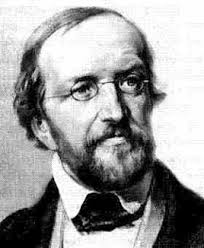
\includegraphics[width=\linewidth]{images/Dirichlet.jpg}
\end{image}%
\tcblower
\end{figureptx}%
\end{subsectionptx}
%
%
\typeout{************************************************}
\typeout{Subseção 3.4.2 1ª versão do Princípio da Casa dos Pombos}
\typeout{************************************************}
%
\begin{subsectionptx}{1ª versão do Princípio da Casa dos Pombos}{}{1ª versão do Princípio da Casa dos Pombos}{}{}{g:subsection:idp195}
\begin{theorem}{}{}{g:theorem:idp196}%
Se \(k+1\) pombos forem colocados em \(k\) casas, então existe pelo menos uma casa contendo dois ou mais pombos.%
\end{theorem}
\begin{proof}{}{g:proof:idp197}
Suponha que nenhuma das \(k\) casas contém mais de um pombo. Então o número total de pombos seria no máximo \(k\). Isto é uma contradição, já que existem pelo menos \(k+1\) pombos.\end{proof}
\begin{remark}{}{g:remark:idp198}%
Podemos interpretar o princípio usando funções da seguinte forma: Sejam \(\mathcal{P}\) e \(\mathcal{C}\), dois conjuntos. Se o número de elementos de \(\mathcal{P}\) for maior que o números de elementos de \(\mathcal{C}\), então não existe uma função injetiva de \(\mathcal{P}\) para \(\mathcal{C}\), ou seja, pelo menos dois elementos do domínio terão a mesma imagem, independente da função entre \(\mathcal{P}\) e \(\mathcal{C}\).%
\par
Essencialmente, para usar este princípio, precisamos identificar dois conjuntos, que chamaremos sugestivamente de \(\mathcal{P}\) e \(\mathcal{C}\) para representarem o conjunto dos pombos e o conjunto das casas, respectivamente. Em seguida comparamos o número de elementos entre eles.%
\end{remark}
\begin{fact}{}{}{g:fact:idp199}%
Mostre que, em um grupo de 367 pessoas, pelo menos duas fazem o aniversário no mesmo dia.%
\textbf{\blocktitlefont Solução}.\quad{}Chame de \(\mathcal{P}\) o conjunto das pessoas e \(\mathcal{C}\) o conjunto dos dias do ano. Desta forma como temos mais elementos em \(\mathcal{P}\) do que em \(\mathcal{C}\), pelo princípio da casa dos pombos, pelo menos duas pessoas fazem aniversário no mesmo dia.%
\end{fact}
\begin{fact}{}{}{g:fact:idp200}%
Mostre que entre nove números que não possuem divisores primos maiores que cinco, existem dois cujo produto é um quadrado.%
\textbf{\blocktitlefont Solução}.\quad{}Inicialmente observe que, qualquer número inteiro que não possui divisor primo maior que cinco, se escreve na forma \(2^a3^b5^c\), com \(a, b\) e \(c \in \mathbb{N}\).%
\par
Defina um conjunto com 9 números arbitrários, que satisfaça as hipóteses do enunciado:%
\begin{equation*}
\mathcal{P} = \{ 2^{a_1}3^{b_1}5^{c_1}, 2^{a_2}3^{b_2}5^{c_2}, \ldots, 2^{a_9}3^{b_9}5^{c_9} \}.
\end{equation*}
Como os expoentes \(a_i, b_i\) e \(c_i\) só podem ser pares ou ímpares, seja \(\mathcal{C}\) um conjunto que represente todas as paridades possíveis para os expoentes de 2, 3 e 5 em \(2^a3^b5^c\). Este conjunto possui 8 elementos, pois temos duas possibilidades para a paridade de cada um dos 3 expoentes.%
\par
Como o conjunto \(\mathcal{P}\) é formado por nove elementos, pelo princípio da casa dos pombos, teremos dois elementos em \(\mathcal{P}\), cujos expoentes possuem a mesma paridade, digamos que \(2^{a_i}3^{b_i}5^{c_i}\) e \(2^{a_j}3^{b_j}5^{c_j}\).%
\par
O produto entre eles é da forma \(2^{a_i+a_j}3^{b_i+b_j}5^{c_i+c_j}=2^{2x}3^{2y}5^{2z}\), com \(x, y, z \in \mathbb{N}\), que é um quadrado, pois pode ser escrito na forma%
\begin{equation*}
(2^{x}3^{y}5^{z})^2\text{.}
\end{equation*}
%
\end{fact}
\begin{fact}{}{}{g:fact:idp201}%
Prove que, de qualquer conjunto de dez números naturais distintos de dois dígitos, podemos escolher dois subconjuntos A e B (disjuntos) cuja a soma dos elementos é a mesma em ambos.%
\textbf{\blocktitlefont Solução}.\quad{}Seja \(S\) um conjunto com 10 números naturais distintos de dois dígitos. A soma de todos os elementos de \(S\) pode ser no máximo 945, no caso em que \(S=\{90, 91, \ldots, 99\}\).%
\par
Considere o conjunto das partes de \(S\), ou seja, o conjunto formado por todos os subconjuntos de \(S\). Este conjunto possui \(2^{10}\) elementos, sendo um deles o conjunto vazio, pois para formar um subconjunto de \(S\), precisamos decidir se cada elemento de \(S\) vai pertencer ou não a este subconjunto.%
\par
Defina \(\mathcal{C} = \{ 1, 2, \ldots, 945 \}\) e \(\mathcal{P}\) como o conjunto das partes de \(S\), menos o conjunto vazio. Desta forma \(\mathcal{P}\) possui \(2^{10}-1 = 1023\) elementos.%
\par
Observe que um elemento de \(\mathcal{P}\) é um subconjunto de \(S\) e que a soma dos elementos de um elemento de \(\mathcal{P}\) será um número que pertence a \(\mathcal{C}\). Pelo princípio da casa dos pombos, como temos mais elementos em \(\mathcal{P}\) do que em \(\mathcal{C}\), pelo menos dois elementos \(A, B \in \mathcal{P}\) possuem a mesma soma.%
\par
Se \(A\) e \(B\) forem disjuntos, acabou. Se não, considere \(A' = A- A\cap B\) e \(B' = B - A \cap B\). Logo, os conjuntos \(A'\) e \(B'\) são disjuntos e a soma dos seus elementos é a mesma.%
\end{fact}
\end{subsectionptx}
%
%
\typeout{************************************************}
\typeout{Subseção 3.4.3 2ª versão do Princípio da Casa dos Pombos}
\typeout{************************************************}
%
\begin{subsectionptx}{2ª versão do Princípio da Casa dos Pombos}{}{2ª versão do Princípio da Casa dos Pombos}{}{}{g:subsection:idp202}
\begin{remark}{}{g:remark:idp203}%
Para uma versão mais geral do princípio da casa dos pombos, vamos usar a função teto%
\begin{equation*}
\lceil ~ \rceil: \mathbb{R}\rightarrow \mathbb{Z}
\end{equation*}
dada por%
\begin{equation*}
\lceil x\rceil = \min\{ z\in \mathbb{Z} | z\geq x \},
\end{equation*}
ou seja, é o menor inteiro que é maior ou igual a \(x\). Observe que \(\lceil x \rceil \lt x +1 \), para qualquer \(x \in \mathbb{R}\).%
\end{remark}
\begin{fact}{}{}{g:fact:idp204}%
%
\begin{equation*}
\lceil \frac{1}{2} \rceil = 1, \lceil 3.1 \rceil = 4, \lceil -\frac{1}{2} \rceil=0.
\end{equation*}
%
\end{fact}
\begin{theorem}{}{}{g:theorem:idp205}%
Se \(n\) pombos forem colocados em \(k\) casas, então existe pelo menos uma casa contendo pelo menos%
\begin{equation*}
\left\lceil \frac{n}{k} \right\rceil 
\end{equation*}
pombos.%
\end{theorem}
\begin{proof}{}{g:proof:idp206}
Suponha que nenhuma das caixas contém mais que \(\left\lceil \frac{n}{k} \right\rceil-1\) pombos. Então, o número total de pombos é no máximo%
\begin{equation*}
k\left(\left\lceil \frac{n}{k} \right\rceil-1\right) \lt k\left( \left( \frac{n}{k} +1 \right) -1 \right) = n, 
\end{equation*}
na qual a desigualdade \(\left\lceil \frac{n}{k} \right\rceil \lt  \frac{n}{k} +1 \) foi usada. Esta é uma contradição, pois existem um total de \(n\) pombos.%
\end{proof}
\begin{fact}{}{}{g:fact:idp207}%
Nove pontos são colocados no interior de um triângulo de área 4\(cm^2\), de forma que não tenha 3 pontos colineares. Mostre que podemos escolher três deles para serem os vértices de um triângulo de área no máximo igual a 1\(cm^2\).%
\textbf{\blocktitlefont Solução}.\quad{}Sejam \(A, B\) e \(C\) os vértices do triângulo de área 4\(cm^2\). Considere três pontos \(D_1, D_2\) e \(D_3\) na arestas \(BC\), de forma que \(ABD_1, AD_1D_2,  AD_2D_3\) e \(AD_3C\) formem quatro triângulos, cada um com área de 1\(cm^2\).%
\par
Desta forma ao colocar os pontos no triâgulo \(ABC\), pelo princípio da casa dos pombos, existem pelo menos \(\lceil 9/4 \rceil = 3\) pontos em um dos quatro triângulos: \(ABD_1, AD_1D_2,  AD_2D_3\) e \(AD_3C\).%
\begin{figureptx}{Triângulo subdividido.}{x:figure:triang}{}%
\begin{image}{0.35}{0.3}{0.35}%
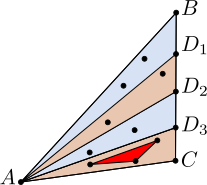
\includegraphics[width=\linewidth]{images/triang}
\end{image}%
\tcblower
\end{figureptx}%
Logo os três pontos que estão dentro de um destes 4 triângulos, por não serem colineares, formam um triângulo de área no máximo igual a 1\(cm^2\).%
\end{fact}
\begin{fact}{}{}{g:fact:idp208}%
Assuma que em um grupo de 6 pessoas, cada par de pessoas consistem em dois amigos ou dois inimigos. Mostre que ou existem 3 amigos mútuos ou 3 inimigos mútuos.%
\textbf{\blocktitlefont Solução}.\quad{}Seja \(A\) uma das 6 pessoas. Sejam \(\mathcal{C}=\{\{\mbox{amigo de }A\}, \{\mbox{inimigo de }A\}\}\) e \(\mathcal{P} = \{B, C, D, E, F\}\) o conjunto com as outras 5 pessoas.%
\par
Pela 2ª versão do princípio da casa dos pombos, dividindo as 5 pessoas de \(\mathcal{P}\) nos 2 conjuntos de \(\mathcal{C}\), um desses conjuntos possui pelo menos  \(\lceil 5/2 \rceil = 3\) elementos. Então, ou existem 3 ou mais que são amigos de \(A\), ou 3 ou mais que são inimigos de \(A\).%
\par
Suponha sem perda de generalidade que \(B, C\) e \(D\) sejam amigos de \(A\). Se quaisquer duas destas 3 pessoas são amigas, então estas duas pessoas e \(A\) formam um conjunto de 3 amigos mútuos.%
\end{fact}
\end{subsectionptx}
%
%
\typeout{************************************************}
\typeout{Exercícios 3.4.4 Exercícios}
\typeout{************************************************}
%
\begin{exercises-subsection}{Exercícios}{}{Exercícios}{}{}{g:exercises:idp209}
\begin{divisionexercise}{1}{}{}{g:exercise:idp210}%
Qual é o número mínimo de pessoas que deve haver em um grupo para que possamos garantir que nele haja pelo menos 5 pessoas nascidas no mesmo mês?%
\par\smallskip%
\noindent\textbf{\blocktitlefont Resposta}.\hypertarget{g:answer:idp211}{}\quad{}49%
\end{divisionexercise}%
\begin{divisionexercise}{2}{}{}{g:exercise:idp212}%
A comissão organizadora de um congresso dividiu os 75 professores presentes em 8 grupos, de acordo com a disciplina ministrada pelo professor. Sabendo que cada um deles ministra uma única disciplina, mostre que haverá pelo menos um grupo com no mı́nimo 10 professores.%
\end{divisionexercise}%
\begin{divisionexercise}{3}{}{}{g:exercise:idp213}%
Escolhem-se ao acaso 5 pontos sobre a superfície de um quadrado de lado 2. Mostre que pelo menos um dos segmentos que eles determinam tem comprimento menor ou igual a \(\sqrt{2}\).%
\end{divisionexercise}%
\begin{divisionexercise}{4}{}{}{g:exercise:idp214}%
Prove que todo número natural tem um múltiplo que se escreve, na base 10, apenas com os algarismos 0 e 1.%
\end{divisionexercise}%
\begin{divisionexercise}{5}{}{}{g:exercise:idp215}%
Prove que em qualquer conjunto de 52 inteiros existe um par de inteiros cuja soma ou cuja diferença é divisível por 100.%
\end{divisionexercise}%
\end{exercises-subsection}
\end{sectionptx}
\end{chapterptx}
%
%
\typeout{************************************************}
\typeout{Capítulo 4 Números Binomiais}
\typeout{************************************************}
%
\begin{chapterptx}{Números Binomiais}{}{Números Binomiais}{}{}{x:chapter:binomial}
\begin{introduction}{}%
Neste capítulo é abordado o triângulo de Pascal, com diversas propriedades, o Binômio de Newton e o Polinômio de Leibniz. Nas Seções sobre o Binômio de Newton e Polinômio de Leibniz são apresentados métodos do Sage para calcular os coeficientes das respectivas expansões.%
\end{introduction}%
%
%
\typeout{************************************************}
\typeout{Seção 4.1 Triângulo de Pascal}
\typeout{************************************************}
%
\begin{sectionptx}{Triângulo de Pascal}{}{Triângulo de Pascal}{}{}{x:section:section-triangulo-pascal}
\begin{objectives}{Objetivos}{x:objectives:objetivos-triangulo-pascal}
%
\begin{enumerate}
\item{}Definir o Triângulo de Pascal.%
\item{}Mostrar várias propriedades do Triângulo de Pascal.%
\item{}Exemplificar.%
\end{enumerate}
\end{objectives}
\begin{definition}{}{g:definition:idp216}%
Chamamos de Triângulo de Pascal, qualquer um dos triângulos: %
\begin{figureptx}{O Triângulo de Pascal.}{x:figure:inclusao-triangulopascal}{}%
\begin{image}{0.1}{0.8}{0.1}%
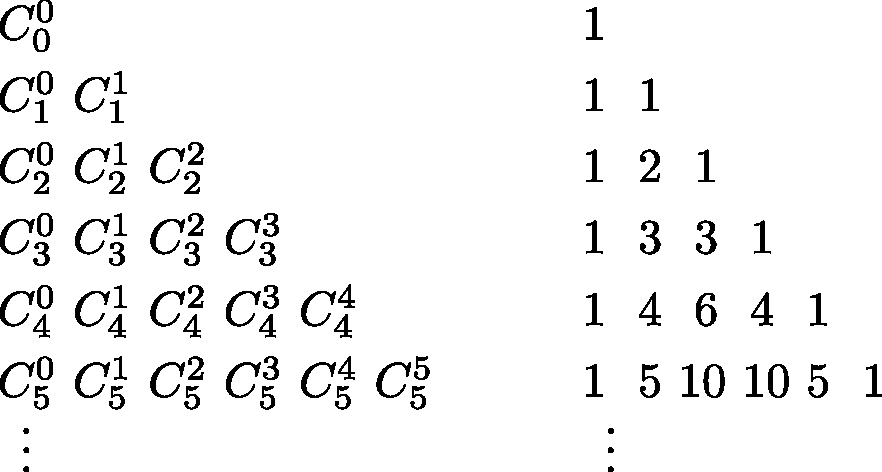
\includegraphics[width=\linewidth]{images/triangulopascal}
\end{image}%
\tcblower
\end{figureptx}%
\end{definition}
\begin{theorem}{}{}{g:theorem:idp217}%
\terminology{(Relação de Stifel)}%
\begin{equation*}
C_n^p + C_n^{p+1} = C_{n+1}^{p+1}. 
\end{equation*}
\end{theorem}
\begin{proof}{}{g:proof:idp218}
%
\begin{align*}
C_n^p + C_n^{p+1}= \amp ~\frac{n!}{p!\times (n-p)!} + \frac{n!}{(p+1)!\times (n-p-1)!}   \\
= \amp ~ \frac{(p+1)\times n!}{(p+1)\times p!\times (n-p)!} + \frac{(n-p)\times n!}{(n-p)\times(p+1)!\times (n-p-1)!}  \\
= \amp ~ \frac{n!\times((p+1)+(n-p)) }{(n-p)!\times(p+1)!}  \\
= \amp ~ \frac{n!\times(n+1) }{(n-p)!\times(p+1)!}  \\
= \amp ~ \frac{(n+1)!}{(p+1)!\times (n-p)!}  \\
= \amp ~ C_{n+1}^{p+1}  \qedhere
\end{align*}
\end{proof}
\begin{theorem}{}{}{g:theorem:idp219}%
\terminology{(Relação das Combinações Complementares)}%
\begin{equation*}
C_n^p = C_n^{n-p}.
\end{equation*}
\end{theorem}
\begin{proof}{}{g:proof:idp220}
%
\begin{equation*}
C_n^p= \frac{n!}{p!\times (n-p)!} = \frac{n!}{(n-p)!\times p!} = C_n^{n-p}.\qedhere
\end{equation*}
\end{proof}
\begin{theorem}{}{}{g:theorem:idp221}%
\terminology{(Teorema das Linhas)}%
\begin{equation*}
C_n^0 + C_n^1 +C_n^2 + \cdots + C_n^n = 2^n.
\end{equation*}
\end{theorem}
\begin{proof}{}{g:proof:idp222}
Observe que%
%
\begin{equation*}
C_n^i \text{ é número de subconjuntos com}~ i ~\text{elementos, de } \{1, 2, \ldots, n\}. 
\end{equation*}
Ou seja, a soma%
\begin{equation*}
C_n^0 + C_n^1 +C_n^2 + \cdots + C_n^n
\end{equation*}
conta o número de todos os subconjuntos, de um conjunto com n elementos.%
\par
Essa quantidade é \(2^n\), pois para formar um subconjunto, deve-se decidir, para cada elemento do conjunto, se ele pertencerá ou não ao subconjunto. Há dois modos de decidir o que fazer com o primeiro elemento do conjunto, 2 modos com o segundo e assim por diante. Portanto o valor da soma de uma linha do Triângulo de Pascal é%
\begin{equation*}
2^n. \qedhere
\end{equation*}
%
\end{proof}
\begin{fact}{}{}{g:fact:idp223}%
Qual o valor da soma%
\begin{equation*}
S = \frac{1}{2}C_n^1 + \frac{1}{3}C_n^2 + \cdots + \frac{1}{n+1}C_n^n? 
\end{equation*}
%
\textbf{\blocktitlefont Solução}.\quad{}%
\begin{align*}
S = \amp \sum_{k=1}^n \frac{1}{k+1}C_n^k  \\
= \amp \sum_{k=1}^n \frac{1}{k+1}\cdot \frac{n!}{k!(n-k)!}  \\
= \amp \sum_{k=1}^n \frac{1}{k+1}\cdot \frac{n!}{k!(n-k)!}\cdot \frac{n+1}{n+1}  \\
= \amp \frac{1}{n+1}\sum_{k=1}^n \frac{(n+1)!}{(k+1)!(n-k)!}  \\
= \amp \frac{1}{n+1}\sum_{k=1}^n C_{n+1}^{k+1}  \\
= \amp \frac{1}{n+1}\left( -C_{n+1}^0 - C_{n+1}^1 +\underbrace{C_{n+1}^0 + C_{n+1}^1 + \cdots+C_{n+1}^{n+1}}_{=2^{n+1}} \right)  \\
= \amp \frac{1}{n+1}\left( 2^{n+1} - n -2 \right).  
\end{align*}
\end{fact}
\begin{theorem}{}{}{g:theorem:idp224}%
\terminology{(Teorema das Colunas)}%
\begin{equation*}
C_p^p + C_{p+1}^p + C_{p+2}^p + \cdots + C_{p+n}^p = C_{p+n+1}^{p+1}.
\end{equation*}
\end{theorem}
\begin{proof}{}{g:proof:idp225}
Vamos aplicar a relação de Stifel aos elementos da coluna \(p+1\):%
\begin{align*}
C_{p+1}^{p+1} = \amp C_p^{p+1} + C_p^p  \\
C_{p+2}^{p+1} = \amp C_{p+1}^{p+1} + C_{p+1}^p  \\
C_{p+3}^{p+1} = \amp C_{p+2}^{p+1} + C_{p+2}^p   \\
\vdots ~~~ = \amp ~~~~~~ \vdots   \\
C_{p+n}^{p+1} = \amp C_{p+n-1}^{p+1} + C_{p+n-1}^p  \\
C_{p+n+1}^{p+1} = \amp C_{p+n}^{p+1} + C_{p+n}^p  
\end{align*}
Somando tudo, ficamos com%
\begin{equation*}
C_{p+n+1}^{p+1} = C_p^{p+1} + C_p^p + C_{p+1}^p + C_{p+2}^p +\cdots + C_{p+n-1}^p + C_{p+n}^p.
\end{equation*}
Como \(C_p^{p+1} = 0\), obtemos o resultado:%
\begin{equation*}
C_{p+n+1}^{p+1} = C_p^p + C_{p+1}^p + C_{p+2}^p +\cdots + C_{p+n-1}^p + C_{p+n}^p.\qedhere
\end{equation*}
\end{proof}
\begin{fact}{}{}{g:fact:idp226}%
Qual o valor da soma%
\begin{equation*}
S = 1^2\cdot2 + 2^2\cdot3+  3^2\cdot4+\cdots+n^2\cdot(n+1)? 
\end{equation*}
%
\textbf{\blocktitlefont Solução}.\quad{}Note que%
\begin{align*}
S = \amp \sum_{k=1}^{n} k^2\cdot (k+1)  \\
= \amp \sum_{k=1}^{n} k^3+k^2  
\end{align*}
Para usarmos o Teorema das Colunas, precisamos que no somatório apareca um produto de números consecutivos, pois%
\begin{equation*}
k\cdot(k+1)\cdot(k+2) = 3!\frac{(k+2)!}{3!(k-1)!} = 3!\cdot C_{k+2}^{3}.
\end{equation*}
Então, vamos procurar valores para \(A, B, C\) e \(D\), para os quais, vale a igualdade%
\begin{align*}
k^3+k^2 = \amp ~ Ak(k+1)(k+2) + Bk(k+1) + Ck +D  \\
= \amp ~ k^3(A) + k^2(3A+B) + k(2A+B+C) +D  
\end{align*}
igualando os coeficientes, obtemos%
\begin{equation*}
\begin{cases} 
A = ~ 1 \\
3A+B  = ~ 1 \\
2A+B+C  = ~ 0 \\
D = ~ 0 \\
\end{cases}
\end{equation*}
Portanto,  \(A= 1\) e  \(B = -2\). Agora podemos terminar o cálculo da soma%
\begin{align*}
S = \amp ~ \sum_{k=1}^{n} k^3+k^2  \\
= \amp ~ \sum_{k=1}^{n} k(k+1)(k+2) - 2 \sum_{k=1}^{n} k(k+1)  \\
= \amp ~ 3!\sum_{k=1}^{n} C_{k+2}^3 - 2\cdot 2! \sum_{k=1}^{n} C_{k+1}^2  \\
= \amp ~ 6C_{n+3}^4 - 4C_{n+2}^3  \\
= \amp ~ \frac{3n^4+10n^3+9n^2+2n}{12}.  
\end{align*}
\end{fact}
\begin{theorem}{}{}{g:theorem:idp227}%
\terminology{(Teorema das Diagonais)}%
\begin{equation*}
C_n^0 + C_{n+1}^1 + C_{n+2}^2 + \cdots + C_{n+p}^p = C_{n+p+1}^p
\end{equation*}
\end{theorem}
\begin{proof}{}{g:proof:idp228}
Aplicando o Teorema 2 (Relação das Combinações Complementares), em cada \(C_{n+i}^i\) obtemos%
\begin{equation*}
C_n^0 + C_{n+1}^1 + C_{n+2}^2 + \cdots + C_{n+p}^p = \underbrace{C_{n}^n+C_{n+1}^n+C_{n+2}^n+\cdots+C_{n+p}^n}_{(*)}. 
\end{equation*}
Aplicando o Teorema 4 (Teorema das Colunas), no lado direito da igualdade anterior, obtemos%
\begin{equation*}
\overbrace{C_{n}^n+C_{n+1}^n+C_{n+2}^n+\cdots+C_{n+p}^n}^{(*)} = \underbrace{C_{n+p+1}^{n+1}}_{(**)}.
\end{equation*}
Aplicando novamente o Teorema 2, obtemos%
\begin{equation*}
\overbrace{C_{n+p+1}^{n+1}}^{(**)} =  C_{n+p+1}^{p}. 
\end{equation*}
O que mostra o resultado.%
\end{proof}
\begin{theorem}{}{}{g:theorem:idp229}%
%
\begin{equation*}
\text{a) Se } p\lt \frac{n-1}{2}, \text{ então }  C_n^p\lt C_n^{p+1}. 
\end{equation*}
%
\begin{equation*}
\text{b) Se } p> \frac{n-1}{2}, \text{ então }  C_n^p>C_n^{p+1}. 
\end{equation*}
\end{theorem}
\begin{proof}{}{g:proof:idp230}
Vamos analisar a diferença \(C_n^{p+1}-C_n^p\):%
\begin{align*}
C_n^{p+1}-C_n^p = \amp ~ \frac{n!}{(p+1)!(n-p-1)!} - \frac{n!}{p!(n-p)!}  \\
= \amp ~ \frac{n!}{(p+1) p!(n-p-1)!} - \frac{n!}{p!(n-p)(n-p-1)!}  \\
= \amp ~ \frac{n!(n-p) - n!(p+1)}{(p+1)!(n-p)!}  \\
= \amp ~ \frac{n!(n-2p-1))}{(p+1)! (n-p)!}  
\end{align*}
Oberve que \(n!, (p+1)!\) e \((n-p)!\) são positivos, portanto o sinal de \(C_n^{p+1}-C_n^p\), será determinado pelo sinal de%
\begin{equation*}
n-2p-1.
\end{equation*}
Logo,%
\begin{equation*}
\text{Se } n-2p-1>0, \text{ então } p\lt\frac{n-1}{2} \Rightarrow C_n^{p+1}-C_n^{p}>0 \Rightarrow C_n^{p}\lt C_n^{p+1}. 
\end{equation*}
%
\begin{equation*}
\text{Se } n-2p-1\lt 0, \text{ então } p>\frac{n-1}{2} \Rightarrow C_n^{p+1}-C_n^{p}\lt 0 \Rightarrow C_n^{p}>C_n^{p+1}.   \qedhere
\end{equation*}
%
\end{proof}
%
%
\typeout{************************************************}
\typeout{Exercícios 4.1.1 Exercícios}
\typeout{************************************************}
%
\begin{exercises-subsection}{Exercícios}{}{Exercícios}{}{}{g:exercises:idp231}
\begin{divisionexercise}{1}{}{}{g:exercise:idp232}%
Tem-se \(n\) comprimidos de substâncias distintas, solúveis em água e incapazes de reagir entre si. Quantas soluções distintas podem ser obtidas dissolven-se um ou mais desses comprimidos em um copo com água?%
\par\smallskip%
\noindent\textbf{\blocktitlefont Resposta}.\hypertarget{g:answer:idp233}{}\quad{}\(2^n-1\)%
\end{divisionexercise}%
\begin{divisionexercise}{2}{}{}{g:exercise:idp234}%
Calcule o valor da soma%
\begin{equation*}
S = 20\cdot21 + 21\cdot 22 +\cdots + 130\cdot 131.
\end{equation*}
%
\par\smallskip%
\noindent\textbf{\blocktitlefont Resposta}.\hypertarget{g:answer:idp235}{}\quad{}746660%
\end{divisionexercise}%
\begin{divisionexercise}{3}{}{}{g:exercise:idp236}%
Calcule o valor de%
\begin{equation*}
S = \sum_{k=1}^{n}k(3k+1).
\end{equation*}
%
\par\smallskip%
\noindent\textbf{\blocktitlefont Resposta}.\hypertarget{g:answer:idp237}{}\quad{}\(n^{3} + 2 \, n^{2} + n\)%
\end{divisionexercise}%
\begin{divisionexercise}{4}{}{}{g:exercise:idp238}%
Calcule%
\begin{equation*}
CR_n^0 + CR_n^1+\cdots+ CR_n^p.
\end{equation*}
%
\par\smallskip%
\noindent\textbf{\blocktitlefont Resposta}.\hypertarget{g:answer:idp239}{}\quad{}\(C_{n+p}^p\)%
\end{divisionexercise}%
\end{exercises-subsection}
\end{sectionptx}
%
%
\typeout{************************************************}
\typeout{Seção 4.2 Binômio de Newton}
\typeout{************************************************}
%
\begin{sectionptx}{Binômio de Newton}{}{Binômio de Newton}{}{}{x:section:section-binomio-newton}
\begin{objectives}{Objetivos}{x:objectives:objetivos-binomio-newton}
%
\begin{enumerate}
\item{}Enunciar e demonstrar o Teorema do Binômio de Newton%
\item{}Exemplificar.%
\item{}Resolver exemplos no Sage.%
\end{enumerate}
\end{objectives}
\begin{theorem}{}{}{g:theorem:idp240}%
Se \(x\) e \(a\) são número reais e \(n\) é um inteiro positivo,%
\begin{equation*}
(x+a)^n  = \sum_{k=0}^n C_n^k x^ka^{n-k}.
\end{equation*}
%
\end{theorem}
\begin{proof}{}{g:proof:idp241}
Observe que%
\begin{equation*}
(x+a)^n  = \overbrace{(x+a)(x+a)\cdots(x+a)}^{n \text{ parcelas}}.
\end{equation*}
Cada termo, do desenvolvimento, é obtido escolhendo-se em cada parênteses um, \(x\) ou um \(a\) e multiplicando-se os escolhidos.%
\par
Para cada valor de \(k, 0\leq k \leq n\), se escolhermos \(x\) em \(k\) dos parênteses, \(a\) será escolhido em \(n-k\) dos parênteses e o produto será igual a \(x^ka^{n-k}\). Isto pode ser feito de \(C_n^k\) modos. Então \((x-a)^n\) é uma soma na qual, para cada \(k\in\{0, 1, \ldots, n\}\), existem \(C_n^k\) parcelas iguais a \(x^ka^{n-k}\). Portanto%
\begin{equation*}
(x+a)^n  = \sum_{k=0}^n C_n^k x^ka^{n-k}.\qedhere
\end{equation*}
%
\end{proof}
\begin{remark}{}{g:remark:idp242}%
Destacamos o termo geral e o fato de que o desenvolvimento do Binômio de Newton pode ser desenvolvido na ordem inversa:%
\par
1)%
\begin{equation*}
(x+a)^n   = \underbrace{C_n^0x^0a^{n-0}}_{\text{1º termo: } T_1} + \underbrace{C_n^1x^1a^{n-1}}_{\text{2º termo: } T_2} + \underbrace{C_n^2x^2a^{n-2}}_{\text{3º termo: } T_3} + \cdots + \underbrace{C_n^nx^na^{n-n}}_{\text{(n+1)º termo: } T_{n+1}}.
\end{equation*}
O \(k\)-ésimo termo \((k=1, \ldots, n+1)\) do desenvolvimento é dado por:%
\begin{equation*}
T_{k} = C_n^{k-1}x^{k-1}a^{n-k+1}. 
\end{equation*}
2) Observe também que:%
\begin{equation*}
(x+a)^n = (a+x)^n.
\end{equation*}
Portanto%
\begin{equation*}
(x+a)^n = (a+x)^n =  C_n^0a^0x^n+C_n^1a^1x^{n-1}+ C_n^2a^2x^{n-2}+\cdots + C_n^na^nx^0.
\end{equation*}
%
\end{remark}
\begin{fact}{}{}{g:fact:idp243}%
Considere o binômio de Newton%
\begin{equation*}
\left(x^4-\frac{1}{x^2}\right)^{11}.
\end{equation*}
Determine os coeficientes de a) \(x^2\) no desenvolvimento do binômio;%
 \par
b) \(x^5\) no desenvolvimento do binômio;%
 \par
c) \(x^8\) no desenvolvimento do binômio.%
%
\textbf{\blocktitlefont Solução}.\quad{}O \(k\)-ésimo termo do desenvolvimento é%
\begin{align*}
T_k = \amp ~ C_{11}^{k-1}(x^4)^{k-1}\left(-\frac{1}{x^2}\right)^{11-k+1}  \\
= \amp ~ (-1)^{12-k}C_{11}^{k-1}x^{4(k-1)}x^{-2(12-k)}  \\
= \amp ~ (-1)^{12-k}C_{11}^{k-1}x^{6k-28}  
\end{align*}
%
\par
\terminology{item a)} Para que \(6k-28 = 2\), temos \(k=5\), logo estamos procurando o 5º termo:%
\begin{equation*}
T_5 = (-1)^{7}C_{11}^4x^2.
\end{equation*}
E portanto o coeficiente é \((-1)^{7}C_{11}^4 = -330\).%
\par
\terminology{item b)} \(6k-28 = 5\) não possui solução em \(\mathbb{Z}\), portanto o coeficiente de \(x^5\) é zero.%
\par
\terminology{item c)}Para que \(6k-28 = 8\), temos \(k=6\), logo estamos procurando o 6º termo:%
\begin{equation*}
T_6 = (-1)^{6}C_{11}^5x^8.
\end{equation*}
E portanto o coeficiente é \((-1)^{6}C_{11}^5 = 462\).%
\end{fact}
\begin{technology}{}{g:technology:idp244}%
No Sage, podemos obter a expanção do polinômio da seguinte forma:%
\begin{sageinput}
((x^4 - 1/x^2)^11).expand()
\end{sageinput}
\begin{sageoutput}
x^44 - 11*x^38 + 55*x^32 - 165*x^26 + 330*x^20 - 462*x^14 + 462*x^8 - 330*x^2 + 165/x^4 - 55/x^10 + 11/x^16 - 1/x^22
\end{sageoutput}
Os coeficientes do polinômio, podem ser obtidos da seguinte forma:%
\begin{sageinput}
((x^4 - 1/x^2)^11).coefficients()
\end{sageinput}
\begin{sageoutput}
[[-1, -22],
 [11, -16],
 [-55, -10],
 [165, -4],
 [-330, 2],
 [462, 8],
 [-462, 14],
 [330, 20],
 [-165, 26],
 [55, 32],
 [-11, 38],
 [1, 44]]
\end{sageoutput}
\end{technology}
\begin{fact}{}{}{g:fact:idp245}%
Determine o termo máximo do desenvolvimento de%
\begin{equation*}
\left(1 + \frac{1}{4}\right)^{10}.
\end{equation*}
%
\textbf{\blocktitlefont Solução}.\quad{}Como%
\begin{equation*}
\left(1 + \frac{1}{4}\right)^{10} = \frac{1}{1024} + \frac{5}{256} + \frac{5}{32} + \frac{5}{8} + \frac{5}{4}+ 1.
\end{equation*}
O termo máximo é%
\begin{equation*}
\frac{5}{4}.
\end{equation*}
%
\end{fact}
\begin{fact}{}{}{g:fact:idp246}%
Determine o termo máximo do desenvolvimento de%
\begin{equation*}
\left(1 + \frac{1}{4}\right)^{70}.
\end{equation*}
%
\textbf{\blocktitlefont Solução}.\quad{}O \(k\)-ésimo termo é%
\begin{equation*}
T_{k} = C_{70}^{k-1}1^{k-1}\left(\frac{1}{4}\right)^{71-k} = C_{70}^{k-1}\cdot\frac{1}{4^{71-k}}\text{.}
\end{equation*}
\(T_{k+1}> T_{k}\) se%
\begin{equation*}
C_{70}^{k}\cdot\frac{1}{4^{70-k}} > C_{70}^{k-1}\cdot\frac{1}{4^{71-k}} 
\end{equation*}
Isto é%
\begin{equation*}
\frac{70!}{k!(70-k)!}\cdot\frac{1}{4^{70-k}} > \frac{70!}{(k-1)!(71-k)!}\cdot\frac{1}{4^{71-k}}, 
\end{equation*}
ou seja,%
\begin{equation*}
\frac{(71-k)!}{(70-k)!} > \frac{k!}{(k-1)!}\cdot\frac{4^{70-k}}{4^{71-k}}, 
\end{equation*}
e simplificando temos%
\begin{equation*}
\frac{(71-k)}{1} > \frac{k}{1}\cdot\frac{1}{4}. 
\end{equation*}
Portanto, \(71-k > k/4 \), logo \(k\lt 56, 8\).%
\par
Assim, temos  \(T_{k} \lt  T_{k+1}\) para \(k = 1, 2, \ldots, 56\) e portanto o maior termo é:%
\begin{equation*}
T_{57} = C_{70}^{56}\cdot\frac{1}{4^{14}} = \frac{24156719613645}{33554432}.
\end{equation*}
%
\end{fact}
\begin{technology}{Faça você mesmo.}{g:technology:idp247}%
\begin{figureptx}{Os termos máximo e mínimo.}{x:figure:interactive-binomio}{}%
\centering
O termo máximo do desenvolvimento de%
\begin{equation*}
\left(1 + \frac{1}{4}\right)^{70}.
\end{equation*}
Troque os valores de \(x\), \(a\) e \(n\), para obter o termo máximo e o termo mínimo do desenvolvimento de%
\begin{equation*}
(x+a)^n.
\end{equation*}
%
\setlength{\qrsize}{9em}
\setlength{\previewwidth}{\linewidth}
\addtolength{\previewwidth}{-\qrsize}
\begin{tcbraster}[raster columns=2, raster column skip=1pt, raster halign=center, raster force size=false, raster left skip=0pt, raster right skip=0pt]%
\begin{tcolorbox}[previewstyle, width=\previewwidth]%
\IfFileExists{images/interactive-binomio-preview.png}%
{\includegraphics[width=0.80\linewidth,height=\qrsize,keepaspectratio]{images/interactive-binomio-preview.png}}%
{\small{}Specify static image with \mono{@preview} attribute,\\Or create and provide automatic screenshot as \mono{images/interactive-binomio-preview.png} via the \mono{mbx} script}%
\end{tcolorbox}%
\begin{tcolorbox}[qrstyle]%
{\hypersetup{urlcolor=black}\qrcode[height=\qrsize]{/interactive-binomio.html}}%
\end{tcolorbox}%
\end{tcbraster}%
\tcblower
\end{figureptx}%
\end{technology}
\begin{fact}{}{}{g:fact:idp248}%
Qual é a soma dos coeficientes do desenvolvimento de%
\begin{equation*}
(5x^{11} - 6x^{4})^{25}. 
\end{equation*}
%
\textbf{\blocktitlefont Solução}.\quad{}Seja \(p(x) = a_0 + a_1x + a_2x^2 + \cdots + a_nx^n\), a soma dos coeficientes de \(p(x)\) é igual a%
\begin{equation*}
p(1) = a_0 + a_1(1) + a_2(1)^2 + \cdots + a_n(1)^n.
\end{equation*}
Portando a soma dos coeficientes do desenvolvimento de \(q(x) = (5x^{11} - 6x^{4})^{25}\) é%
\begin{equation*}
q(1) = (5 - 6)^{25} = -1.
\end{equation*}
%
\end{fact}
\begin{theorem}{}{}{g:theorem:idp249}%
%
\begin{equation*}
T_{k+1} = \frac{n-k+1}{k}\cdot\frac{x}{a}\cdot T_k
\end{equation*}
%
\end{theorem}
\begin{proof}{}{g:proof:idp250}
%
\begin{equation*}
T_{k+1} = C_n^kx^ka^{n-k} = \frac{n-k+1}{k}C_n^{k-1}x^ka^{n-k} 
\end{equation*}
e%
\begin{equation*}
T_{k} = C_n^{k-1}x^{k-1}a^{n-k+1}. 
\end{equation*}
Portanto,%
\begin{equation*}
T_{k+1} = \frac{n-k+1}{k}\cdot\frac{x}{a}\cdot T_k.\qedhere
\end{equation*}
%
\end{proof}
%
%
\typeout{************************************************}
\typeout{Exercícios 4.2.1 Exercícios}
\typeout{************************************************}
%
\begin{exercises-subsection}{Exercícios}{}{Exercícios}{}{}{g:exercises:idp251}
\begin{divisionexercise}{1}{}{}{g:exercise:idp252}%
Determine o coeficiente de \(x^5\) no desenvolvimento de%
\begin{equation*}
\left( x^3 - \frac{1}{x^2} \right)^{15}.
\end{equation*}
%
\par\smallskip%
\noindent\textbf{\blocktitlefont Resposta}.\hypertarget{g:answer:idp253}{}\quad{}6435%
\end{divisionexercise}%
\begin{divisionexercise}{2}{}{}{g:exercise:idp254}%
Determine o coeficiente de \(x^{50}\) no desenvolvimento de%
\begin{equation*}
(x^2+3)^{10}(x^3-3)^{11}.
\end{equation*}
%
\par\smallskip%
\noindent\textbf{\blocktitlefont Resposta}.\hypertarget{g:answer:idp255}{}\quad{}-33%
\end{divisionexercise}%
\begin{divisionexercise}{3}{}{}{g:exercise:idp256}%
Calcule o termo máximo do desenvolvimento de%
\begin{equation*}
\left(1+\frac{1}{5}\right)^{50}.
\end{equation*}
%
\par\smallskip%
\noindent\textbf{\blocktitlefont Resposta}.\hypertarget{g:answer:idp257}{}\quad{}\(T_{43} = C_{50}^{42}\left(\dfrac{1}{5}\right)^{8} = \dfrac{21475146}{15625}\)%
\end{divisionexercise}%
\begin{divisionexercise}{4}{}{}{g:exercise:idp258}%
Qual é o maior dos números%
%
\begin{equation*}
a = 151^{60} \text{ e } b = 150^{60} + 149^{60}? 
\end{equation*}
\par\smallskip%
\noindent\textbf{\blocktitlefont Resposta}.\hypertarget{g:answer:idp259}{}\quad{}b%
\end{divisionexercise}%
\end{exercises-subsection}
\end{sectionptx}
%
%
\typeout{************************************************}
\typeout{Seção 4.3 Polinômio de Leibniz}
\typeout{************************************************}
%
\begin{sectionptx}{Polinômio de Leibniz}{}{Polinômio de Leibniz}{}{}{x:section:section-polinomio-leibniz}
\begin{objectives}{Objetivos}{x:objectives:objetivos-polinomio-leibniz}
%
\begin{enumerate}
\item{}Enunciar e demonstrar o Teorema do Polinômio de Leibniz%
\item{}Exemplificar.%
\item{}Resolver um exemplo no Sage.%
\end{enumerate}
\end{objectives}
\begin{theorem}{}{}{g:theorem:idp260}%
%
\begin{equation*}
(x_1+x_2+\cdots + x_p)^n   = \sum_{\alpha_1 + \alpha_2 +\cdots + \alpha_p = n} \frac{n!}{\alpha_1!\alpha_2!\cdots\alpha_p!}x_1^{\alpha_1}x_2^{\alpha_2}\cdots x_p^{\alpha_p}\\
\end{equation*}
Na qual, para cada \(i\in\{1, 2, \ldots, p\}\), \(\alpha_i\in \{j ~|~ j\in \mathbb{Z}\geq 0\}\), ou seja \(\alpha_i\) é um inteiro não negativo.%
\end{theorem}
\begin{proof}{}{g:proof:idp261}
Temos%
\begin{equation*}
(x_1+x_2+\cdots + x_p)^n  = (x_1+x_2++\cdots + x_p)\cdots(x_1+x_2++\cdots + x_p)
\end{equation*}
Um termo genérico do produto é obtido escolhendo um \(x_i\) em cada parênteses e multiplicando os escolhidos. Se em \(\alpha_1\) dos parênteses escolhermos \(x_1\), em \(\alpha_2\) dos parênteses escolhermos \(x_2\), \(\ldots\), obteremos%
\begin{equation*}
x_1^{\alpha_1}x_2^{\alpha_2}\cdots x_p^{\alpha_p}, \text{ satisfazendo } \alpha_1 + \alpha_2 +\cdots + \alpha_p = n. 
\end{equation*}
Agora falta responder quantas vezes o termo \(x_1^{\alpha_1}x_2^{\alpha_2}\cdots x_p^{\alpha_p}\) aparece no desenvolvimento.%
\par
O termo \(x_1^{\alpha_1}x_2^{\alpha_2}\cdots x_p^{\alpha_p}\) aparece tantas vezes, quantas são as formas de escolher, nos \(n\) parênteses, \(\alpha_1\) deles para escolher o \(x_1\), \(\alpha_2\) deles para escolher o \(x_2\), \(\ldots\). Isto pode ser feito de%
\begin{equation*}
C_n^{\alpha_1}\cdot C_{n-\alpha_1}^{\alpha_2}\cdots C_{n-\alpha_1-\alpha_2-\cdots -\alpha_{p-1}}^{\alpha_p} = \frac{n!}{\alpha_1!\alpha_2!\cdots\alpha_p!} 
\end{equation*}
maneiras, o que mostra o resultado.%
\end{proof}
\begin{fact}{}{}{g:fact:idp262}%
Considere o polinômio:%
\begin{equation*}
(x^3-x+5)^8 
\end{equation*}
Determine os coeficientes de a) \(x^2\) no desenvolvimento;%
 \par
b) \(x^4\) no desenvolvimento.%
%
\textbf{\blocktitlefont Solução}.\quad{}%
\begin{equation*}
(x^3-x+5)^8   = \sum_{\alpha_1 + \alpha_2 + \alpha_3 = 8} \frac{8!}{\alpha_1!\alpha_2!\alpha_3!}(x^3)^{\alpha_1}(-x)^{\alpha_2}5^{\alpha_3}\\
\end{equation*}
%
\par
\terminology{item a)} Para que o expoente de \(x\) seja 2, devemos ter \(x^{3\alpha_1}x^{\alpha_2} = x^2\), juntando com a condição \(\alpha_1+\alpha_2+\alpha_3 = 8\), temos%
\begin{equation*}
\begin{cases} 
\alpha_1 + \alpha_2 +\alpha_3    =  8 \\
~~~~ ~~~~ 3\alpha_1 + \alpha_2  =  2 \end{cases}
\end{equation*}
Assim, \(\alpha_1 = 0, \alpha_2 = 2\) e \(\alpha_3 = 6.\) E a soma dos termos que possuem \(x^2\) é:%
\begin{equation*}
\frac{8!}{0!\times 2! \times 6!} 5^6x^2 = 437500x^2.
\end{equation*}
%
\par
\terminology{item b)} Para que o expoente de \(x\) seja 4, devemos ter \(x^{3\alpha_1}x^{\alpha_2} = x^4\), juntando com a condição \(\alpha_1+\alpha_2+\alpha_3 = 8\), temos%
\begin{equation*}
\begin{cases} 
\alpha_1 + \alpha_2 +\alpha_3    =  8 \\
~~~~ ~~~~ 3\alpha_1 + \alpha_2  =  4 \end{cases}
\end{equation*}
Temos duas soluções:%
\begin{equation*}
\begin{cases} 
\alpha_1 = 0, \alpha_2 = 4 \text{ e }\alpha_3 = 4 \\
\alpha_1 = 1, \alpha_2 = 1 \text{ e } \alpha_3 = 6 \end{cases}
\end{equation*}
E a soma dos termos que possuem \(x^4\) é:%
\begin{equation*}
\frac{8!}{0!\times 4! \times 4!} 5^4x^2 - \frac{8!}{1!\times 1! \times 6!} 5^6x^2 = -831250x^2.
\end{equation*}
%
\end{fact}
\begin{technology}{}{g:technology:idp263}%
No Sage, podemos obter a expanção do polinômio da seguinte forma:%
\begin{sageinput}
((x^3-x+5)^8).expand()
\end{sageinput}
\begin{sageoutput}
x^24 - 8*x^22 + 40*x^21 + 28*x^20 - 280*x^19 + 644*x^18 + 840*x^17 - 4130*x^16 + 5600*x^15 + 10444*x^14 - 33600*x^13 + 29778*x^12 + 69160*x^11 - 164508*x^10 + 105280*x^9 + 258301*x^8 - 490040*x^7 + 263200*x^6 + 518000*x^5 - 831250*x^4 + 450000*x^3 + 437500*x^2 - 625000*x + 390625
\end{sageoutput}
Os coeficientes do polinômio, podem ser obtidos da seguinte forma:%
\begin{sageinput}
((x^3-x+5)^8).coefficients()
\end{sageinput}
\begin{sageoutput}
[[390625, 0],
 [-625000, 1],
 [437500, 2],
 [450000, 3],
 [-831250, 4],
 [518000, 5],
 [263200, 6],
 [-490040, 7],
 [258301, 8],
 [105280, 9],
 [-164508, 10],
 [69160, 11],
 [29778, 12],
 [-33600, 13],
 [10444, 14],
 [5600, 15],
 [-4130, 16],
 [840, 17],
 [644, 18],
 [-280, 19],
 [28, 20],
 [40, 21],
 [-8, 22],
 [1, 24]]
\end{sageoutput}
\end{technology}
%
%
\typeout{************************************************}
\typeout{Exercícios 4.3.1 Exercícios}
\typeout{************************************************}
%
\begin{exercises-subsection}{Exercícios}{}{Exercícios}{}{}{g:exercises:idp264}
\begin{divisionexercise}{1}{}{}{g:exercise:idp265}%
Determine o coeficiente de \(x^{12}\) no desenvolvimento de%
%
\begin{equation*}
\left( 1+x^4+x^8 \right)^{12}.
\end{equation*}
\par\smallskip%
\noindent\textbf{\blocktitlefont Resposta}.\hypertarget{g:answer:idp266}{}\quad{}336%
\end{divisionexercise}%
\end{exercises-subsection}
\end{sectionptx}
\end{chapterptx}
%
%
\typeout{************************************************}
\typeout{Capítulo 5 Probabilidade}
\typeout{************************************************}
%
\begin{chapterptx}{Probabilidade}{}{Probabilidade}{}{}{x:chapter:probabilidade}
\begin{introduction}{}%
Neste capítulo é abordado ....%
\end{introduction}%
%
%
\typeout{************************************************}
\typeout{Seção 5.1 Espaços de Probabilidade}
\typeout{************************************************}
%
\begin{sectionptx}{Espaços de Probabilidade}{}{Espaços de Probabilidade}{}{}{x:section:section-espacos-probabilidade}
\begin{objectives}{Objetivos}{x:objectives:objetivos-espacos-probabilidade}
%
\begin{enumerate}
\item{}Definir Espaço Amostral e Evento.%
\item{}Definir Probabilidade.%
\item{}Demonstrar um teorema com propriedades de probabilidade.%
\item{}Exemplificar.%
\end{enumerate}
\end{objectives}
\begin{definition}{}{g:definition:idp267}%
Chamaremos de \emph{espaço amostral} o conjunto de todos os resultados possíveis de uma experiência aleatória. Denotaremos o espaço amostral por \(\Omega\) e só vamos considerar o caso de \(\Omega\) ser finito.%
\par
Os subconjuntos de \(\Omega\) serão chamados de \emph{eventos}. Diremos que um evento ocorre quando o resultado da experiência pertence ao evento.%
\end{definition}
\begin{definition}{}{x:definition:def-probabilidade}%
Seja \(\Omega\) um espaço amostral. Uma probabilidade sobre \(\Omega\) é uma função que associa a cada evento \(A\subset\Omega\) um número \(P(A)\) de forma que:%
\begin{align*}
a) \amp ~ \text{Para todo evento }A ,~~ 0\leq P(A)\leq 1;  \\
b) \amp ~ P(\Omega)=1;  \\
c) \amp ~ \text{Se } A\cap B = \emptyset \text{ então } P(A\cup B) = P(A) + P(B).  
\end{align*}
%
\end{definition}
\begin{fact}{}{}{g:fact:idp268}%
Ao lançar uma moeda observe a face que cai voltada para cima.%
\par
O espaço amostral é \(\Omega = \{\text{Cara}, \text{Coroa}\},\) os eventos são%
\begin{equation*}
\emptyset, ~~ A = \{\text{Cara}\}, ~~B = \{\text{Coroa}\} ~~\text{ e }~~ \Omega. 
\end{equation*}
a) Vamos definir uma probabilidade para \(\Omega\), que chamaremos de \(P_1\):%
\begin{equation*}
P_1(\emptyset)=0, ~~ P_1(A) = \frac{1}{2}, ~~P_1(B) = \frac{1}{2} ~~\text{ e }~~ P_1(\Omega)=1.
\end{equation*}
b) Vamos definir outra probabilidade para \(\Omega\), que chamaremos de \(P_2\):%
\begin{equation*}
P_2(\emptyset)=0, ~~ P_2(A) = \frac{1}{10}, ~~P_2(B) = \frac{9}{10} ~~\text{ e }~~ P_2(\Omega)=1.
\end{equation*}
Observe que \(P_1\) e \(P_2\) satisfazem a definição de probabilidade.%
\end{fact}
\begin{fact}{}{}{g:fact:idp269}%
Um modelo de probabilidade muito utilizado é o equiprobabilístico, que é o caso de \(P_1\) do exemplo anterior.%
\par
O caso geral deste modelo, ou seja para \(\#\Omega = n\), atribuímos a cada evento unitário a probabilidade%
\begin{equation*}
\frac{1}{n}. 
\end{equation*}
Pois, se \(\Omega = \{e_1, e_2, \ldots, e_n\}\) e \(P(\{e_1\}) = P(\{e_2\}) = \cdots = P(\{e_n\})= k\). Pelo item c) da \hyperref[x:definition:def-probabilidade]{Definição~{\xreffont\ref{x:definition:def-probabilidade}}}, temos%
\begin{align*}
1 = \amp ~P(\Omega) = P(\{e_1, e_2, \ldots, e_n\}) = P(\{e_1\} \cup \{e_2\}\cup \ldots\cup \{e_n\})   \\
= \amp ~P(\{e_1\}) \cup P(\{e_2\})\cup \ldots\cup P(\{e_n\}) \\
= \amp ~ \underbrace{k+k+\cdots+k}_{\text{n termos}} = nk  
\end{align*}
Portanto,%
\begin{equation*}
k = \frac{1}{n}. 
\end{equation*}
%
\end{fact}
\begin{fact}{}{}{g:fact:idp270}%
Quatro moedas (não viciadas) são jogadas simultâneamente.%
\par
a) Qual é a probabilidade de obter 3 caras?%
\par
b) Qual é a probabilidade de obter pelo menos 3 caras?%
\textbf{\blocktitlefont Solução}.\quad{}Para simplificar a notação, indicaremos 0 para cara e 1 para coroa. O espaço amostral é%
\begin{align*}
\Omega = \amp ~\{ [0, 0, 0, 0],[0, 0, 0, 1],[0, 0, 1, 0],[0, 0, 1, 1], \\
\amp ~~~~[0, 1, 0, 0],[0, 1, 0, 1],[0, 1, 1, 0],[0, 1, 1, 1], \\
\amp ~~~~[1, 0, 0, 0],[1, 0, 0, 1],[1, 0, 1, 0],[1, 0, 1, 1],  \\
\amp ~~~~[1, 1, 0, 0],[1, 1, 0, 1],[1, 1, 1, 0],[1, 1, 1, 1]\}  
\end{align*}
\terminology{item a)} Observe que dentre as 16 possibilidades, o subconjunto abaixo:%
\begin{equation*}
\{  [1, 0, 0, 0], [0, 1, 0, 0], [0, 0, 1, 0], [0, 0, 0, 1] \} 
\end{equation*}
possui todos os casos favoráveis. Portanto a probabilidade de obter 3 caras é%
\begin{equation*}
\frac{4}{16} = \frac{1}{4}. 
\end{equation*}
%
\par
\terminology{item b)} Observe que dentre as 16 possibilidades, o subconjunto abaixo:%
\begin{equation*}
\{ [0, 0, 0, 0], [0, 0, 0, 1], [0, 0, 1, 0], [0, 1, 0, 0], [1, 0, 0, 0] \} 
\end{equation*}
possui todos os casos favoráveis. Portanto a probabilidade de obter pelo menos 3 caras é%
\begin{equation*}
\frac{5}{16}. 
\end{equation*}
%
\end{fact}
\begin{remark}{}{g:remark:idp271}%
Sejam \(\Omega = \{1, 2, 3, 4, 5 \}, A = \{1, 3, 5\}\) e \(B = \{1, 2, 3\}\).%
\par
O conjunto complementar de \(A\) é denotado por%
\begin{equation*}
A^c = \{x\in\Omega~|~ x\notin A\}. \text{ Ex. }  A^c = \{2, 4\}.
\end{equation*}
%
\par
O conjunto \(A\) menos o conjunto \(B\) é denotado por%
\begin{equation*}
A\setminus B = \{a\in A ~|~ a\notin B\}. \text{ Ex. } A\setminus B = \{5\}.
\end{equation*}
%
\end{remark}
\begin{theorem}{}{}{x:theorem:teo-probabilidade}%
Sejam \(A\) e \(B\) eventos, então:%
\begin{align*}
a) \amp ~  P(A^c) = 1 - P(A); \\
b) \amp ~ P(\emptyset)=0; \\
c) \amp ~ P(A\setminus B) = P(A) - P(A\cap B);  \\
d) \amp ~ P(A\cup B) = P(A)+P(B) - P(A\cap B);  \\
e) \amp ~ \text{Se } A\supset B \text{ então } P(A) \geq P(B).  
\end{align*}
%
\end{theorem}
\begin{proof}{}{g:proof:idp272}
\terminology{item a)}%
\begin{equation*}
1 = P(\Omega) = P(A\cup A^c) = P(A) + P(A^c), \text{ logo } P(A^c) = 1-P(A).
\end{equation*}
%
\par
\terminology{item b)} Como \(\Omega\cap \emptyset = \emptyset\), temos \(P(\Omega\cup \emptyset) = P(\Omega) + P(\emptyset)\). Portanto%
\begin{equation*}
1 = P(\Omega) = P(\Omega\cup \emptyset) = \underbrace{P(\Omega)}_{=1} + P(\emptyset)\Rightarrow P(\emptyset) = 0. 
\end{equation*}
%
\par
\terminology{item c)} Escrevendo \(A\) como a união disjunta:%
\begin{equation*}
A = (A\setminus B) \cup (A\cap B)
\end{equation*}
temos%
\begin{equation*}
P(A) =  P(A\setminus B) + P(A\cap B)~~ \Rightarrow ~~ P(A\setminus B) = P(A) - P(A\cap B). 
\end{equation*}
%
\par
\terminology{item d)} Escrevendo \(A\cup B\) como a união disjunta:%
\begin{equation*}
A\cup B = (A\setminus B)\cup B, 
\end{equation*}
temos%
\begin{equation*}
P(A\cup B) = \underbrace{P(A\setminus B)}_{\underset{\text{pelo item c)}}{= P(A) - P(A\cap B)}} + P(B) = P(A) - P(A\cap B) + P(B). 
\end{equation*}
%
\par
\terminology{item e)} Pelo item c) temos%
\begin{equation*}
P(A\setminus B) = P(A) - P(A\cap B)
\end{equation*}
se \(A\supset B\), ficamos com%
\begin{equation*}
P(A\setminus B) = P(A) - P(B)\Rightarrow P(A) \geq P(B),
\end{equation*}
pois \(P(A\setminus B)\geq 0\).%
\end{proof}
\begin{fact}{}{}{g:fact:idp273}%
Uma caixa de chocolate contém 40 chocolates, 30 são do tipo \emph{ao leite} e 10 são do tipo \emph{amargo}. Ao pegar 8 chocolates aleatoriamente, qual a probabilidade de que ao menos um chocolate seja do tipo \emph{amargo}?%
\textbf{\blocktitlefont Solução}.\quad{}Primeiro, vamos calcular a probabilidade de que todos os chocolates sejam do tipo \emph{ao leite}. Em seguida, vamos usar o item a) do (\hyperref[x:theorem:teo-probabilidade]{Teorema~{\xreffont\ref{x:theorem:teo-probabilidade}}}) para chegar na resposta deste problema.%
\par
cardinalidade do espaço amostral é dada pelo número de maneiras de pegar 8 chocolates dentre 40 disponívies, portanto%
\begin{equation*}
\#\Omega = C_{40}^{8}.
\end{equation*}
Agora queremos contar quantas são as formas de pegar 8 chocolates do tipo \emph{ao leite}. Como existem 30 disponíveis a resposta é:%
\begin{equation*}
C_{30}^{8}. 
\end{equation*}
Usando o item a) do (\hyperref[x:theorem:teo-probabilidade]{Teorema~{\xreffont\ref{x:theorem:teo-probabilidade}}}), a probabilidade de que ao menos um seja do tipo \emph{amargo} é%
\begin{equation*}
1 - \frac{C_{30}^{8}}{C_{40}^{8}} \approx 0.923893778382943 \approx 92,4\% 
\end{equation*}
%
\end{fact}
\begin{fact}{}{}{g:fact:idp274}%
Em um grupo de 45 pessoas, qual é a probabilidade de que pelo menos duas pessoas façam aniversário no mesmo dia?%
\textbf{\blocktitlefont Solução}.\quad{}Mais uma vez, usaremos o item a) do (\hyperref[x:theorem:teo-probabilidade]{Teorema~{\xreffont\ref{x:theorem:teo-probabilidade}}}).%
\par
Vamos, inicialmente, calcular a probabilidade de que todas as 45 pessoas façam aniversários em dias diferentes. O número de casos possíveis para os aniversários das 45 pessoas é \(365^{45}\). O número de casos em que todas as 45 pessoas fazem aniversários em dias diferentes é%
\begin{equation*}
365\times 364\times 363\times \cdots \times321. 
\end{equation*}
Então, a probabilidade de que todas as 45 pessoas façam aniversário em dias diferentes é%
\begin{equation*}
\frac{365\times 364\times 363\times \cdots \times321}{365^{45}}= 0.0590241005342251 \approx 6\%. 
\end{equation*}
Usando o item a) do (\hyperref[x:theorem:teo-probabilidade]{Teorema~{\xreffont\ref{x:theorem:teo-probabilidade}}}), a probabilidade de que pelo menos duas pessoas façam aniversário no mesmo dia é%
\begin{equation*}
1 - \frac{365\times 364\times 363\times \cdots \times321}{365^{45}}= 1-0.0590241005342251 \approx 94\%. 
\end{equation*}
%
\end{fact}
\begin{technology}{Faça você mesmo.}{g:technology:idp275}%
\begin{figureptx}{Probabilidade de duas pessoas fazerem aniversário no mesmo dia.}{x:figure:interactive-aniversario}{}%
\centering
Escolha a quantidade \(n\) de pessoas para calcular a probabilidade de que, pelo menos duas fazem aniversário no mesmo dia.%
\setlength{\qrsize}{9em}
\setlength{\previewwidth}{\linewidth}
\addtolength{\previewwidth}{-\qrsize}
\begin{tcbraster}[raster columns=2, raster column skip=1pt, raster halign=center, raster force size=false, raster left skip=0pt, raster right skip=0pt]%
\begin{tcolorbox}[previewstyle, width=\previewwidth]%
\IfFileExists{images/interactive-probabilidade-preview.png}%
{\includegraphics[width=0.80\linewidth,height=\qrsize,keepaspectratio]{images/interactive-probabilidade-preview.png}}%
{\small{}Specify static image with \mono{@preview} attribute,\\Or create and provide automatic screenshot as \mono{images/interactive-probabilidade-preview.png} via the \mono{mbx} script}%
\end{tcolorbox}%
\begin{tcolorbox}[qrstyle]%
{\hypersetup{urlcolor=black}\qrcode[height=\qrsize]{/interactive-probabilidade.html}}%
\end{tcolorbox}%
\end{tcbraster}%
\tcblower
\end{figureptx}%
\end{technology}
\begin{fact}{}{}{g:fact:idp276}%
23 pessoas foram fazer uma prova e precisaram deixar seus celulares com o fiscal. Neste concurso, todos os participantes precisavam entregar suas provas no mesmo horário, para em seguida pegarem seus celulares. No horário previsto de entrega houve uma emergência e todos precisaram entregar suas provas e pegar seus celulares com pressa. Qual a probabilidade de que todos peguem os celulares errados?%
\textbf{\blocktitlefont Solução}.\quad{}O espaço amostral \(\Omega\) é constituido por todas as formas de ordenar os 23 celulares. Os casos favoráveis é constituído por todas as permutações caóticas com os 23 celulares. Portanto a resposta é \textdollar{}\textdollar{}P = \textbackslash{}frac\textbraceleft{}D\textunderscore{}\textbraceleft{}23\textbraceright{}\textbraceright{}\textbraceleft{}P\textunderscore{}\textbraceleft{}23\textbraceright{}\textbraceright{} \textbackslash{}approx 0.367879441171442 \textbackslash{}approx 36,8\textbackslash{}\%\textdollar{}\textdollar{}%
\end{fact}
\begin{fact}{}{}{g:fact:idp277}%
8 bolas de ping-pong são colocadas aleatóriamente em 8 caixas. Qual a probabilidade de que exatamente uma caixa fique vazia?%
\textbf{\blocktitlefont Solução}.\quad{}A cardinalidade do espaço amostral é dado pelo número de formas de colocar as 8 bolas de ping-pong nas 8 caixas%
\begin{equation*}
\#\Omega = 8^8, 
\end{equation*}
pois, temos 8 possibilidades para a primeira bola, 8 para a segunda, etc.%
\par
Agora vamos calcular o número de casos favoráveis. Para que, exatamente uma caixa fique vazia, exatamente uma ficará com duas bolas. Logo, precisamos escolher qual caixa fica vazia e qual caixa recebe duas bolas. O número de formas de escolher qual deve ficar vazia é 8. O número de formas de escolher qual caixa recebe duas bolas é 7.%
\par
A quantidade de maneiras de escolher duas bolas para a caixa que recebe as duas bolas é \(C_8^2\). A quantidade de formas de arrumar o restante das bolas é \((8-2)!\).%
\par
Portanto o número de casos favoráveis é \(8\cdot 7 \cdot C_8^2\cdot 6! = 8!C_8^2\). A resposta do problema é%
\begin{equation*}
\frac{8!C_8^2}{8^8} \approx 0.0672912597656250 \approx 6,7\%. 
\end{equation*}
%
\end{fact}
%
%
\typeout{************************************************}
\typeout{Exercícios 5.1.1 Exercícios}
\typeout{************************************************}
%
\begin{exercises-subsection}{Exercícios}{}{Exercícios}{}{}{g:exercises:idp278}
\begin{divisionexercise}{1}{}{}{g:exercise:idp279}%
Um número é escolhido ao acaso no conjunto \(\{1, 2, 3, ..., 100\}\). Determine a probabilidade do número escolhido ser:%
\begin{enumerate}[label=(\alph*)]
\item{}múltiplo de 3;%
\item{}múltiplo de 5;%
\item{}múltiplo de 3 e múltiplo de 5;%
\item{}múltiplo de 3 ou múltiplo de 5.%
\end{enumerate}
%
\par\smallskip%
\noindent\textbf{\blocktitlefont Resposta}.\hypertarget{g:answer:idp280}{}\quad{}a) \(\dfrac{33}{100}\), b) \(\dfrac{1}{5}\), c) \(\dfrac{3}{50}\), d) \(\dfrac{47}{100}\).%
\end{divisionexercise}%
\begin{divisionexercise}{2}{}{}{g:exercise:idp281}%
Em uma caixa existem 6 bolinhas numeradas de 1 a 6. Uma a uma elas são extraı́das, sem reposição. Qual a probabilidade de que a sequência de números observada seja crescente ou seja decrescente?%
\par\smallskip%
\noindent\textbf{\blocktitlefont Resposta}.\hypertarget{g:answer:idp282}{}\quad{}\(\dfrac{1}{360}\).%
\end{divisionexercise}%
\begin{divisionexercise}{3}{}{}{g:exercise:idp283}%
Doze pessoas são divididas em três grupos de 4. Qual é a probabilidade de duas determinadas dessas pessoas fiquem no mesmo grupo?%
\par\smallskip%
\noindent\textbf{\blocktitlefont Resposta}.\hypertarget{g:answer:idp284}{}\quad{}\(\dfrac{3}{11}\)%
\end{divisionexercise}%
\begin{divisionexercise}{4}{}{}{g:exercise:idp285}%
Um armário contém 6 pares de sapatos. Escolhem-se 4 pés de sapatos. Qual é a probabilidade de se formar exatamente um par de sapatos?%
\par\smallskip%
\noindent\textbf{\blocktitlefont Resposta}.\hypertarget{g:answer:idp286}{}\quad{}\(\dfrac{16}{33}\)%
\end{divisionexercise}%
\begin{divisionexercise}{5}{}{}{g:exercise:idp287}%
Oito carros estão estacionados em doze vagas em fila. Determine a probabilidade:%
\begin{enumerate}[label=(\alph*)]
\item{}das vagas vazias serem consecutivas;%
\item{}de não haver duas vagas vazias adjacentes.%
\end{enumerate}
%
\par\smallskip%
\noindent\textbf{\blocktitlefont Resposta}.\hypertarget{g:answer:idp288}{}\quad{}a) \(\dfrac{1}{55}\), b) \(\dfrac{14}{55}\).%
\end{divisionexercise}%
\end{exercises-subsection}
\end{sectionptx}
%
%
\typeout{************************************************}
\typeout{Seção 5.2 Probabilidade Condicional}
\typeout{************************************************}
%
\begin{sectionptx}{Probabilidade Condicional}{}{Probabilidade Condicional}{}{}{x:section:section-probabilidade-condicional}
\begin{objectives}{Objetivos}{x:objectives:objetivos-probabilidade-condicional}
%
\begin{enumerate}
\item{}Definir Probabilidade Condicional.%
\item{}Mostrar que a Probabilidade Condicional também é uma probabilidade.%
\item{}Exemplificar.%
\item{}Enunciar e demonstrar os resultados: Regra do Produto de Probabilidades, Teorema da Probabilidade Total e o Teorema de Bayes.%
\end{enumerate}
\end{objectives}
\begin{fact}{}{}{x:fact:exem-prob-condicional}%
Um dado (não viciado) foi lançado. Considere o evento \(B = \{\text{o resultado é par}\}\). A probabilidade de ocorrer \(B\) é%
\begin{equation*}
P(B) = \frac{3}{6} = \frac{1}{2}. 
\end{equation*}
Agora, suponha que alguém (que você confie) viu o resultado e falou que a face virada para cima é um número maior que 3.%
\par
A nossa opinião sobre a probabilidade \(P(B)\) modifica, pois agora o espaço amostral foi reduzido para \(\{4, 5, 6\}\) e temos duas chances em três de que o resultado seja par.%
\par
Essa é a noção de probabilidade de \(B\) na certeza de \(A\) e é denotada por:%
\begin{equation*}
P(B|A) = \frac{2}{3}.
\end{equation*}
%
\end{fact}
\begin{definition}{}{x:definition:def-prob-condicional}%
Dados dois eventos (conjuntos) \(A\) e \(B\), a \emph{probabilidade condicional} de \(B\) dado \(A\) é dada por%
%
\begin{equation}
P(B|A) = \frac{P(A\cap B)}{P(A)} \label{x:men:prob-condicional}
\end{equation}
\end{definition}
\begin{remark}{}{x:remark:def-prob-condicional-p2}%
Note que \(P(B|A)\) só está definido quando \(P(A)>0\). A igualdade \hyperref[x:men:prob-condicional]{({\xreffont\ref{x:men:prob-condicional}})} pode ser reescrita das seguintes formas:%
\begin{equation*}
P(A\cap B) = P(A)P(B|A) 
\end{equation*}
e, caso \(P(B)> 0\):%
\begin{equation*}
P(A\cap B) = P(B)P(A|B). 
\end{equation*}
\end{remark}
\begin{fact}{}{}{g:fact:idp289}%
Refaça a 2ª parte do Exemplo \hyperref[x:fact:exem-prob-condicional]{Exemplo~{\xreffont\ref{x:fact:exem-prob-condicional}}}, usando a definição \hyperref[x:definition:def-prob-condicional]{Definição~{\xreffont\ref{x:definition:def-prob-condicional}}}.%
\par
Suponha que alguém (que você confie) viu o resultado, do lançamento de um dado, e falou que a face virada para cima é um número maior que 3. Qual a probabilidade de que o resultado tenha sido um número par?%
\textbf{\blocktitlefont Solução}.\quad{}Seja \(B\) o evento \(\{2, 4, 6\}\), foi dado que ocorreu \(A=\{4, 5, 6\}\), então temos \(A\cap B = \{ 4, 6\}\) e%
\begin{equation*}
P(A) = \frac{3}{6} = \frac{1}{2} ~~\text{ e }~~ P(A\cap B) = \frac{2}{6} = \frac{1}{3}. 
\end{equation*}
Pela definição de probabilidade condicional, temos%
\begin{equation*}
P(B|A) = \frac{P(A\cap B)}{P(A)} = \frac{\frac{1}{3}}{\frac{1}{2}} = \frac{2}{3}.
\end{equation*}
%
\end{fact}
\begin{theorem}{}{}{g:theorem:idp290}%
Seja \(A\) tal que \(P(A)>0\). Então a probabilidade condicional é outra probabilidade sobre o espaço amostral \(\Omega\), ou seja, valem as seguintes propriedades:%
\begin{align*}
a) \amp ~ 0\leq P(B|A)\leq 1; \\
b) \amp ~ P(\emptyset|A) = 0,~ P(\Omega|A)=1; \\
c) \amp ~ \text{Se } B\cap C = \emptyset \text{ então } P((B\cup C)|A) = P(B|A) + P(C|A).  
\end{align*}
%
\end{theorem}
\begin{proof}{}{g:proof:idp291}
\terminology{a)} Como \(0\leq P(A\cap B)\leq P(A)\) temos%
\begin{equation*}
0\leq \frac{P(A\cap B)}{P(A)}\leq 1, ~~ \text{ ou seja }~~ 0\leq P(B|A)\leq 1. 
\end{equation*}
%
\par
\terminology{b)}%
\begin{equation*}
P(\emptyset|A) = \frac{P(\emptyset\cap A)}{P(A)} = \frac{P(\emptyset)}{P(A)} = \frac{0}{P(A)} = 0
\end{equation*}
e%
\begin{equation*}
P(\Omega|A) = \frac{P(\Omega\cap A)}{P(A)} = \frac{P(A)}{P(A)} = 1. 
\end{equation*}
%
\par
\terminology{c)}%
\begin{align*}
P((B\cup C)|A) = \amp ~ \frac{P((B\cup C)\cap A)}{P(A)} \\
\amp ~ \frac{P((B\cap A)\cup (C\cap A))}{P(A)} \\
\amp ~ \frac{P(B\cap A)}{P(A)} + \frac{P(C\cap A)}{P(A)} \\
\amp ~ P(B|A) + P(C|A). \qedhere
\end{align*}
%
\end{proof}
\begin{fact}{}{}{g:fact:idp292}%
Em um experimento aleatório é retirado sucessivamente e sem reposição três bolas de uma caixa que comtém 8 bolas pretas e 6 bolas brancas. Qual a probabilidade de que sejam três bolas brancas?%
\textbf{\blocktitlefont Solução}.\quad{}Considere os eventos:%
\begin{align*}
A_1: \amp ~ \text{ a primeira bola é branca;} \\
A_2: \amp ~ \text{ a segunda bola é branca;} \\
A_3: \amp ~ \text{ a terceira bola é branca;} 
\end{align*}
Queremos calcular a probabilidade \(P(A_1\cap A_2\cap A_3)\).%
\begin{figureptx}{Árvore de Probabilidades.}{x:figure:fig-probabilidade-1}{}%
\begin{image}{0.1}{0.8}{0.1}%
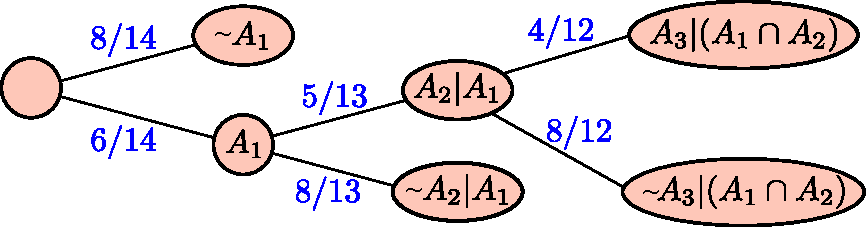
\includegraphics[width=\linewidth]{images/pcondicional1}
\end{image}%
\tcblower
\end{figureptx}%
A probabilidade de que a primeira bola seja branca é \(\frac{6}{14}\). Dado que aconteceu \(A_1\), a probabilidade de que a segunda bola seja branca é \(\frac{5}{13}\). Dado que aconteceram \(A_1\) e \(A_2\), a probabilidade de que a terceira bola seja branca é \(\frac{4}{12}\). Portanto%
\begin{equation*}
P(A_1\cap A_2\cap A_3) = \frac{6}{14}\cdot\frac{5}{13}\cdot\frac{4}{12} = \frac{5}{91} \approx 0.0549 \approx 5,5\% 
\end{equation*}
Na solução deste problema, usamos a Proposição 1 (Regra do Produto de Probabilidades)%
\end{fact}
\begin{proposition}{}{}{g:proposition:idp293}%
\terminology{(Regra do Produto de Probabilidades)}%
\par
Sejam \(A_1, A_2, \cdots, A_n\) eventos de um espaço amostral \(\Omega\) e \(P\) uma probabilidade em \(\Omega\). Se%
\begin{equation*}
P(A_1\cap A_2\cap \cdots \cap A_n) \neq 0, 
\end{equation*}
então%
\begin{align*}
P(A_1\cap A_2\cap \cdots \cap A_n) = \amp ~ P(A_1)\cdot P(A_2|A_1)\cdot P(A_3|(A_1\cap A_2))\cdots \\
\amp ~~~~ \cdots P(A_n|(A_1\cap A_2\cap \cdots \cap A_{n-1})). 
\end{align*}
%
\end{proposition}
\begin{proof}{}{g:proof:idp294}
Para dois conjuntos a fórmula é verdadeira, pois coincide com a definição de probabilidade condicional. Vamos usar o Princípio de Indução Completa para mostrar que o resultado é verdadeiro. Suponha o resultado válido para \(n-1\) eventos. Então%
\begin{align*}
\overbrace{P(A_1\cap A_2\cap \cdots \cap A_{n-1})}^{(\blacklozenge)} = \amp ~  P(A_1)\cdot P(A_2|A_1)\cdot P(A_3|(A_1\cap A_2))\cdots \\
\amp ~~~~ ~ \cdots P(A_{n-1}|(A_1\cap A_2\cap \cdots \cap A_{n-2})). 
\end{align*}
Defina \(B = A_1\cap A_2\cap \cdots \cap A_{n-1}\). Queremos a probabilidade \(P(B\cap A_n)\) e vamos usar que o resultado é válido para \(B\cap A_n\) e para \(n-1\) eventos. Logo%
\begin{align*}
P(B\cap A_n) = \amp ~  P(B)\cdot P(A_n|B) \\
= \amp  ~ \underbrace{P(A_1\cap A_2\cap \cdots \cap A_{n-1})}_{(\blacklozenge)}\cdot P(A_n|B). 
\end{align*}
Substituindo \((\blacklozenge)\) e \(B\) chegamos no resultado:%
\begin{align*}
P(A_1\cap A_2\cap \cdots \cap A_n) = \amp ~ P(A_1)\cdot P(A_2|A_1)\cdot P(A_3|(A_1\cap A_2))\cdots \\
\amp ~~~~ \cdots P(A_n|(A_1\cap A_2\cap \cdots \cap A_{n-1})). \qedhere
\end{align*}
%
\end{proof}
\begin{fact}{}{}{g:fact:idp295}%
Sabe-se que \(80\%\) das importações, por pessoas físicas, para o Brasil vem da China. A probabilidade de uma importação chegar na residência do comprador é de \(30\%\) se for uma compra da China e \(90\%\) caso contrário.  Se uma importação for feita agora.%
\par
a) Qual a probabilidade de que a compra ser da China e de chegar na residência do comprador?%
\par
b) Qual a probabilidade de que a compra chegue na residência do comprador?%
\par
c) Uma importação foi feita e o produto se perdeu. Qual a probabilidade de ter sido da china?%
\textbf{\blocktitlefont Solução 1}.\quad{}\terminology{item a)}%
\par
Usaremos as notações:%
\begin{align*}
C: \amp ~ \text{ é uma importação da China;} \\
R: \amp ~ \text{ o comprador Recebe a importação;} 
\end{align*}
Logo,%
\begin{align*}
P(C\cap R) = \amp ~ P(C) P(R|C) \\
= \amp ~ 0,8\times 0,3 = 0,24\\
= \amp 24\% 
\end{align*}
%
\par
\terminology{item b)}%
\par
Para uma importação chegar na residência do comprador, ela pode ter sido feita da china ou do complementar da china. Usaremos \(nR\) para dizer que não chegou na residência e \(nC\) para dizer que não é da china. A probabilidade de que a importação chegue é dada por%
\begin{equation*}
P(R) = \underbrace{P( (C\cap R) \cup (nC\cap R))}_{(\bigstar)} = P(C\cap R) + P(nC\cap R). 
\end{equation*}
Usando a \hyperref[x:remark:def-prob-condicional-p2]{Observação~{\xreffont\ref{x:remark:def-prob-condicional-p2}}}, temos%
\begin{align*}
P(R) = \amp ~ \overbrace{P(C)P(R|C) +P(nC)P(R|nC)}^{(\bigstar)} \\
= \amp ~ 0,8\times 0,3 + 0,2\times 0.9 = 42\%
\end{align*}
Nesta solução, usamos o \hyperref[x:theorem:teo-probabilidade-total]{Teorema~{\xreffont\ref{x:theorem:teo-probabilidade-total}}} (Teorema da Probabilidade Total).%
\par
\terminology{item c)}%
\par
Vamos calcular a probabilidade de que a importação seja da China e tenha se perdido, vamos dividir esse valor pela probabilidade de que a importação tenha se perdido.%
\par
A probabilidade de que a importação se perdeu e foi da china é de%
\begin{equation*}
P(C\cap nR) = 0,8\times 0,7 = 0,56 = 56\%. 
\end{equation*}
A probabilidade de que a importação tenha se perdido é dada por%
\begin{equation*}
P(nR) = 0,2\times 0,1 + 0,8\times 0,7 = 58\%.
\end{equation*}
Portanto a probabilidade de que tenha sido da china a  importação que se perdeu  é%
\begin{equation*}
\frac{P(C\cap nR)}{P(nR)} = \frac{0,56}{0,58} = 0.965517241379310 \approx 0,97\%.
\end{equation*}
Observe que o cálculo usado foi o seguinte:%
\begin{align*}
P(C|nR) = \amp ~\frac{P(C\cap nR)}{P(nR)} \\
= \amp ~ \frac{P(C)P(nR|C)}{P(nC\cap nR)+P(C\cap nR)}\\
= \amp ~ \frac{P(C)P(nR|C)}{P(nC)P(nR|nC)+P(C)P(nR|C)}
\end{align*}
Este é o \hyperref[x:theorem:teo-bayes]{Teorema~{\xreffont\ref{x:theorem:teo-bayes}}} Teorema de Bayes.%
\par\smallskip%
\noindent\textbf{\blocktitlefont Solução 2}.\quad{}\terminology{item b)}%
\par
Para organizar melhor as ideias, desenhamos uma árvore com todas as possibilidades.%
\begin{figureptx}{Árvore de Probabilidades.}{x:figure:fig-probabilidade-2}{}%
\begin{image}{0.2}{0.6}{0.2}%
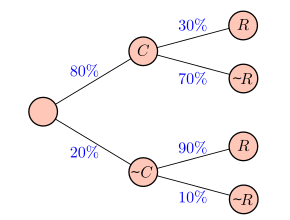
\includegraphics[width=\linewidth]{images/pcondicionalb}
\end{image}%
\tcblower
\end{figureptx}%
Observa-se mais facilmente que a probabilidade da importação chegar na residência é dada por%
\begin{equation*}
0,2\times 0,9 + 0,8\times 0,3 = 0,42=42\% 
\end{equation*}
%
\par
\terminology{item c)}%
\par
Usando a árvore de probabilidades, vamos calcular a probabilidade de que a importação seja da China e tenha se perdido, vamos dividir esse valor pela probabilidade de que a importação tenha se perdido.%
\begin{equation*}
\frac{0,8\times 0,7}{0,2\times 0,1 + 0,8\times 0,7} = \frac{0,56}{0,58} = 0,9655 \approx 97\%.
\end{equation*}
%
\end{fact}
\begin{theorem}{}{}{x:theorem:teo-probabilidade-total}%
\terminology{(Teorema da Probabilidade Total)}Sejam \(A_1, A_2, \ldots, A_n\) e \(B\) é um eventos tais que%
\begin{equation*}
B\subset A_1\cup A_2\cup\cdots \cup A_n, ~~~~ A_i\cap A_j = \emptyset, ~~\text{ para } i\neq j. 
\end{equation*}
e%
\begin{equation*}
P(A_i)>0,~~ i = 1, \ldots, n.  
\end{equation*}
então%
\begin{equation*}
P(B) = P(A_1)P(B|A_1) + P(A_2)P(B|A_2)+\cdots + P(A_n)P(B|A_n). 
\end{equation*}
%
\end{theorem}
\begin{proof}{}{g:proof:idp296}
Como vale%
\begin{equation*}
B\subset A_1\cup A_2\cup\cdots \cup A_n, ~~~~ A_i\cap A_j = \emptyset, ~~\text{ para } i\neq j. 
\end{equation*}
Temos%
\begin{equation*}
B = (A_1\cap B) \cup (A_2\cap B) \cup \cdots \cup (A_n\cap B). 
\end{equation*}
com a união disjunta, portanto%
\begin{align*}
P(B) = \amp ~ P(A_1\cap B) + P(A_2\cap B) + \cdots + P(A_n\cap B) \\
= \amp ~ P(A_1)P(B|A_1)+ P(A_2)P(B|A_2)+\cdots + P(A_n)P(B|A_n).\qedhere
\end{align*}
%
\end{proof}
\begin{theorem}{}{}{x:theorem:teo-bayes}%
\terminology{(Teorema de Bayes)}Sejam \(A_1, A_2, \ldots, A_n\) e \(B\) é um eventos tais que%
\begin{equation*}
B\subset A_1\cup A_2\cup\cdots \cup A_n, ~~~~ A_i\cap A_j = \emptyset, ~~\text{ para } i\neq j. 
\end{equation*}
e%
\begin{equation*}
P(A_i)>0,~~ i = 1, \ldots, n.  
\end{equation*}
então%
\begin{equation*}
P(A_i|B) = \frac{P(A_i)P(B|A_i)}{P(A_1)P(B|A_1)+\cdots +P(A_n)P(B|A_n)}. 
\end{equation*}
%
\end{theorem}
\begin{proof}{}{g:proof:idp297}
Aplicando a definição de probabilidade condicional, temos%
\begin{align*}
P(A_i|B) = \amp ~ \frac{P(B\cap A_i)}{P(B)} \\
= \amp ~ \frac{P(A_i)P(B|A_i)}{P(B)}.
\end{align*}
Usando o Teorema 2 e substituindo em \(P(B)\), obtemos%
\begin{equation*}
P(A_i|B) = \frac{P(A_i)P(B|A_i)}{P(A_1)P(B|A_1)+ P(A_2)P(B|A_2)+\cdots + P(A_n)P(B|A_n)}.\qedhere
\end{equation*}
%
\end{proof}
%
%
\typeout{************************************************}
\typeout{Exercícios 5.2.1 Exercícios}
\typeout{************************************************}
%
\begin{exercises-subsection}{Exercícios}{}{Exercícios}{}{}{g:exercises:idp298}
\begin{divisionexercise}{1}{}{}{g:exercise:idp299}%
Dois dados \(D_1\) e \(D_2\) são lançados e os resultados nas faces de cima anotados.%
\begin{enumerate}[label=(\alph*)]
\item{}Qual a probabilidade da soma dos pontos ser 6, se a face observada em \(D_1\) foi 2?%
\item{}Qual a probabilidade de ter saı́do 2 em \(D_1\) , se a soma dos pontos foi 6?%
\item{}Qual a probablidade da soma dos pontos ser menor do que 7, sabendo que o número 2 saiu pelo menos uma vez?%
\item{}Qual a probabilidade da soma dos pontos ser menor do que ou igual a 6, se o maior dos números obtidos é menor do que 5?%
\item{}Qual a probabilidade do maior dos números obtidos ser menor do que 5, sabendo que a soma dos pontos foi menor do que ou igual a 6?%
\end{enumerate}
%
\par\smallskip%
\noindent\textbf{\blocktitlefont Resposta}.\hypertarget{g:answer:idp300}{}\quad{}a) \(\dfrac{1}{6}\), b) \(\dfrac{1}{5}\), c) \(\dfrac{7}{11}\), d) \(\dfrac{13}{16}\), e) \(\dfrac{13}{15}\).%
\end{divisionexercise}%
\begin{divisionexercise}{2}{}{}{g:exercise:idp301}%
Três caixas I, II e III contém respectivamente 1 bola branca e 2 pretas; 2 brancas e 1 preta; 3 brancas e 2 pretas. Uma caixa é escolhida ao acaso e dela é retirada uma bola. Determine a probabilidade:%
%
\begin{enumerate}[label=(\alph*)]
\item{}da bola retirada ser branca, sabendo que a caixa escolhida foi a I;%
\item{}da caixa escolhida ter sido a I e a bola retirada ser branca.%
\end{enumerate}
\par\smallskip%
\noindent\textbf{\blocktitlefont Resposta}.\hypertarget{g:answer:idp302}{}\quad{}a) \(\dfrac{1}{3}\), b) \(\dfrac{1}{9}\).%
\end{divisionexercise}%
\begin{divisionexercise}{3}{}{}{g:exercise:idp303}%
Uma caixa contém 30 bolas pretas, 20 brancas e 10 vermelhas. Três bolas são retiradas da caixa, uma após a outra, sem reposição. Qual a pobabilidade da terceira bola retirada ser preta?%
\par\smallskip%
\noindent\textbf{\blocktitlefont Resposta}.\hypertarget{g:answer:idp304}{}\quad{}\(\dfrac{1}{2}\)%
\end{divisionexercise}%
\end{exercises-subsection}
\end{sectionptx}
%
%
\typeout{************************************************}
\typeout{Seção 5.3 Distribuição Binomial}
\typeout{************************************************}
%
\begin{sectionptx}{Distribuição Binomial}{}{Distribuição Binomial}{}{}{x:section:section-distribuicao-binomial}
\begin{objectives}{Objetivos}{x:objectives:objetivos-distribuicao-binomial}
%
\begin{enumerate}
\item{}Definir Eventos Independentes.%
\item{}Enunciar e demonstrar o Teorema da Distribuição Binomial.%
\item{}Exemplificar.%
\end{enumerate}
\end{objectives}
%
%
\typeout{************************************************}
\typeout{Subseção 5.3.1 Eventos Independentes}
\typeout{************************************************}
%
\begin{subsectionptx}{Eventos Independentes}{}{Eventos Independentes}{}{}{g:subsection:idp305}
\begin{definition}{}{g:definition:idp306}%
Sejam \(A\) e \(B\) eventos.  \(A\) e \(B\) são \emph{independentes} se,%
\begin{equation*}
P(B|A) = P(B). 
\end{equation*}
%
\par
Da \hyperref[x:remark:def-prob-condicional-p2]{Observação~{\xreffont\ref{x:remark:def-prob-condicional-p2}}}, temos%
%
\begin{equation*}
P(A\cap B) = P(A)\cdot P(B|A) = P(A)\cdot P(B). 
\end{equation*}
\end{definition}
\begin{fact}{}{}{g:fact:idp307}%
Em um experimento aleatório é retirado sucessivamente, com reposição, duas bolas de uma caixa que comtém 8 bolas pretas e 6 bolas brancas. Qual a probabilidade de que sejam duas bolas brancas?%
\textbf{\blocktitlefont Solução}.\quad{}Considere os eventos:%
\begin{equation*}
A_1: \text{ a primeira bola é branca;}\\
A_2: \text{ a segunda bola é branca;}\\
\end{equation*}
Observe que os eventos são independentes, portanto a probabilidade é%
\begin{align*}
P(A_1\cap A_2) = \amp ~ P(A_1)\cdot P(A_2)\\
= \amp ~ \frac{6}{14}\cdot \frac{6}{14} \\
= \amp ~\frac{9}{49} \\
= \amp ~ 0.18367 \\
\approx \amp ~ 18,37\%. 
\end{align*}
%
\end{fact}
\begin{definition}{}{g:definition:idp308}%
Sejam \(A_1, A_2, \ldots, A_n\) eventos.  \(A_1, A_2, \ldots, A_n\) são \emph{independentes} se, para todo \(k\), \(1 \leq k \leq n\) e para quaisquer \(i_1, i_2, \ldots, i_k\in \{1, 2, \ldots, n\}\), tem-se%
\begin{equation*}
P(A_k|A_{i_1}\cap A_{i_2}\cap \cdots \cap A_{i_k}) = P(A_k). 
\end{equation*}
Consequentemente,%
%
\begin{equation*}
P(A_{1}\cap A_{2}\cap \cdots \cap A_{n}) = P(A_{1})\cdot P(A_{2})\cdots P(A_{n}). 
\end{equation*}
%
\end{definition}
\begin{fact}{}{}{g:fact:idp309}%
Em um experimento aleatório é retirado sucessivamente, com reposição, três bolas de uma caixa que comtém 8 bolas pretas e 6 bolas brancas. Qual a probabilidade de que sejam três bolas brancas?%
\textbf{\blocktitlefont Solução}.\quad{}Considere os eventos:%
\begin{equation*}
A_1: \text{ a primeira bola é branca;}\\
A_2: \text{ a segunda bola é branca;}\\
A_3: \text{ a terceira bola é branca;}\\
\end{equation*}
Observe que os eventos são independentes, portanto a probabilidade é%
\begin{align*}
P(A_1\cap A_2\cap A_3) = \amp ~ P(A_1)\cdot P(A_2)\cdot P(A_3) \\
= \amp ~ \frac{6}{14}\cdot \frac{6}{14}\cdot \frac{6}{14} \\
= \amp ~\frac{27}{343} \\
= \amp ~ 0.07871 \\
\approx \amp ~ 7,9\%. 
\end{align*}
%
\end{fact}
\begin{fact}{}{}{g:fact:idp310}%
Um dado (não viciado) é lançado 5 vezes. Qual é a probabilidade de obtermos os resultados \(1, 2, 3, 2, 1\), exatamente nessa ordem?%
\textbf{\blocktitlefont Solução}.\quad{}Seja \(A_i\) o evento: saiu o valor da posição \(i\) da lista \([1, 2, 3, 2, 1]\), no \(i\)-ésimo lançamento, \(i\in\{1, 2, 3, 4, 5\}\).%
\par
Como os eventos são independentes, temos%
\begin{align*}
P(A_1\cap A_2\cap \cdots \cap A_{5}) = \amp ~ P(A_1)\cdot P(A_2)\cdots P(A_{5}) \\
= \amp ~ \left(\frac{1}{6}\right)^{5} \\
= \amp ~\frac{1}{7776} \\
= \amp ~ 0.0001286 \\
\approx \amp ~ 0,013\%. 
\end{align*}
%
\end{fact}
\end{subsectionptx}
%
%
\typeout{************************************************}
\typeout{Subseção 5.3.2 Distribuição Binomial}
\typeout{************************************************}
%
\begin{subsectionptx}{Distribuição Binomial}{}{Distribuição Binomial}{}{}{g:subsection:idp311}
\begin{fact}{}{}{g:fact:idp312}%
Jogando uma moeda não viciada 15 vezes. Qual é a probabilidade de obtermos exatamente 7 caras?%
\textbf{\blocktitlefont Solução}.\quad{}Os eventos são independentes e a probabilidade de obter cara no lançamento da moeda é \(p=\frac{1}{2}\).%
\par
Queremos achar a probabilidade de obtermos 7 caras em 15 lançamentos. Vamos, inicialmente, fixar que queremos os 7 primeiros resultados iguais a cara, assim estamos impondo que os 8 resultados seguintes serão coroa. Desta forma, a probabilidade de que os 7 primeiros resultados sejam cara e de que os 8 resultados seguintes sejam coroa é %
\begin{equation*}
\left(\frac{1}{2}\right)^7 \times \left(1 - \frac{1}{2}\right)^{8},
\end{equation*}
mas a pergunta do problema não foi esta, pois a ordem em que apareceram as caras e as coroas não importa.%
\par
Observe que o número de formas de ordenar 7 caras e 8 coroas coincide com o número formas de escolher 7 lugares, para colocar as caras, dentre 15 disponíveis, e colocar as coroas nos lugares que sobraram. Isto pode ser feito de \(C_{15}^{7}\) maneiras.%
\par
Portanto a resposta para nosso problema é%
\begin{equation*}
C_{15}^{7}\times \left(\frac{1}{2}\right)^7 \times \left(\frac{1}{2}\right)^{8}=0.1963 \approx 20\%. 
\end{equation*}
%
\end{fact}
\begin{theorem}{}{}{x:theorem:teo-dist-binomial}%
Considere um experimento com apenas dois resultados possíveis, chamados de \emph{sucesso} e \emph{fracasso}. Denotaremos por \(p\) a probabilidade de sucesso.%
\par
A probabilidade de ocorrerem exatamente \(k\) sucessos em uma sequência de \(n\) provas independentes, na qual a probabilidade de sucesso em cada etapa é \(p\), é igual a%
\begin{equation*}
C_n^k\times p^k\times (1-p)^{n-k}. 
\end{equation*}
%
\end{theorem}
\begin{proof}{}{g:proof:idp313}
A probabilidade de nessas \(n\) provas obtermos \(k\) sucessos, e consequentemente, \(n-k\) fracassos em uma ordem fixada é%
\begin{equation*}
\underbrace{p\cdot p \cdots p}_{k\text{ fatores}}\underbrace{\cdot (1-p)\cdots(1-p)}_{(n-k)\text{ fatores}} = p^k(1-p)^{n-k}, 
\end{equation*}
pois as provas são independentes. É claro que em outra ordem, a probabilidade seria a mesma, pois apenas a ordem dos fatores se altera. Como o número de formas de alterar esta ordem é \(C_n^k\), a probabilidade de obtermos \(k\) sucessos, em \(n\) provas é%
\begin{equation*}
C_n^k \times p^k\times(1-p)^{n-k}. \qedhere
\end{equation*}
%
\end{proof}
\begin{fact}{}{}{g:fact:idp314}%
Um dodecaedro (regular, com peso uniforme, ou seja, não viciado) tem 3 faces verdes e 4 faces vermelhas e 5 faces azuis.%
\par
a) Qual é a probabilidade de em 8 lançamentos desse dodecaedro, obtermos 3 vezes a cor verde?%
\par
b) Qual é a probabilidade de em 8 lançamentos desse dodecaedro, obtermos 3 vezes a cor azul?%
\textbf{\blocktitlefont Solução}.\quad{}\terminology{item a)} Vamos considerar os eventos:%
\par
S: saiu uma face verde \(\Rightarrow p = \frac{3}{12} = \frac{1}{4}.\)%
\par
F: não saiu uma face verde \(\Rightarrow p = \frac{9}{12} = \frac{3}{4}.\)%
\par
Pelo \hyperref[x:theorem:teo-dist-binomial]{Teorema~{\xreffont\ref{x:theorem:teo-dist-binomial}}} a probabilidade é%
\begin{equation*}
C_8^3\times \left( \frac{1}{4} \right)^3 \times \left( \frac{3}{4} \right)^5 = \frac{1701}{8192} \approx 0.20764 \approx 21\%. 
\end{equation*}
%
\par
\terminology{item b)} Vamos considerar os eventos:%
\par
S: saiu uma face azul \(\Rightarrow p = \frac{5}{12}.\)%
\par
F: não saiu uma face azul \(\Rightarrow p = \frac{7}{12}.\)%
\par
Pelo \hyperref[x:theorem:teo-dist-binomial]{Teorema~{\xreffont\ref{x:theorem:teo-dist-binomial}}} a probabilidade é%
%
\begin{equation*}
C_8^3\times \left( \frac{5}{12} \right)^3 \times \left( \frac{7}{12} \right)^5 = \frac{14706125}{53747712} \approx 0.27361 \approx 27,4\%. 
\end{equation*}
\end{fact}
\end{subsectionptx}
%
%
\typeout{************************************************}
\typeout{Exercícios 5.3.3 Exercícios}
\typeout{************************************************}
%
\begin{exercises-subsection}{Exercícios}{}{Exercícios}{}{}{g:exercises:idp315}
\begin{divisionexercise}{1}{}{}{g:exercise:idp316}%
Em um torneio de ping-pong, um jogador \(J_1\) deve enfrentar outros dois jogadores \(J_2\) e \(J_3\). Os resultados dos jogos são independentes e as probabilidades de \(J_1\) ganhar de \(J_2\) e de \(J_3\) são \(1/3\) e \(2/3\) respectivamente. O jogador vencerá o terneiro se ganhar dois jogos consecutivos, de uma série de 3.%
\par
Que série é mais favorável para o jogador:%
\begin{equation*}
J_2J_3J_2 ~~\text{ ou }~~ J_3J_2J_3?
\end{equation*}
%
\par\smallskip%
\noindent\textbf{\blocktitlefont Resposta}.\hypertarget{g:answer:idp317}{}\quad{}\(J_2J_3J_2\)%
\end{divisionexercise}%
\begin{divisionexercise}{2}{}{}{g:exercise:idp318}%
Uma caixa contém 9 bolas brancas, 6 pretas e 5 vermelhas. Retiram-se, sucessivamente e com reposição, 4 bolas dessa caixa. Determine a probabilidade:%
\begin{enumerate}[label=(\alph*)]
\item{}das 4 bolas retiradas serem vermelhas;%
\item{}de somente 2 bolas retiradas serem vermelhas;%
\item{}de pelo menos 2 bolas serem vermelhas.%
\end{enumerate}
%
\par\smallskip%
\noindent\textbf{\blocktitlefont Resposta}.\hypertarget{g:answer:idp319}{}\quad{}a) \(\dfrac{1}{256}\), b) \(\dfrac{27}{128}\), c) \(\dfrac{67}{256}\).%
\end{divisionexercise}%
\end{exercises-subsection}
\end{sectionptx}
\end{chapterptx}
%
%
\typeout{************************************************}
\typeout{Referêcias 6 Referências Bibliográficas}
\typeout{************************************************}
%
\begin{references-}{Referências Bibliográficas}{}{Referências Bibliográficas}{}{}{x:references:referencias}
\terminology{Livros}%
%% If this is a top-level references
%%   you can replace with "thebibliography" environment
\begin{referencelist}
\bibitem[1]{x:biblio:morgado}\hypertarget{x:biblio:morgado}{}  Morgado, A. C. O., et al, \href{https://loja.sbm.org.br/index.php/analise-combinatoria-e-probabilidade.html}{Análise Combinatória e Probabilidade}, SBM. 6ª ed.
\bibitem[2]{g:biblio:idp320}\hypertarget{g:biblio:idp320}{}  Niven, I., \textit{Mathematics of Choice: How to Count Without Counting}, The Mathematical Associations of America.
\bibitem[3]{g:biblio:idp321}\hypertarget{g:biblio:idp321}{}  Rosen, K. H., \textit{Discrete Mathematics and Its Applications}, McGraw-Hill.
\bibitem[4]{g:biblio:idp322}\hypertarget{g:biblio:idp322}{}  Silva, L. D. ; Santos, M. P. ; Machado J. R. N., \href{https://loja.sbm.org.br/index.php/elementos-de-computac-o-matematica-com-sagemath.html}{Elementos de Computação Matemática com SageMath}, SBM, 1ª ed.
\bibitem[5]{g:biblio:idp323}\hypertarget{g:biblio:idp323}{}  Bezerra, N., \href{https://livroaberto.ufpa.br/jspui/bitstream/prefix/480/1/Livro_AnaliseCombinatoriaProbabilidade.pdf}{Análise Combinatória e Probabilidade}, editAedi.
\bibitem[6]{g:biblio:idp324}\hypertarget{g:biblio:idp324}{}  Morgado, A. C. ; Carvalho, P. C. P., \href{https://loja.sbm.org.br/index.php/colecoes/sbm/colecao-profmat/matematica-discreta.html}{Matemática Discreta}, SBM: coleção PROFMAT, 2ª ed.
\bibitem[7]{g:biblio:idp325}\hypertarget{g:biblio:idp325}{}  Lovász, L. ; Pelikán, J. ; Vesztergombi, K., \textit{Discrete Mathematics: Elementary and Beyond}, Springer.
\terminology{Artigos}%
\bibitem[8]{x:biblio:oxente01}\hypertarget{x:biblio:oxente01}{}  Machado J. R. N., \href{http://ematematicaoxente.com.br/wp-content/uploads/2018/12/jornal_9ed.pdf}{O Princípio da Casa dos Pombos}, Jornal de Matemática Olímpica UFRPE, 2018.
\terminology{Dissertações}%
\bibitem[9]{x:biblio:luiz}\hypertarget{x:biblio:luiz}{}  Santana Neto, L. M., \textit{Análise Combinatória: Lemas de Kaplansky, Permutações Caóticas, O Princípio da Casa Dos Pombos e suas Aplicações na Matemática do Ensino Médio}, Dissertação do ProfMat.
\end{referencelist}
\end{references-}
\end{document}